\documentclass{jknotes}
\usepackage{../joshkirklin}

\setmathfont{Latin Modern Math}
\setmathfont{GFS NeoHellenic Math}[range=bfsfup/{greek,Greek}->it]
\setmathfont{GFS NeoHellenic Math}[range=sfup/{latin,Latin}->it]

\usetikzlibrary{shapes.misc}

\tikzset{cross/.style={cross out, draw=black, minimum
size=2*(#1-\pgflinewidth), inner sep=0pt, outer sep=0pt}}
%default radius will be 1pt. 

\begin{document}

\institution{Cambridge Part III Maths}
\title{Fluid Dynamics of Climate}
\lecturer{John Taylor \& Peter Haynes}
\notetaker{Charles Powell}
\date{Michaelmas 2020}

\maketitle
\suggestionsspiel
\tableofcontents

\lecture{12/10/20}
\section{Introduction}
\subsection{Fluid motion in a rotating reference frame}
In a non-rotating frame, the \emph{Navier-Stokes} equations are
\begin{equation}
	\rho \frac{\diffD \symbf{u}}{\diffD t} = -\nabla p - \rho \nabla \phi + \rho
	\symbf{F}
	\label{ns}
\end{equation}

The body forces are assumed to be conservative with potential $\phi$, e.g.
$\phi = gz$ for gravitational force. $\symbf{F}$ is the frictional force.

Consider a reference frame rotating about the $z$-axis with constant angular
velocity $\symbf{\Omega}$. Axes in the inertial frame are denoted with a
subscript $_I$ and axes in the rotating frame are denoted with a subscript
$_R$.

\begin{center}
\newcommand{\TikzInnerSep}{0.33mm}

% Define new arc command
% Syntax: [draw options] (center) (initial angle:final angle:radius)
% https://tex.stackexchange.com/a/66220
\def\centerarc[#1](#2)(#3:#4:#5){%
	\draw [#1] ($(#2)+({#5*cos(#3)}, {#5*sin(#3)})$) arc (#3:#4:#5)%
}

% Redefine the rotation sequence for the tikz3d-plot to Euler-Angles:
% z-x-z with alpha-beta-gamma (psi-theta-phi)
% https://tex.stackexchange.com/q/118069/98906
\newcommand{\tdseteulerzxz}{%
	\renewcommand{\tdplotcalctransformrotmain}{%
		%
		% Determine the sin and cos of the specified angle in degrees
		% \tdplotsinandcos{sin}{cos}{theta}
		% - #1: Returns sin(#3)
		% - #2: Returns cos(#3)
		% - #3: User-specified angle theta
		\tdplotsinandcos{\sinalpha}{\cosalpha}{\tdplotalpha} 
		\tdplotsinandcos{\sinbeta}{\cosbeta}{\tdplotbeta}
		\tdplotsinandcos{\singamma}{\cosgamma}{\tdplotgamma}
		%
		% Define trigonometric abbreviations
		%
		\tdplotmult{\sasb}{\sinalpha}{\sinbeta}
		\tdplotmult{\sacb}{\sinalpha}{\cosbeta}
		\tdplotmult{\sacbsg}{\sacb}{\singamma}
		\tdplotmult{\sacbcg}{\sacb}{\cosgamma}
		\tdplotmult{\sasg}{\sinalpha}{\singamma}
		\tdplotmult{\sacg}{\sinalpha}{\cosgamma}
		%
		\tdplotmult{\sbsg}{\sinbeta}{\singamma}
		\tdplotmult{\sbcg}{\sinbeta}{\cosgamma}
		%
		\tdplotmult{\casb}{\cosalpha}{\sinbeta}
		\tdplotmult{\cacb}{\cosalpha}{\cosbeta}
		\tdplotmult{\cacbsg}{\cacb}{\singamma}
		\tdplotmult{\cacbcg}{\cacb}{\cosgamma}
		\tdplotmult{\casg}{\cosalpha}{\singamma}
		\tdplotmult{\cacg}{\cosalpha}{\cosgamma}
		%
		% Define the entries for the rotation matrix from the B-System to the I-System
		% This is A_IB = (A_BI)^T
		%
		\pgfmathsetmacro{\raaeul}{+\cacg - \sacbsg}
		\pgfmathsetmacro{\rabeul}{-\casg - \sacbcg}
		\pgfmathsetmacro{\raceul}{+\sasb}
		%
		\pgfmathsetmacro{\rbaeul}{+\sacg + \cacbsg}
		\pgfmathsetmacro{\rbbeul}{-\sasg + \cacbcg}
		\pgfmathsetmacro{\rbceul}{-\casb}
		%
		\pgfmathsetmacro{\rcaeul}{+\sbsg}
		\pgfmathsetmacro{\rcbeul}{+\sbcg}
		\pgfmathsetmacro{\rcceul}{+\cosbeta}
		%
	}
}

% Redefine the rotation sequence for the tikz3d-plot to Cardan-Angles:
% x-y-z with alpha-beta-gamma
% https://tex.stackexchange.com/q/118069/98906
\newcommand{\tdsetcardanxyz}{%
	\renewcommand{\tdplotcalctransformrotmain}{%
		%
		% Determine the sin and cos of the specified angle in degrees
		% \tdplotsinandcos{sin}{cos}{theta}
		% - #1: Returns sin(#3)
		% - #2: Returns cos(#3)
		% - #3: User-specified angle theta
		\tdplotsinandcos{\sinalpha}{\cosalpha}{\tdplotalpha} 
		\tdplotsinandcos{\sinbeta}{\cosbeta}{\tdplotbeta}
		\tdplotsinandcos{\singamma}{\cosgamma}{\tdplotgamma}
		%
		% Define trigonometric abbreviations
		%
		\tdplotmult{\sasb}{\sinalpha}{\sinbeta}
		\tdplotmult{\sasbsg}{\sasb}{\singamma}
		\tdplotmult{\sasbcg}{\sasb}{\cosgamma}
		%
		\tdplotmult{\sacb}{\sinalpha}{\cosbeta}
		\tdplotmult{\sasg}{\sinalpha}{\singamma}
		\tdplotmult{\sacg}{\sinalpha}{\cosgamma}
		%
		\tdplotmult{\casb}{\cosalpha}{\sinbeta}
		\tdplotmult{\casbsg}{\casb}{\singamma}
		\tdplotmult{\casbcg}{\casb}{\cosgamma}
		%
		\tdplotmult{\cacb}{\cosalpha}{\cosbeta}
		\tdplotmult{\casg}{\cosalpha}{\singamma}
		\tdplotmult{\cacg}{\cosalpha}{\cosgamma}
		\tdplotmult{\cbsg}{\cosbeta}{\singamma}
		\tdplotmult{\cbcg}{\cosbeta}{\cosgamma}
		%
		% Define the entries for the rotation matrix from the B-System to the I-System
		% This is A_IB = (A_BI)^T
		%
		\pgfmathsetmacro{\raaeul}{+\cbcg}
		\pgfmathsetmacro{\rabeul}{-\cbsg}
		\pgfmathsetmacro{\raceul}{+\sinbeta}
		%
		\pgfmathsetmacro{\rbaeul}{+\casg + \sasbcg}
		\pgfmathsetmacro{\rbbeul}{+\cacg - \sasbsg}
		\pgfmathsetmacro{\rbceul}{-\sacb}
		%
		\pgfmathsetmacro{\rcaeul}{+\sasg - \casbcg}
		\pgfmathsetmacro{\rcbeul}{+\sacg + \casbsg}
		\pgfmathsetmacro{\rcceul}{+\cacb}
		%
	}
}

% Plot display orientation
\tdplotsetmaincoords{70}{150}

% Rotation angles Euler
\pgfmathsetmacro{\zOneRot}{25}
\pgfmathsetmacro{\xRot}{15}
\pgfmathsetmacro{\zTwoRot}{30}

\begin{tikzpicture}[x = 1.0cm, y = 1.0cm, z = 1.0cm, scale = 2.5, tdplot_main_coords]
	\coordinate (Origin) at (0, 0, 0);
	
	% x_I
	\draw [arrows = {}-{latex}, line width = 1.0pt] (Origin) -- (1, 0, 0)%
		node[anchor = east, xshift = -1mm, inner sep = \TikzInnerSep]%
			{$\VL{x}_I$};
	% Set the FoR orientation
	\tdseteulerzxz
	\tdplotsetrotatedcoords{\zOneRot}{0}{0}
	% x_1
	\draw [tdplot_rotated_coords, arrows = {}-{latex}, line width = 1.0pt,red] (Origin) -- (1, 0, 0)%
		node[anchor = north, yshift = -1mm, inner sep = \TikzInnerSep]%
			{$\VL{x}_R$};
	%
	% y_1
	\draw [tdplot_rotated_coords, arrows = {}-{latex}, line width = 1.0pt,red] (Origin) -- (0, 1, 0)%
		node[anchor = west, xshift = +1mm, yshift = +1mm, inner sep = \TikzInnerSep]%
			{$\VL{y}_R$};
	%
	% Draw selected axes over the grid
	% y_I
	\draw [arrows = {}-{latex}, line width = 1.0pt] (Origin) -- (0, 1, 0)%
		node[anchor = north west, xshift = +1mm, inner sep = \TikzInnerSep]%
			{$\VL{y}_I$};
	%
	% z_1
	\draw [tdplot_rotated_coords, arrows = {}-{latex},red, line width = 1.0pt] (Origin) -- (0, 0, 1)%
		node[anchor = south west, xshift = +1mm, yshift = -1mm, inner sep = \TikzInnerSep]%
		{$\textcolor{black}{\VL{z}_I} \; \textcolor{black}{=} \; \textcolor{red}{\VL{z}_R}$};
	
	% Draw rotation arrow
	\centerarc[tdplot_rotated_coords, canvas is yx plane at z=0.7, arrows = {latex}-{}](0, 0)(230 : 570 : 0.15)%
		node[anchor = north west, xshift = +2mm, yshift = -3mm, inner sep = \TikzInnerSep]%
		{$\left|\symbf{\Omega}\right| = \frac{\mathrm{d}\theta}{\mathrm{d}t}$};

	\centerarc[tdplot_rotated_coords, canvas is yx plane at z=0, arrows =
	{latex}-{}](0,0)(90:90+\zOneRot:0.6) node[midway,anchor= south] {$\theta$};

\end{tikzpicture}

\end{center}

For a point with position vector $\symbf{x}$ and velocity $\symbf{u}_R =
\left(\frac{\diffd \symbf{x}}{\diffd t}\right)_R$ in the rotating reference
frame
\begin{equation}
	\left(\frac{\diffd \symbf{x}}{\diffd t}\right)_I = 
	\left(\frac{\diffd \symbf{x}}{\diffd t}\right)_R + \symbf{\Omega} \times \symbf{x}
\end{equation}
or equivalently $\symbf{u}_I = \symbf{u}_R + \symbf{\Omega} \times \symbf{x}$. Hence the
acceleration is
\begin{equation}
	\begin{aligned}
		\left(\frac{\diffd \symbf{u}}{\diffd t}\right)_I &= 
	\left(\frac{\diffd}{\diffd t}\left[ \symbf{u}_R + \symbf{\Omega} \times \symbf{x}
			\right]\right)_R + \symbf{\Omega} \times \left( \symbf{u}_R +
		\symbf{\Omega} \times \symbf{x}\right)_R \\
		&= \left(\frac{\diffd \symbf{u}_R}{\diffd t}\right)_R + 2 \symbf{\Omega}
		\times \symbf{u}_R + \symbf{\Omega} \times \left( \symbf{\Omega} \times
		\symbf{x}\right)
	\end{aligned}
\end{equation}

The first term is the acceleration in the rotating frame, the second term is
the \emph{Coriolis acceleration} and the third term is the \emph{centrifugal
accelertion}. Note that we can write the centrifugal acceleration in the form
of a conservative force
\begin{equation}
	\begin{aligned}
		\symbf{\Omega} \times \left( \symbf{\Omega} \times \symbf{x}\right) &= \nabla
	\phi_c \\
	\phi_c &= -\frac{1}{2} \left| \symbf{\Omega} \times \symbf{x} \right|^2
\end{aligned}
\end{equation}

Hence the Navier-Stokes equations in a rotating reference frame are
\begin{equation}
	\rho \left( \frac{\diffD \symbf{u}}{\diffD t} + 2 \symbf{\Omega} \times
	\symbf{u}\right) = - \nabla p - \rho \nabla \left( \phi + \phi_c\right) +
	\rho \symbf{F} \label{nsrot}
\end{equation}

We group the potential terms into a \emph{geopotential} $\Phi \equiv \phi +
\phi_c$. The surface of a stationary ocean or atmosphere has a constant
\emph{geopotential height} described by an oblate spheroid.

\begin{figure}
\begin{center}
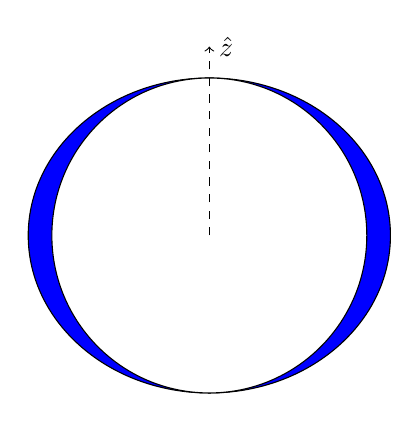
\begin{tikzpicture}
\filldraw [draw=black,fill=blue] (0,0) ellipse (2.3 and 2);
\filldraw [draw=black,fill=white] (0,0) circle (2);
\draw [dashed, ->] (0,0) -- (0,2.4) node[right] {$\hat{\symbf{z}}$};
\end{tikzpicture}
\caption{Geopotential ocean surface relative to a spherical Earth.}
\label{fig:oblate}
\end{center}
\end{figure}

Imagine a spherical earth. At sea level, the polar radius is 21.4km smaller
than the equatorial radius: see figure~\ref{fig:oblate}. In reality, the
surface of the Earth is also very close to a geopotential surface. Hence
\emph{geopotential coordinates} are very useful for planetary scale motion.

\subsubsection{Local Cartesian coordinates}
For small motions, it is much more convenient to define \emph{local Cartesian
coordinates} (figure~\ref{fig:lcc}).
\begin{figure}
	\begin{center}
	\begin{tikzpicture}
		\draw (0,0) circle (1.5);
		\draw (0,0) -- (1.5, 0) node[right] {Equator};
		\draw (0,0) -- (1.3, 0.75);
		\draw (0.6,0) arc (0:30:0.6) node[anchor = south] {$\theta$};
		\draw[->] (0,1.3) -- (0, 1.9);
		\draw[->] (0, 1.7) [partial ellipse = -180:70:0.3 and 0.1];
		\draw[->] (1.3, 0.75) -- (1.9,1.1) node[right] {\small $\hat{\symbf{z}}$};
		\draw[->] (1.3, 0.75) -- (1.3 - 0.35, 0.75 + 0.6) node[above] {\small
		$\hat{\symbf{y}}$};
		\draw (1.3, 0.75) circle (0.1) node[right] {\small $\hat{\symbf{x}}$};
	\end{tikzpicture}
	\caption{Local Cartesian coordinates}
	\label{fig:lcc}
	\end{center}
\end{figure}

In this coordinate system $\symbf{\Omega} = (0, \Omega \cos \theta, \Omega \sin
\theta)$. Hence if $\symbf{u} = (u, v, w)$ then
\begin{equation}
	\begin{aligned}
		2 \symbf{\Omega} \times \symbf{u} &= (2\Omega w \cos \theta - 2 \Omega v \sin
		\theta, 2 \Omega u \sin \theta, -2\Omega u \cos \theta) \\
		&= (-fv + f^* w, fu - f^* u)
	\end{aligned}
\end{equation}
where $f \equiv 2 \Omega \sin \theta$ is the \emph{Coriolis parameter} and
$f^* \equiv 2 \Omega \cos \theta$.

\begin{eg}
	In Cambridge, $\theta = 52.1^{\circ} N$ so
	\begin{equation}
		\begin{aligned}
			f &= 2 \Omega \sin \theta \\
			  &= 2 \cdot \frac{2\pi}{3600 \cdot 24} \cdot 0.79 s^{-1} \\
			  &\approx 1.14 \times 10^{-4} s^{-1}
		\end{aligned}
	\end{equation}
	At mid-latitudes, $f \sim 10^{-4}$ is a good approximation.
\end{eg}

We can simplify the Coriolis acceleration expression; often $f^* w \ll f v$
and $f^* u \ll g$. Hence
\begin{equation}
	2 \symbf{\Omega} \times \symbf{u} \approx (-fv, fu, 0) = f \hat{\symbf{z}} \times
	\symbf{u}
\end{equation}

This is the \emph{traditional approximation}. This is \emph{not} always a good
approximation, particularly at intermediate scales.

\subsubsection{Scale analysis.}
Define characteristic scales for length $L$, time $T$, and velocity $U$.
Non-dimensional variables are denoted with a superscript star: $\symbf{u}^* =
\symbf{u}/U$, etc.

Using these scalings with $\symbf{F} = \nu \nabla^2 \symbf{u}$ we have
\begin{equation}
	\frac{U}{T} \frac{\partial \symbf{u}^*}{\partial t^*} + \frac{U^2}{L}
	\symbf{u}^* \cdot \nabla^* \symbf{u}^* + fU \hat{\symbf{z}} \times \symbf{u}^* =
	-\frac{1}{\rho} \nabla \left(p + \rho \Phi\right) + \frac{\nu U}{L^2} \nabla_*^2
		\symbf{u}^*
\end{equation}

Dividing through by $fU$ leaves the Coriolis acceleration term $\text{ord}(1)$ with
other terms scaled relatively.
\begin{equation}
	\frac{1}{fT} \frac{\partial \symbf{u}^*}{\partial t^*} + \text{Ro}	\symbf{u}^*
	\cdot \nabla^* \symbf{u}^* + \hat{\symbf{z}} \times \symbf{u}^* =
	-\frac{1}{\rho f U} \nabla \left(p + \rho \Phi\right) + \text{E} \nabla_*^2
		\symbf{u}^*
\end{equation}
where $\text{Ro} \equiv \frac{U}{fL}$ is the \emph{Rossby number} and
$\text{E} \equiv \frac{\nu}{fL^2}$ is the \emph{Ekman number}.

\begin{eg}
	For an atmospheric storm, $U \sim 10 m s^{-1}, L \sim 1000 km, f \sim
	10^{-4} s^{-1}$. Thus $\text{Ro} \sim 0.1, \text{E} \sim 10^{-13}$.
\end{eg}

\lecture{14/10/2020}
Further, if $T = L/U$, then $\text{Ro} = U/fL = 1/fT$. For small \Ro, \Ek, 
on surfaces of constant $\Phi$, $f \hat{\symbf{z}} \times \symbf{u} \approx
-\frac{1}{\rho}\nabla p$.  This is \emph{geostrophic balance}. In components,
we have
\begin{equation}
	\begin{aligned}
		-fv &= -\frac{1}{\rho}\frac{\partial p}{\partial x} \\
		fu &= -\frac{1}{\rho}\frac{\partial p}{\partial y}
	\end{aligned}
\end{equation}
The equations of geostrophic balance can be arranged to give the horizontal
velocity:
$\symbf{u}_H$
\begin{equation}
	\symbf{u}_H \equiv (u,v) = \frac{1}{\rho f} \hat{\symbf{z}} \times \nabla p
\end{equation}

Horizontal velocity is perpendicular to $\nabla p$ and hence parallel to
isobars (lines of constant $p$), i.e. pressure acts like a streamfunction (see
figure~\ref{fig:isobars}).

\begin{figure}
	\centering
	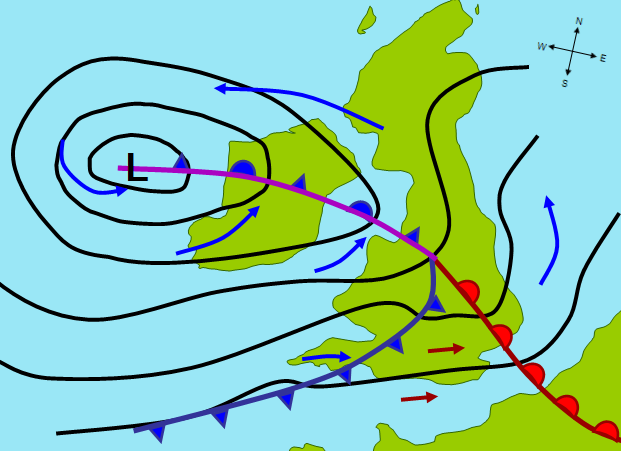
\includegraphics[width=0.4\textwidth]{isobars.png}
	\caption{Lines of constant pressure $p$ act as streamlines for the
	horizontal flow.}
	\label{fig:isobars}.
\end{figure}

In the Northern Hemisphere, air moves clockwise around high $p$ and
anticlockwise around low $p$. A \emph{cyclonic} rotation is in the same sense
as $\symbf{\Omega}$, \emph{anticyclonic} in the opposite sense as $\symbf{\Omega}$.

\subsubsection{Taylor-Proudman Theorem}
Consider an incompressible, ideal fluid in geostrophic balance (small \Ro,
\Ek)
\begin{align}
	\nabla \cdot \symbf{u} &= 0\\
	2 \symbf{\Omega} \times \symbf{u} &= -\frac{1}{\rho}\nabla p \label{tpt}
\end{align}

Taking the curl of \eqref{tpt} we have
\begin{equation}
	\begin{aligned}
		\nabla \times \left( \symbf{\Omega} \times \symbf{u}\right) &= \vare_{ijk}
		\partial_j \vare_{klm} \Omega_l u_m \\
		&= \vare_{kij} \vare_{klm} \Omega_l \partial_j u_m \\
		&= \left(\delta_{il} \delta_{jm} - \delta_{im} \delta_{jl}\right)
		\Omega_l \partial_j u_m \\
		&= \Omega_i \partial_j u_j - \Omega_j \partial_j u_i
	\end{aligned}
\end{equation}

The first term is $0$ by incompressibility. Thus
\begin{equation}
	-\nabla \times \left(\symbf{\Omega} \times \symbf{u}\right) = \symbf{\Omega} \cdot
	\nabla \symbf{u} = 0
\end{equation}

For $\symbf{\Omega} = (0, 0, \Omega)$, this implies $\frac{\partial w}{\partial
z} = 0$. If $w = 0$ on some horizontal surface (e.g. ground) then $w=0$
everywhere. 

Also, $u_x + v_y = 0$, i.e. horizontal velocity is non-divergent in
geostrophic balance. Fluid moves in `columns' parallel to $\symbf{\Omega}$,
called \emph{Taylor columns}.

\subsection{Departures from geostrophy}
Consider an incompressible, rotating fluid with constant density $\rho_0$ with
angular velocity $\symbf{\Omega} = (0, 0, f/2)$. Assume small ampltiude motions
(i.e. $\abs{\symbf{u}}^2 \ll \abs{\symbf{u}}$), i.e. neglect $\symbf{u}\cdot \nabla
\symbf{u}$ and $\nu \nabla^2 \symbf{u}$. From \eqref{nsrot},

\begin{align}
	u_t - fv &= -\frac{p_x}{\rho_0} \label{nsrot1} \\
	v_t + fu &= -\frac{p_y}{\rho_0} \label{nsrot2}\\
	w_t &= -\frac{p_z}{\rho_0} \label{nsrot3}\\
	u_x + v_y + w_z &= 0 \label{nsrot4}
\end{align}

We will eliminate variables in favour of $p$.
\begin{equation}
	\begin{aligned}
		\nabla \cdot \left( \eqref{nsrot1} - \eqref{nsrot3}\right) &\implies
\nabla^2 p = \rho_0 f\left(v_x - u_y\right) \\
\partial_x \eqref{nsrot2} - \partial_y \eqref{nsrot1} \& \eqref{nsrot4}
&\implies (v_x-u_y)_t = fw_z \\
\end{aligned}
\end{equation}

Combining these and using \eqref{nsrot3} we have
\begin{equation}
	\nabla^2 p_{tt} + f^2 p_{zz} = 0
\end{equation}
which is a wave equation for $p$. Seek plane wave solutions with ansatz 
\begin{equation}
	p = \hat{p}e^{i\left(kx + ly + mz-\omega t\right)}
\end{equation}
and dispersion relation
\begin{equation}
	\omega^2 = \frac{f^2 m^2}{k^2+l^2+m^2} = f^2 \sin^2 \theta
\end{equation}

\begin{center}
\begin{tikzpicture}
	\draw[->,thick] (-0.1,0) -- (5,0) node[below]{horizontal};
	\draw[->,thick] (0,-0.1) -- (0,3) node[left]{$z$};
	\draw[->] (0, 2.5) [partial ellipse = -180:70:0.3 and 0.1];
	\draw (0.2,2.5) node[right] {$\symbf{\Omega}$};
	\draw[->] (0,0) -- (3, 2);
	\draw (3.1, 2.1) node[right] {$\symbf{k} = (k, l, m)$};
	\draw (0.9,0) arc (0:30:1);
	\draw (1.05,0.3) node {$\theta$};
	\draw[dashed] (1.66, 2.5) -- (2.95,0.58) node[midway,right] {lines of phase};
	\draw[->,thick, red] (1.5, 2.5) -- (2.25, 3) node[right] {$\symbf{c}_p$};
	\draw[->,thick, red] (1.5,2.5) -- (1.97, 1.8) node[left] {$\symbf{c}_g$};
\end{tikzpicture}
\end{center}

This is the dispersion relation for rotating internal waves. They have phase
speed $\symbf{c}_p = w/\symbf{k}$ and group velocity 
\begin{equation}
	\symbf{c}_g = \frac{\partial w}{\partial \symbf{k}} = \pm f \frac{(-km, -lm, k^2
		+ l^2)}{\abs{\symbf{k}}^{3/2}}
\end{equation}
Note that $\symbf{c}_p\cdot\symbf{c}_g = 0$. Also note $\abs{\omega} \le \abs{f}$.

\lecture{16/10/2020}
\subsubsection{Inertial (free) oscillations}
Assume $\nabla p = \symbf{0}$.  The $x$ and $y$ components of geostrophic balance
\eqref{nsrot1}, \eqref{nsrot2} give
\begin{equation}
	u_{tt} + f^2 u = 0
\end{equation}
Thus $u = U \sin ft$ where $f$ is the \emph{inertial frequency}. Similarly, we
have $v = U \cos ft$. For a particle with position $(x_p, y_p)$ floating on an
ocean surface $z=0$ moving with the fluid velocity, we have
\begin{equation}
	\begin{aligned}
		\frac{\diffd x_p}{\diffd t} = u &\implies x_p = -\frac{U}{f} \cos ft +
		x_0 \\
		\frac{\diffd y_p}{\diffd t} = v &\implies y_p = -\frac{U}{f} \sin ft +
		y_0
	\end{aligned}
\end{equation}

Thus the motion of fluid particles describes describes \emph{inertial circles}
with radius $\frac{2U}{f}$.

\subsubsection{Ekman layer}
Look for a \emph{steady} ocean response to a constant wind stress
$\symbf{\tau}_w$. Use local Cartesian coordinates and make the following assumptions:
\begin{enumerate}
	\item Steady, i.e. $\partial_t \equiv 0$
	\item Neglect horizontal variations, i.e. $\partial_x = \partial_y = 0$
	\item Neglect surface waves, i.e. $w(z=0) = 0$
	\item No flow in deep ocean, i.e. $\lim_{z \to -\infty} \symbf{u} = \symbf{0}$
	\item Constant density $\rho$
	\item Traditional approximation
\end{enumerate}

Continuity (incompressibility) says $u_x + v_y + w_z = 0$. Assumptions $2$ and
$3$ then imply $w = 0$ everywhere. The horizontal momentum equations are
\begin{align}
	-fv &= \nu u_{zz} \label{hmom1} \\
	fu &= \nu v_{zz} \label{hmom2}
\end{align}
Define the \emph{complex velocity} $\mathcal{V} \equiv u+iv$. Then
\begin{equation}
	\mathcal{V}_{zz} = \frac{if}{\nu} \mathcal{V} \label{compvel}
\end{equation}

Without loss of generality, assume $\symbf{\tau}_w$ is aligned with the $x$-axis:
$\symbf{\tau}_w = (\tau_w, 0) = (\rho \nu u_z, 0)$. Boundary conditions for
\eqref{compvel} are
\begin{equation}
	\begin{aligned}
		\mathcal{V}_z &= \left( \frac{\tau_w}{\rho \nu}, 0\right) \hspace{1em}
		\text{at} \, \, z = 0 \\
		\mathcal{V} &= (0,0) \hspace{1em} \text{as}\,\, z \to -\infty
	\end{aligned}
\end{equation}

Thus $\mathcal{V} = Ae^{(1+i)z/\delta}$ where $\delta = \sqrt{\frac{2\nu}{f}},
A = \frac{\tau_w \delta (1-i)}{2 \rho \nu}$. In terms of the velocity
components, we have
\begin{equation}
	\begin{aligned}
		u &= \frac{\tau_w}{\rho \sqrt{\nu f}} e^{z/\delta} \cos \left(
		-\frac{z}{\delta} + \frac{\pi}{4}\right) \\
		v &= -\frac{\tau_w}{\rho \sqrt{\nu f}} e^{z/\delta} \sin \left(
		-\frac{z}{\delta} + \frac{\pi}{4}\right) \\
	\end{aligned}
\end{equation}

A top view of the ocean shows an \emph{Ekman spiral}: see
figure~\ref{fig:ekman}.
\begin{figure}
	\centering
	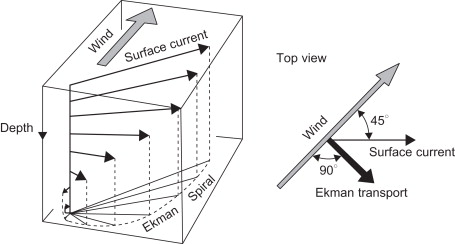
\includegraphics[width=0.5\textwidth]{ekman_spiral.jpg}
	\caption{Ekman spiral.}
	\label{fig:ekman}
\end{figure}

\subsubsection{Ekman transport}
Integrate the horizontal momentum equations \eqref{hmom1},\eqref{hmom2} to the
base of the Ekman layer where $\nu \symbf{u}_z \approx 0$ at $z=-h$. Since $\nu
\symbf{u}_z (z=0) = (\tau_w/\rho, 0)$, the \emph{Ekman transport} $\symbf{U}_T$ is
\begin{equation}
	\begin{aligned}
		U_T &\equiv \int_{-h}^0 u \, \diffd z = 0 \\
		V_T &\equiv \int_{-h}^0 v \, \diffd z = -\frac{\tau_w}{\rho f}
	\end{aligned}
\end{equation}

This is the net transport of fluid in the Ekman layer and is oriented
$90^{\circ}$ to the right of the applied wind shear stress (in the Northern
Hemisphere).

\subsubsection{Ekman pumping}
Consider a wind stress $\tau_w(y)$ that varies over large scales. Then from
incompressibility
\begin{equation}
	\int_{-h}^0 w_z \, \diffd z = -\int_{-h}^0 u_x \, \diffd z - \int_{-h}^0
	v_y \, \diffd z
\end{equation}

Thus for $h$ constant, 
\begin{equation}-w(z=-h) = -\frac{\partial V_T}{\partial y} =
\frac{\partial}{\partial y}\left( \frac{\tau_w}{\rho f}\right)
\end{equation}

In general we have
\begin{equation}
	w(z=-h) = \hat{\symbf{z}} \cdot \nabla \times \frac{\symbf{\tau}_w}{\rho f}
\end{equation}

\lecture{19/10/20}
\section{Shallow Water Systems}
\subsection{Rotating shallow water equations}
Consider a thin layer of fluid with constant density $\rho$. Define
characteristic scales
\begin{itemize}
	\item length $L = \text{horiz.}, H = \text{vert.}$
	\item velocity $U$
	\item time $T$
	\item pressure $P$
\end{itemize}
such that $\partial_x, \partial_y \sim \frac{1}{L}, \partial_z \sim
\frac{1}{H}$. Define the \emph{aspect ratio} $\delta \equiv H/L$. We will
assume $\delta \ll 1$. From continuity (incompressibility) we have
\begin{equation}
	\begin{aligned}
		\frac{\partial w}{\partial z} &= -\frac{\partial u}{\partial x} -
		\frac{\partial v}{\partial y}  \\
		\implies \frac{w}{H} &= \mathcal{O}(U/L) \\
		\implies w &= \mathcal{O}(\delta U)
	\end{aligned}
\end{equation}

Using the traditional approximation and assuming the fluid is inviscid, the
$x$-momentum equation
\begin{align}
	&\frac{\partial u}{\partial t} &&+ u \frac{\partial u}{\partial x} &&+v
	\frac{\partial u}{\partial y} &&+ w\frac{\partial u}{\partial z} &&- fv &&=
						&&-\frac{1}{\rho} \frac{\partial p}{\partial x}
	\label{eq:swxmom}\\
	\text{scaling:}\hspace{1em} &\frac{U}{T} &&\frac{U^2}{L} && \frac{U^2}{L}
					&&\frac{wU}{H} &&fU &&= &&\frac{P}{\rho L}
\end{align}

Thus if $p_x$ appears at leading order then
\begin{equation}
	P \sim \rho U \max(L/T, U, fL)
\end{equation}

Similarly the $z$-momentum equation and its scalings are
\begin{align}
	&\frac{\partial w}{\partial t} &&+ u \frac{\partial w}{\partial x} &&+v
	\frac{\partial w}{\partial y} &&+ w\frac{\partial w}{\partial z} &&=
						&&-\frac{1}{\rho} \frac{\partial p}{\partial x} - g
	\label{eq:swzmom} \\
	\text{scaling:}\hspace{1em} &\frac{w}{T} &&\frac{Uw}{L} && \frac{Uw}{L}
					&&\frac{w^2}{H} &&= &&\frac{P}{\rho H}
\end{align}

Hence $\frac{\diffD w}{\diffD t} \sim \max(\frac{w}{T}, \frac{Uw}{L})$. Comparing with the
pressure term, we have
\begin{align}
	\frac{\frac{\diffD w}{\diffD t}}{\frac{1}{\rho}\frac{\partial p}{\partial
		z}} &\sim \frac{\max(\frac{w}{T},
		\frac{Uw}{L})}{\frac{U}{H}\max(\frac{L}{T}, \frac{U}{L}, f)}\\
		&\sim \delta^2
		\frac{\max(\frac{1}{T},\frac{U}{L})}{\max(\frac{1}{T},\frac{U}{L},f)}
\end{align}

Therefore to $\mathcal{O}(\delta^2)$ we have \emph{hydrostatic balance}. To
this order, \eqref{eq:swzmom} becomes
\begin{equation}
	\frac{\partial p}{\partial z} - \rho g \implies p = \rho g (\eta - z)
\end{equation}
assuming $p = 0$ at $z = \eta(x,y,t)$. Similarly, we have $\frac{1}{\rho} p_x
= g \eta_x$ and $\frac{1}{\rho} p_y = g \eta_y$. Hence horizontal acceleration
(i.e. the LHS of \eqref{eq:swxmom}) is independent of $z$. Motivated by this,
we \emph{assume} that horizontal velocity is also independent of $z$. For $\Ro
\ll 1$, this follows from the Tayor-Proudman theorem.

Re-writing \eqref{eq:swxmom} with these results we have
\begin{align}
	u_t + u u_x + v u_y -fv &= -g \eta_x \label{eq:swx}\\
	v_t + u v_x + v v_y + fu &= -g \eta_y \label{eq:swy}
\end{align}
since $u_z = v_z = 0$ by assumption. Integrating the continuity equation gives
\begin{equation}
	w = -z(u_x + v_y) + A(x,y,t)
\end{equation}
where $A$ is to be determined by the boundary conditions. Requiring no normal
flow at $z = -H_0 + h_b$ is imposed by $\symbf{u}\cdot\hat{\symbf{n}} = 0$ where
$\symbf{n} = \nabla(z-h_b)$. Thus
\begin{equation}
	-u\frac{\partial h_b}{\partial x} -v \frac{\partial h_b}{\partial y} + w = 0
\end{equation}

Hence
\begin{equation}
	A(x,y,t) = u \frac{\partial h_b}{\partial x} + v \frac{\partial
	h_b}{\partial y} + (-H_0 + h_b) (u_x+v_y)
\end{equation}

The kinematic boundary condition at $z = \eta$ is $\frac{\diffD \eta}{\diffD
t} = w$ which may be written as
\begin{equation}
	\eta_t + u \eta_x + v \eta_y - w = 0
\end{equation}
where $w = -\eta(u_x+v_y) + u \frac{\partial h_b}{\partial x} + v
\frac{\partial h_b}{\partial y} + (-H_0 + h_b)(u_x+v_y)$. Combining these
boundary conditions gives
\begin{equation}
	\eta_t + \left[ (H_0-h_b+\eta)u\right]_x + \left[ (H_0-h_b+\eta)v\right]_y
	= 0 \label{eq:swcon}
\end{equation}
If $H \equiv H_0 - h_b + \eta$ is the total depth of the fluid, then since
$H_t = \eta_t$,
\begin{equation}
	H_t + (uH)_x + (vH)_y = 0 \label{eq:swcon2}
\end{equation}
which is a statement of the conservation of volume (equivalently mass, since
$\rho$ is constant). Equations \eqref{eq:swx}, \eqref{eq:swy}, and
\eqref{eq:swcon} are the \emph{rotating shallow water} (SW) equations.

\subsubsection{Potential vorticity (PV)}
Denote the vertical vorticity by $\zeta = v_x - u_y$. Consider $\partial_x
\eqref{eq:swy} - \partial_y \eqref{eq:swx}$, which gives
\begin{equation}
	\zeta_t +u\zeta_x + v\zeta_y + v f_y = -(\zeta + f)(u_x+v_y)
\end{equation}
Now from conservation of volume \eqref{eq:swcon2},
\begin{equation} 
	u_x + v_y = -\frac{1}{H} \frac{\diffD H}{\diffD t}
\end{equation}
Combining these relates the material derivative of $\zeta$ and $H$ by
\begin{equation}
	\frac{\diffD \zeta}{\diffD t} + \frac{\diffD f}{\diffD t}= \frac{\zeta + f}{H} \frac{\diffD H}{\diffD
	t} \implies \frac{\diffD}{\diffD t}\left(\frac{\zeta + f}{H}\right) = 0
	\label{eq:PV}
\end{equation}

Let $q \equiv \frac{\zeta + f}{H}$, the \emph{shallow water potential
vorticity} (SWPV). SWPV is conserved following fluid motion. We call $\zeta$
the \emph{relative vorticity} and $f$ the \emph{planetary vorticity}. $\zeta$
and $f$ will change as a fluid moves to conserve SWPV (changing $f$) and
angular momentum (changing depth).

\begin{center}
\begin{tikzpicture}
	\draw[thick,->] (0,2.5) -- (0, 3.5);
	\draw[->] (0, 3) [partial ellipse = -180:70:0.4 and 0.12];
	\draw (0.5, 2.8) node {$\symbf{\Omega}$};
	\draw[thick, smooth,domain=-3:3] plot({\x}, {1/(1+exp(3*\x))});
	\draw[thick, smooth,domain=-3:3] plot({\x}, {2});
	\draw (3,2) node[right] {$z=0$};
	\draw (3,0) node[right] {$z=-H$};
	\draw[blue] (-2,0.998) -- (-2,2);
	\draw[blue] (-1,0.953) -- (-1,2);
	\draw[blue] (1.5,0.011) -- (1.5, 2);
	\draw[blue] (2,0.002) -- (2,2);
	\draw[thick,blue,->] (1.75, 1) [partial ellipse = -180:70:0.4 and 0.12];
	\draw[thick, blue,->] (-1.5, 1.5) [partial ellipse = -180:70:0.7 and 0.2];
	\draw[red, thick, ->] (-0.25,1.25) -- (0.75, 1.25) node[midway,above]
		{$\zeta, H \symbf{u}parrow$};
\end{tikzpicture}
\qquad
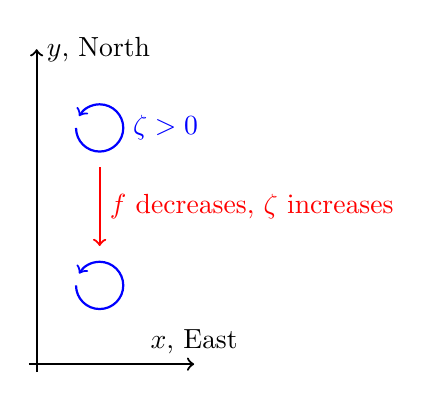
\begin{tikzpicture}
	\draw[thick,->] (-0.1,0) -- (2, 0) node[above] {$x$, East};
	\draw[thick,->] (0,-0.1) -- (0, 4) node[right] {$y$, North};
	\draw[thick,blue,->] (0.5, 3) arc(-180:150:0.3);
	\draw[thick,blue,->] (0.5, 1) arc(-180:150:0.3);
	\draw[thick,red,->] (0.8, 2.5) -- (0.8, 1.5) node[midway,right] {$f$
		decreases, $\zeta$ increases};
	\draw[blue] (1.1, 3) node[right] {$\zeta > 0$};
\end{tikzpicture}
\end{center}

\lecture{21/10/20}
\subsection{Small amplitude motions in rotating SW}
Consider a stationary fluid with depth $H_s(x,y) = H_0 - h_b$. The fluid
surface is then perturbed by $\eta(x,y,t)$ where $\eta \ll H_s$. The total
depth is $H(x,y,t) = H_s + \eta$. For $\abs{\symbf{u}}^2 \ll \abs{\symbf{u}}$,
linearise the shallow water equations:
\begin{align}
	u_t - fv &= -g \eta_x \label{swlin1} \\
	v_t + fu &= -g \eta_y \label{swlin2}\\
	\eta_t + (uH_s)_x + (vH_s)_y &= 0 \label{swlin3}
\end{align}

Assuming $f$ is constant, we have from $\partial_x \eqref{swlin1} + \partial_y
\eqref{swlin2}$ and $\partial_y \eqref{swlin1} - \partial_x \eqref{swlin2}$:
\begin{equation}
	\partial_t \left[ \left(\partial_t^2 + f^2\right) \eta - \nabla
		\cdot\left(gH_s \nabla \eta \right)\right] - fg J(H_s, \eta) = 0
		\label{swlin6}
\end{equation}
where the Jacobian $J(a,b) = a_x b_y - a_y b_x$. For the velocity components
we have
\begin{align}
	\left( \partial_t^2 + f^2\right)u &= -g\left( \eta_{xt} + f\eta_y\right)
	\label{swlin4}\\
	\left( \partial_t^2 + f^2\right)v &= -g\left( \eta_{yt} +
	f\eta_x\right)\label{swlin5}
\end{align}

\subsubsection{Steady flows}
We now assume $\partial_t = 0$. From \eqref{swlin4}, \eqref{swlin5},
\begin{equation}
	u = -\frac{g}{f}\eta_y, \hspace{2em} v = \frac{g}{f}\eta_x
\end{equation}
This is \emph{shallow water geostrophic balance}: the surface displacement
$\eta$ acts as a streamfunction. Applying the steady assumption to
\eqref{swlin6} gives $J(H_s, \eta) = 0$ which implies $\eta = \eta(H_s(x,y))$.
Hence linearised steady geostrophic flow in shallow water follows contours of
constant depth.  Steady PV conservation follows from \eqref{eq:PV} with
$\partial_t = 0$ and assuming $\zeta \ll f$
\begin{equation}
	\symbf{u} \cdot \nabla \frac{f}{H_s} = 0
\end{equation}
Thus when $f$ varies, the flow follows contours of constant $f/H_s$.

\subsubsection{Waves in an unbounded domain}
Assume $H_s$ is constant. From \eqref{swlin6}, we have
\begin{equation}
	\left( \partial_t^2 + f^2\right)\eta - gH_s \nabla^2 \eta = 0
\end{equation}

Seek plane wave solutions to this wave equation with ansatz $\eta = \eta_0
\exp(i(kx+ly-\omega t))$. The dispersion relation is then
\begin{equation}
	\omega^2 = f^2 + gH_s (k^2 + l^2) \label{eq:poindisp}
\end{equation}

If $f = 0$, i.e. no rotation, then the frequency is $\omega = \pm \sqrt{gH_s}
\abs{\symbf{k}} = \omega_0$ and the phase speed is $\abs{c_p} =
\frac{\abs{\omega}}{\abs{\symbf{k}}} = \sqrt{gH_s} = c_0$. For $f \ne 0$, we get
\emph{Poincar\'{e}} waves with
\begin{equation}
	\omega^2 > \omega_0^2, \hspace{2em} \abs{c_p} > c_0
\end{equation}
i.e. rotation increases the frequency and phase speed. Define the \emph{Rossby
deformation scale} $R_D \equiv \frac{c_0}{f}$. From \eqref{eq:poindisp},
\begin{equation}
	\frac{\omega^2}{f^2} = 1 + R^2_D \abs{\symbf{k}}^2
\end{equation}

Without loss of generality, let $l = 0$, by reorienting $x$ and $y$. If $\eta
= \eta_0 \cos(kx-\omega t)$ then \eqref{swlin4}, \eqref{swlin5} imply the
fluid velocity is
\begin{align}
	u &= \frac{\omega_0 \eta_0}{k H_s} \cos(kx-\omega t) \\
	v &= \frac{f \eta_0}{k H_s}
\end{align}
Thus the motion is an ellipse, also known as a \emph{tidal ellipse}, which
reduces to intertial circles if $\omega_0 = f$:
\begin{equation}
	u^2 + \frac{\omega_0^2}{f^2} v^2 = \frac{\omega_0^2 \eta_0^2}{k^2 H_s^2}
\end{equation}
Since $\omega > f$, the fluid moves anticylonically. The Rossby deformation
scale $R_D$ is the length scale for which rotation becomes important. Consider
short and long waves:
\begin{itemize}
	\item Short waves: $\abs{\symbf{k}} R_D \gg 1$. We have $\omega^2 \to g H_s
		\abs{\symbf{k}}^2$ i.e. non-rotating shallow water gravity waves.
	\item Long waves: $\abs{\symbf{k}}R_D \ll 1$. We have $\omega^2 \to f^2$ i.e.
		inertial waves where fluid moves in inertial circles. Gravity is not
		involved.
\end{itemize}

\lecture{23/10/20}
\subsection{Geostrophic adjustment}
Consider the response of rotating shallow water to an initial state \emph{not}
in geostrophic balance. Here, we consider $\eta(x,y,) = \eta_0 \sgn(x)$,
$\symbf{u}(x,y,0) = \symbf{0}$, so the initial PV is $0$. 


Assume $f$ is constant, the perturbation is small $\eta_0 \ll H$, the PV is
small $\zeta \ll f$, and the bottom is flat $H_s = H_0$. Linearise the shallow
water PV:
\begin{equation}
	q = \frac{f+\zeta}{H_0+\eta} = \frac{f}{H_0}\left(1+\frac{\zeta}{f} +
		\dots\right)\left(1-\frac{\eta}{H_0}+\dots\right) \approx
		\frac{f}{H_0}\left(1+\frac{\zeta}{f} - \frac{\eta}{H_0}\right)
\end{equation}

Since PV is conserved, we have
\begin{equation}
	\frac{\zeta}{f} - \frac{\eta}{H_0} = -\frac{\eta_0}{H_0} \sgn(x)
	\hspace{2em} \forall t \label{eq:PVcons}
\end{equation}

By symmetry, $\partial_y \equiv 0$ so the PV is $\zeta = v_x$. The linearised
shallow water equations in this case
\begin{align}
	u_t - fv &= -g\eta_x \\
	v_t + fu &= 0 \\
	\eta_t + H_0 u_x &= 0
\end{align}

Using these equations we have
\begin{equation}
	\zeta = v_x = \frac{u_{xt} + g\eta_{xx}}{f} = -\frac{1}{f H_0} \eta_{tt} +
	\frac{g}{f}\eta_{xx}
\end{equation}

Now conservation of potential vorticity \eqref{eq:PVcons} gives
\begin{equation}
	\eta_{tt} - c^2 \eta_{xx} + f^2 \eta = f^2 \eta_0 \sgn(x)
\end{equation}
where $c^2 \equiv g H_0$. This is a \emph{Klein-Gordon equation} where the
$f^2\eta$ term adds elasticity to the waves.

\subsubsection{Steady solutions}
Consider steady solutions. Owing to the step forcing, our BCs are to match
$\eta_x$ and $\eta$ at $x=0$. We find
\begin{equation}
	\eta = \eta_0 \begin{cases} 1 - e^{-x/R_d} & x > 0 \\ -1 + e^{x/R_d} & x <
	0 \end{cases} \label{eq:gasoln}
\end{equation}
where $R_d \equiv \sqrt{gH_0}/f$ is the \emph{deformation radius}. From the
equations of geotrophic balance we have the velocity components
\begin{equation}
	u = 0, \hspace{2em} v = \frac{g \eta_0}{fR_d} e^{-\abs{x}/R_d}
\end{equation}
\begin{center}
	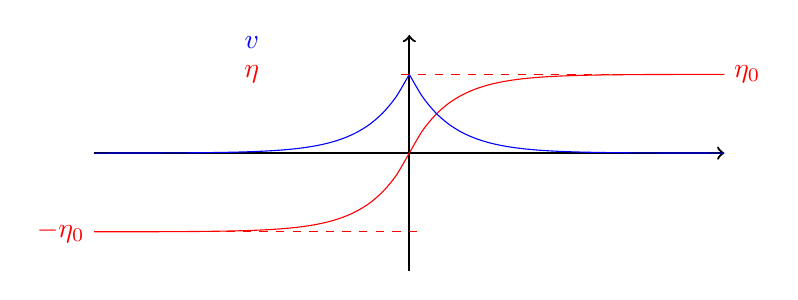
\begin{tikzpicture}
		\draw[thick,->] (-4,0) -- (4,0);
		\draw[thick,->] (0,-1.5) -- (0,1.5);
		\draw[smooth,domain=0:4,red] plot({\x},{1-exp(-2*\x)});
		\draw[smooth,domain=-4:0,red] plot({\x},{-1+exp(2*\x)});
		\draw[smooth,domain=0:4,blue] plot({\x},{exp(-2*\x)});
		\draw[smooth,domain=-4:0,blue] plot({\x},{exp(2*\x)});
		\draw[red,dashed] (-0.1,1) -- (4, 1) node[right] {$\eta_0$};
		\draw[red,dashed] (0.1,-1) -- (-4, -1) node[left] {$-\eta_0$};
		\draw[red] (-2, 1) node {$\eta$};
		\draw[blue] (-2, 1.4) node {$v$};
	\end{tikzpicture}
\end{center}

\subsubsection{Transients}

The steady solution \eqref{eq:gasoln} solves the geostrophic adjustment
equation, but it does not match the initial conditions. We add this particular
solution to a solution to the homogeneous equation
\begin{equation}
	\eta_{tt} - c^2 \eta_{xx} + f^2 \eta = 0
\end{equation}
with initial condition
\begin{equation}
	\eta = \eta_0 \sgn(x) - \eta_{\text{steady}} = \eta_0
	e^{-\abs{x}/R_d}\sgn(x)
\end{equation}

We seek solutions of plane wave form
\begin{equation}
	\eta = \hat{\eta} e^{i(kx-\omega t)}
\end{equation}
with $\omega^2 = f^2 + c^2 k^2$. These are Poincar\'{e} waves.

\subsubsection{Energetics}
The change in potential energy per unit length in the $y$ direction is
\begin{align}
	PE_{\text{initial}} - PE_{\text{final}} &= \int_{-\infty}^\infty
	\int_0^{\eta_i} \rho_0 g z \, \diffd z \, \diffd x - \int_{-\infty}^\infty
	\rho_0 g z \, \diffd z\,\diffd x \\
	&= 2\rho_0 g \left[ \int_0^\infty \frac{\eta_i^2}{2}\,\diffd x -
\int_0^\infty \frac{\eta_f^2}{2}\,\diffd x \right] \\
&= \rho_0 g \eta_0^2 \int_0^\infty \left[ 1- (1-e^{-x/R_d})^2\right] \, \diffd
x\\
&= \frac{3}{2}\rho_0 g \eta_0^2 R_d
\end{align}

The change in kinetic energy per unit length in the $y$ direction is
\begin{align}
	KE_{\text{initial}} - KE_{\text{final}} &= \int_{-\infty}^\infty
	\int_{-H}^{\eta_i} \frac{1}{2} \rho_0 v_i^2 \,\diffd z\, \diffd x -
	\int_{-\infty}^\infty \int_{-H}^{\eta_f} \frac{1}{2} \rho_0 v_f^2 \,\diffd
	z\, \diffd x \\
	&\approx 0 - \frac{1}{2}\rho_0 \int_{-\infty}^\infty H_s v^2_f \, \diffd x
	\\
	&= -\rho_0 H_s \int_0^\infty \frac{g^2 \eta_0^2}{f^2 R_d^2} e^{-2x/R_d} \,
	\diffd x \\
	&= -\rho_0 \frac{R_d^2 g \eta_0^2}{R_d^2}\cdot -\frac{R_d}{2} \cdot \left[
e^{-2x/R_d} \right]_0^\infty \\
&= -\rho_0 g \eta_0^2 \frac{R_d}{2}
\end{align}
Only $\frac{1}{3}$ of the potential energy released is converted into kinetic
energy of the geostrophic flow. The remainder is radiated away by Poincar\'{e}
waves.

\lecture{26/10/20}
\subsection{Quasi-geostrophic equations}
Large scale motions in the ocean and atmosphere are associated with small
Rossby number $\Ro \equiv \frac{U}{fL} \ll 1$. In this limit, the rotating
shallow water equations are approximated by the SW quasi-geostrophic (SW QG)
equation. Start from the SW PV equation:
\begin{equation}
	\frac{\diffD}{\diffD t}\left(\frac{\zeta + f}{H}\right) =
	0\label{eq:PVcons2}
\end{equation}

\paragraph{Assumption 1: $\Ro \ll 1$}
Assuming a small Rossby number implies the flow is close to geostrophic
balance with
\begin{equation}
	f \symbf{\hat{k}} \times \symbf{u} \approx -g \nabla \eta
\end{equation}
where $\hat{\symbf{k}}$ is the vertical unit vector. Define the \emph{geostrophic
streamfunction} $\psi \equiv \frac{g \eta}{f}$. In terms of this
streamfunction we have
\begin{align}
	\symbf{u} &\approx - \nabla \times (\psi \hat{\symbf{k}}) \\
	\zeta &= (\nabla \times \symbf{u})\hat{\symbf{k}} \approx \nabla^2 \psi
\end{align}

\paragraph{Assumption 2: small changes in $f$}
Recall the Coriolis parameter $f = 2 \Omega \sin \theta$ where $\theta$ is
latitude. Expand in a Taylor series about $\theta = \theta_0$ to get
\begin{equation}
	f = f_0 + y \frac{\diffd f}{\diffd y}\vert_{\theta_0} + \dots \approx f_0
	+ \beta y
\end{equation}
where $y$ is in the direction of local North, $f_0 = 2\Omega \sin \theta_0$
and $\beta$ is defined as
\begin{equation}
	\beta = \frac{1}{R} \frac{\diffd f}{\diffd \theta}\vert_{\theta_0} =
\frac{2\Omega}{R} \cos \theta_0\end{equation}
with $R$ the radius of Earth. For characteristic length scale $L$, assume
$\frac{\beta L}{f_0} \ll 1$. This is the \emph{$\beta$-plane approximation}.

\paragraph{Assumption 3: small changes in fluid height.}
This is consistent with small Rossby number: from geostrophic balance, we know
$\eta \sim \frac{f UL}{g}$ and $\frac{\eta}{H_0} \sim \frac{fUL}{gH_0} =
\frac{U}{fL} \frac{L^2}{R_D^2}$. Therefore $\eta/H_0 \ll 1$ if $\Ro \ll
\frac{R^2_D}{L^2}$. For $L \sim R_D$, $\Ro \ll 1$ implies $\eta/H_0 \ll 1$.
Further, we assume $h_b/H_0 \ll 1$. 

\paragraph{Quasi-geostrophic equations.} With these assumptions, SWPV becomes
\begin{align}
	\frac{\zeta + f}{H_0 - h_b + \eta} &\approx \frac{f_0}{H_0} \frac{1+
		\frac{\beta y}{f_0} + \frac{\zeta}{f_0}}{1 - \frac{h_b}{H_0} +
	\frac{\eta}{H_0}} \\
	&\approx \frac{f_0}{H_0} \left(1+\frac{\beta y}{f_0} + \frac{\nabla^2
\psi}{f_0} + \frac{h_b}{H_0} - \frac{f_0 \psi}{g H_0}\right) \\
&= \frac{f_0}{H_0} P_g
\end{align}
where $P_g$ is the \emph{quasi-geostrophic potential vorticity} and $\zeta =
\nabla^2 \psi, \eta = \frac{f_0 \psi}{g}$. Hence from SWPV conservation
\eqref{eq:PVcons2},
\begin{equation}
	\frac{\partial P_g}{\partial t} + \symbf{u} \cdot \nabla P_g \approx 0
\end{equation}

Using $\symbf{u} \approx - \nabla \times (\psi \hat{\symbf{k}})$, $\symbf{u} = -\psi_y,
v = \psi_x$ so
\begin{equation}
	\frac{\partial P_g}{\partial t} + J(\psi,P_g) \approx 0\label{eq:swqg}
\end{equation}
This is the \emph{shallow water Quasi-geostrophic} (SWQG) equation, which is
one equaiton for one unknown $\psi$, as opposed to SWPV with 2 unknowns
$\zeta, \eta$.

\subsubsection{Waves in QG}
Assume a flat bottom $h_b = 0$. Linearise \eqref{eq:swqg} about a state of
rest (i.e. neglect terms $\mathcal{O}(\psi^2)$). Then
\begin{equation}
	\frac{\partial}{\partial t} \left( \nabla^2 \psi - \frac{f_0^2}{gH_0}
	\psi\right) + \frac{\partial \psi}{\partial x}\beta = 0
\end{equation}
Seek plane wave solutions of the form
\begin{equation}
	\psi = \psi_0 e^{i(kx + ly - \omega t)}
\end{equation}
with dispersion relation
\begin{equation}
	\omega = \frac{-k \beta}{k^2 + l^2 + R_D^{-2}}, \hspace{2em} R_D \equiv
	\frac{\sqrt{gH_0}}{f_0}
\end{equation}
This is the \emph{Rossby wave dispersion relation}. Note $\omega = 0$ (i.e. no
waves) if $\beta = 0$. Also, if $h_b = 0$ and $\beta = 0$ there are no wave
solutions unlike rotating SW. Thus the QG system `filters' out Poincar\'{e}
waves. Note that $\beta = \frac{2 \Omega}{R} \cos \theta \ge 0$, hence $c_p =
\frac{\omega}{k} \le 0$. Rossby wave speed is always directed to the
\emph{west}.

Consider the size of the dynamic terms in $P_g$, specifically the ratio of
relative vorticity to surface height
\begin{equation}
	\frac{\nabla^2 \psi}{-\frac{f_0^2 \psi}{g H_0}} \sim \frac{R_D^2}{L^2}
\end{equation}

Hence relativity vorticity dominates at scales small compared to $R_D$ whilst
surface height dominates at scales large compared to $R_D$.

\subsubsection{Physical interpretation of Rossby waves}
Consider $L \ll R_d$ ($L \gg R_D$)  and a small perturbation in the dominant
term for the scale, $\zeta$ ($\eta$). For $L \ll R_D$, the planetary vorticity
increases (thus $\zeta$ decreases) on the westward side, whilst the planetary
vorticity decreases (thus $\zeta$ increases) on the eastward side. Hence the
perturbation propagates westwards. For $L \gg R_D$, the planetary vorticity
increases ($\eta$ increases) on the westward size and decreases ($\eta$
decreases) on the eastward side as before. Thus the perturbation propagates
to the west also. These are Rossby waves.
\begin{center}
	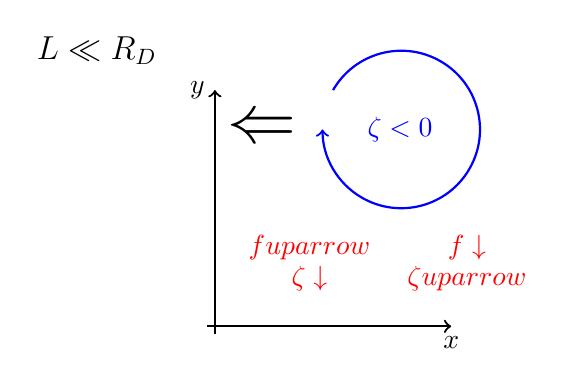
\begin{tikzpicture}
		\draw (-1.5, 3.5) node {\large $L \ll R_D$};
		\draw[thick,->] (-0.1, 0) -- (3, 0) node[below] {$x$};
		\draw[thick,->] (0, -0.1) -- (0, 3) node[left] {$y$};
		\draw[thick,blue,->] (1.5, 3) arc(150:-180:1);
		\draw[blue] (2.35, 2.5) node {$\zeta < 0$};
		\draw[red] (1.2, 1) node {$f \symbf{u}parrow$};
		\draw[red] (1.2, 0.6) node {$\zeta \downarrow$};
		\draw[red] (3.2, 1) node {$f \downarrow$};
		\draw[red] (3.2, 0.6) node {$\zeta \symbf{u}parrow$};
		\draw[thick] (0.6, 2.5) node {\Huge$\Leftarrow$};
	\end{tikzpicture}
	\qquad
	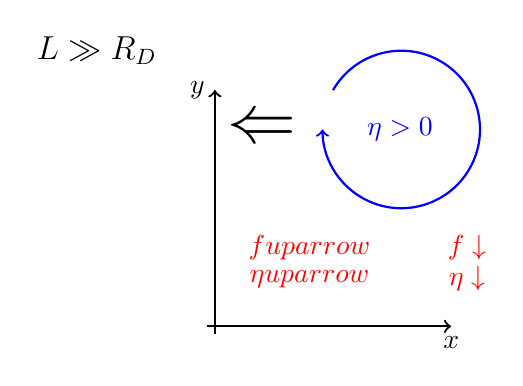
\begin{tikzpicture}
		\draw (-1.5, 3.5) node {\large $L \gg R_D$};
		\draw[thick,->] (-0.1, 0) -- (3, 0) node[below] {$x$};
		\draw[thick,->] (0, -0.1) -- (0, 3) node[left] {$y$};
		\draw[thick,blue,->] (1.5, 3) arc(150:-180:1);
		\draw[blue] (2.35, 2.5) node {$\eta > 0$};
		\draw[red] (1.2, 1) node {$f \symbf{u}parrow$};
		\draw[red] (1.2, 0.6) node {$\eta \symbf{u}parrow$};
		\draw[red] (3.2, 1) node {$f \downarrow$};
		\draw[red] (3.2, 0.6) node {$\eta \downarrow$};
		\draw[thick] (0.6, 2.5) node {\Huge$\Leftarrow$};
	\end{tikzpicture}
\end{center}

\subsection{Large scale ocean circulation}
\subsubsection{Sverdrup flow}
Seek steady solutions for rotating shallow water driven by a wind stress
$\symbf{\tau}_w$. We have
\begin{align}
	\frac{\diffD \symbf{u}}{\diffD t} + f \hat{\symbf{k}}\times\symbf{u} &= -g \nabla \eta +
	\frac{\symbf{\tau}_w}{\rho H} \label{eq:lsoc1} \\
	H_t + \nabla \cdot (\symbf{u} H) &= 0 \label{eq:lsoc2}
\end{align}

Consider $\nabla \times \eqref{eq:lsoc1} \cdot \hat{\symbf{k}}$ and
\eqref{eq:lsoc2} which implies modified PV conservation
\begin{equation}
	\frac{\diffD}{\diffD t} \left( \frac{\zeta + f}{H}\right) = \frac{1}{H}
	\nabla \times \left( \frac{\symbf{\tau}_w}{\rho H} \right) \cdot
	\hat{\symbf{k}} \label{eq:lsocPV}
\end{equation}

Thus we see frictional forcing modifies PV conservation. Assuming $H$ is
constant, $\zeta \ll f$ ($\Ro \ll 1$), and using the $\beta$-plane
approximation $f = f_0 + \beta y$, \eqref{eq:lsocPV} becomes
\begin{equation}
	\beta v = \frac{1}{\rho H} \left(\nabla \times \symbf{\tau}_w\right) \cdot
	\hat{\symbf{k}}\label{eq:sb}
\end{equation}
This is called \emph{Sverdrup balance}. Physically, the North/South advection
of planetary vorticity $\symbf{u}\cdot\nabla f$ balances the vorticity input by
wind.

\subsubsection{Western boundary currents}
Consider steady circulation in a rectangular basin, driven by a wind stress
curl
\begin{equation}
	w(y) = \frac{\left(\nabla \times \symbf{\tau}_w\right)\cdot\hat{\symbf{k}}}{\rho
	H} \label{eq:wbc1}
\end{equation}

\begin{center}
	\begin{tikzpicture}[scale=1.5]
		\draw (0,0) -- (5,0) -- (5,3) -- (0, 3) -- (0,0);
		\draw[thick,->] (0,0) -- (0, 1) node[left] {$y$};
		\draw[thick,->] (0,0) -- (1, 0) node[below] {$x$};
		\draw[thick, red, ->] (2, 2.8) -- (3, 2.8);
		\draw[thick, red, ->] (2, 2.7) -- (3, 2.7);
		\draw[red] (2.5, 2.55) node {westerlies};
		\draw[thick, red, <-] (2, 0.2) -- (3, 0.2);
		\draw[thick, red, <-] (2, 0.3) -- (3, 0.3);
		\draw[red] (2.5, 0.45) node {trade winds};
		\draw[thick,->] (6,0) -- (8,0) node[right] {$w(y)$};
		\draw[smooth,red] plot[domain=0:3,variable=\y] ({7-(9/8)+0.5*(\y-1.5)*(\y-1.5)},{\y});
		\draw[thick,->] (7,0) -- (7, 3.5) node[right] {$y$};
		\draw[blue,->] (2, 1.7) -- (2, 1.3);
		\draw[blue,->] (2.5, 1.7) -- (2.5, 1.3);
		\draw[blue,->] (3, 1.7) -- (3, 1.3);
		\draw[blue,->] (1.5, 1.2) arc(0:-180:0.5);
		\draw[blue,->] (3.5, 1.2) arc(-180:0:0.5);
		\draw[blue] (1,1.2) node {?};
		\draw[blue] (4,1.2) node {?};
	\end{tikzpicture}
\end{center}

From \eqref{eq:sb}, $w < 0 \implies v < 0$. Recall $\symbf{u} = -\nabla \times \psi
\hat{\symbf{k}}$. Boundary conditions are no normal flow at the boundaries, i.e.
$\psi$ is constant. Sverdrup balance \eqref{eq:sb} $\beta \psi_x = w(y)$ gives
\begin{equation}
	\psi = \frac{xw(y)}{\beta} + G(y)
\end{equation}
for some arbitary function $G(y)$. This presents a problem: we cannot meet the
boundary conditions at both $x=0$ and $x=L$. Hence we need extra terms and
boundary layers. Following Musk, we include horizontal friction in
\eqref{eq:lsoc1}:
\begin{equation}
	\frac{\diffD \symbf{u}}{\diffD t} + f \hat{\symbf{k}}\times\symbf{u} = -g \nabla \eta +
	\frac{\symbf{\tau}_w}{\rho H} + \nu \nabla^2 \symbf{u} \label{eq:wbc2}
\end{equation}
Note here we are using the horizontal gradient $\nabla \equiv (\partial_x,
\partial_y)$. Consider $\nabla \times \eqref{eq:wbc2} \cdot \hat{\symbf{k}}$ with
$\zeta \ll f$. Then
\begin{equation}
	\beta \psi_x = w(y) + \nu \nabla^4 \psi\label{eq:wbcODE}
\end{equation}
The PDE is now fourth order, so we need four boundary conditions.

\begin{center}
	\begin{tikzpicture}[scale=2]
		\draw (0,0) -- (5,0) -- (5,3) -- (0, 3) -- (0,0);
		\draw[thick,->] (0,0) -- (0, 1) node[left] {$y$};
		\draw[thick,->] (0,0) -- (1, 0) node[below] {$x$};
		\draw[dashed,blue] (0.8,0) -- (0.8, 3);
		\draw[dashed,blue] (4.2,0) -- (4.2, 3);
		\draw (2.5, 1.5) node {Interior $\psi = \psi_I$};
		\draw (0.4, 1.5) node {\small Region I};
		\draw (4.6, 1.5) node {\small Region II};
		\draw (-0.5, 1.6) node {$\psi = 0$};
		\draw (-0.5, 1.4) node {$\psi_x = 0$};
		\draw (5.5, 1.6) node {$\psi = 0$};
		\draw (5.5, 1.4) node {$\psi_x = 0$};
		\draw (2.5, 3.2) node {$\psi=0, \psi_y = 0$};
		\draw (2.5, -0.2) node {$\psi=0, \psi_y = 0$};
	\end{tikzpicture}
\end{center}

In region I we have $\psi \approx \psi_I + \psi^{(1)}$ and in region II we
have $\psi \approx \psi_I + \psi^{(2)}$. The full solution is $\psi = \psi_I +
\psi^{(1)} + \psi^{(2)}$ with interior flow $\psi_I = x\frac{w(y)}{\beta} +
G(y)$.

\lecture{30/10/20}
\paragraph{Region I.} Let $\varepsilon = \nu$ with $\vare \ll 1$. Define a
rescaled coordinate $\tilde{x} \equiv \frac{x}{\vare^a}$ with $\partial_x =
\vare^{-a}\partial_{\tilde{x}}$. Note: if $a > 0$ then $\partial_x \gg
\partial_y$. This is the \emph{method of undetermined coefficients}. From the
PDE \eqref{eq:wbcODE} for $\psi$ we have
\begin{equation}
	\cancel{\beta \psi_x^I} + \beta \vare^{-a} \tilde{\psi}_{\tilde{x}}^{(1)}
	= \vare^{1-4a} \tilde{\psi}^{(1)}_{\tilde{x}\tilde{x}\tilde{x}\tilde{x}}
	+ \cancel{w} 
\end{equation}
Matching exponents, we have $a = \frac{1}{3}$. Hence 
\begin{equation}
	\beta \tilde{\psi}_{\tilde{x}}^{(1)} =
	\tilde{\psi}^{(1)}_{\tilde{x}\tilde{x}\tilde{x}\tilde{x}}\label{eq:wbcODE2}
\end{equation}

Seek solutions of the form $\tilde{\psi} = \tilde{\psi}_0 e^{r\tilde{x}}$.
Then $r^4 - \beta r = 0$ so $r =0, \beta^{1/3}, -\frac{1}{2}\beta^{1/3} \pm
i\frac{\sqrt{3}}{2}\beta^{1/3}$. The general solution is therefore
\begin{equation}
	\tilde{\psi}^{(1)} = A(y) + B(y)e^{\beta^{1/3} \tilde{x}} +
	C(y)e^{-\beta^{1/3}\frac{\tilde{x}}{2}}e^{i\frac{\sqrt{3}}{2}\beta^{1/3}\tilde{x}}
	+ D(y)e^{-\beta^{1/3}\frac{\tilde{x}}{2}}e^{-i\frac{\sqrt{3}}{2}\beta^{1/3}\tilde{x}}
\end{equation}

In order for the interior and boundary layer flows to match asymptotically, we
apply the \emph{matching condition} $\lim_{\tilde{x} \to \infty}
\tilde{\psi}^{(1)} = 0$. Thus $A(y) = B(y) = 0$. For convenience we re-define
$C$ and $D$ to get
\begin{equation}
	\tilde{\psi}^{(1)} = C(y)e^{-\beta^{1/3}\frac{\tilde{x}}{2}} \cos \left(
	\frac{\sqrt{3}}{2}\beta^{1/3}\tilde{x} + D(y)\right)
\end{equation}

We now apply the boundary conditions. $\psi = 0$ at $x = 0$ gives
$\tilde{\psi}^{(1)} = -\psi^I\mid_{x=0}$. Hence
\begin{equation}
	C(y)\cos D(y) = -G(y)
\end{equation}
$\psi_x = 0$ at $x=0$ gives $\psi_x^{(1)} = -\psi_x^I\mid_{x=0}$. Hence
\begin{align}
	\vare^{-1/3}\tilde{\psi}_{\tilde{x}}^{(1)} &= -\frac{w(y)}{\beta} \\
	\vare^{-1/3}(-\frac{1}{2}\beta^{1/3})C(y)\cos D(y) -
	\vare^{-1/3}\frac{\sqrt{3}}{2} \beta^{1/3}C(y)\sin D(y) &=
	-\frac{w(y)}{\beta}
\end{align}

Since $\vare \ll 1$ and can be taken arbitrarily small, we require
\begin{align}
	-\frac{1}{2}\cos D(y) &= \frac{\sqrt{3}}{2}\sin D(y) \\
	\implies \tan D(y) &= -\frac{1}{\sqrt{3}} \\
	\implies D(y) &= -\frac{\pi}{6}
\end{align}

Combining the boundary conditions we also have $C(y) =
-\frac{2}{\sqrt{3}}G(y)$. Finally we have
\begin{equation}
	\tilde{\psi}^{(1)} =-\frac{2}{\sqrt{3}} G(y)e^{-\beta^{1/3}\frac{\tilde{x}}{2}} \cos \left(
	\frac{\sqrt{3}}{2}\beta^{1/3}\tilde{x} -\frac{\pi}{6}\right)
\end{equation}

\paragraph{Region II.} Here, we define a rescaled coordinate $\tilde{x} =
\frac{x-L}{\vare^{1/3}}$. The same PDE is satisfied in region II, so the
general solution is the same. Here, the matching condition is $\lim_{\tilde{x}
\to -\infty} \tilde{\psi}^{(2)} = 0$ which gives $A(y) = C(y) = D(y) = 0$, so
\begin{equation}
	\tilde{\psi}^{(2)} = B(y)e^{\beta^{1/3}\tilde{x}}
\end{equation}

We now apply the boundary conditions. $\psi_x = 0$ at $x = L$
gives
\begin{align}
	\vare^{-1/3} \tilde{\psi}^{(2)} &= -\psi_x^I \hspace{1em} \text{at}
	\hspace{1em} x=L\\
	\vare^{-1/3}\beta^{1/3}B(y) &= -\frac{w(y)}{\beta} \\
	\implies B(y) &= -\frac{\vare^{1/3}w(y)}{\beta^{4/3}}
\end{align}

To enforce $\psi = 0$ at $x = L$, note $\lim_{\vare \to 0} B(y) = 0$, so
$\tilde{\psi}^{(2)}\mid_{x=L} \to 0$ as $\vare \to 0$ so we instead require
$\psi^I\mid_{x=L} = 0$.
\begin{equation}
	\implies G(y) = -\frac{w(y) L}{\beta}
\end{equation}
Hence we have
\begin{equation}
	\tilde{\psi}^{(2)} = -\vare^{1/3} w(y)\beta^{-4/3}
	e^{\beta^{1/3}\tilde{x}}
\end{equation}

\paragraph{Full solution.} The full solution $\psi = \psi^I + \psi^{(1)} +
\psi^{(2)}$ is
\begin{align}
	\psi &= \frac{x-L}{\beta} w(y)  &&\text{interior}\\
			   &+ \frac{2w(y)L}{\sqrt{3}\beta} e^{-\beta^{1/3}
	\frac{x}{2\nu^{1/3}}} \cos\left(\frac{\sqrt{3}}{2}\beta^{1/3}\nu^{-1/3}x -
\frac{\pi}{6}\right) \hspace{.5in} &&\text{western boundary correction}\\
&- \nu^{1/3}\beta^{-4/3}w(y)e^{\beta^{1/3}\frac{x-L}{\nu^{1/3}}} 
&&\text{eastern boundary correction} \label{eq:wbc}
\end{align}

Note that the Eastern boundary correction is $\mathcal{O}(\nu^{1/3})$ whilst
the Western boundary correction is $\mathcal{O}(1)$.
\begin{figure}
	\centering
	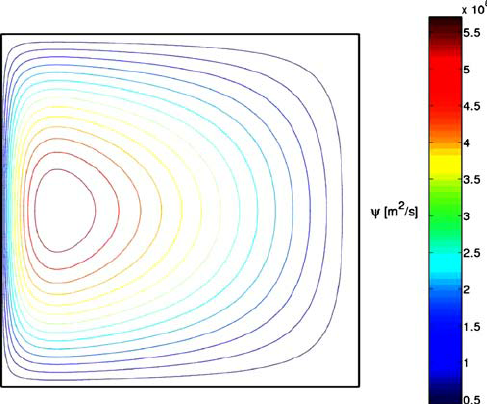
\includegraphics[width=0.4\textwidth]{wbc.png}
	\caption{Streamlines of $\psi$ demonstrating
	western boundary currents.}
\end{figure}

\paragraph{Physical explanation.} The cause of western boundary currents can
be physically explained by vorticity.  The wind stress curl $w < 0$ inputs
negative vorticity in the interior flow. The flow in the western boundary
layer inputs positive vorticity to compensate.

\begin{center}
	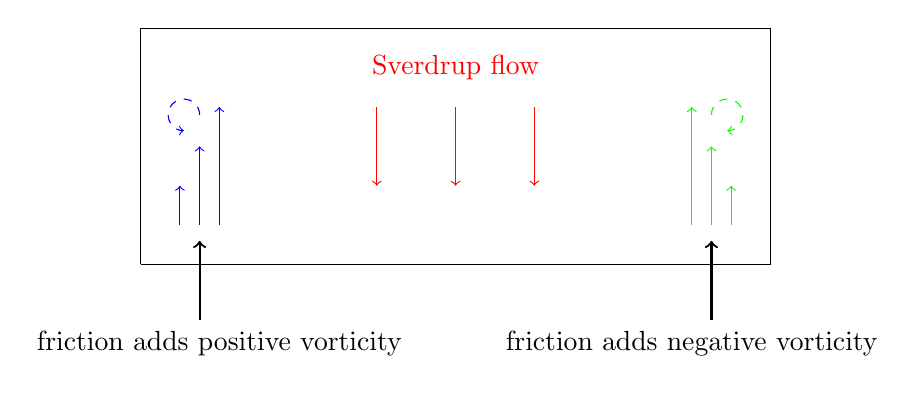
\begin{tikzpicture}
		\draw (0,0) -- (8,0) -- (8,3) -- (0,3) -- (0,0);
		\draw[red,->] (4,2) -- (4,1);
		\draw[red,->] (3,2) -- (3,1);
		\draw[red,->] (5,2) -- (5,1);
		\draw[red] (4, 2.5) node {Sverdrup flow};
		\draw[blue,->] (1,0.5) -- (1,2);
		\draw[blue,->] (0.75,0.5) -- (0.75,1.5);
		\draw[blue,->] (0.5,0.5) -- (0.5,1);
		\draw[blue,dashed,->] (0.75,1.9) arc (0:270:0.2);
		\draw[green,->] (7,0.5) -- (7,2);
		\draw[green,->] (7.25,0.5) -- (7.25,1.5);
		\draw[green,->] (7.5,0.5) -- (7.5,1);
		\draw[green,dashed,->] (7.25,1.9) arc (180:-90:0.2);
		\draw (1, -1) node {friction adds positive vorticity};
		\draw[thick,->] (0.75, -0.7) -- (0.75, 0.3);
		\draw (7, -1) node {friction adds negative vorticity};
		\draw[thick,->] (7.25, -0.7) -- (7.25, 0.3);
	\end{tikzpicture}
\end{center}

\lecture{2/11/20}
\section{Three-dimensional Waves \& Instabilities}
\subsection{Stratification}
\subsubsection{Boussinesq approximation}
We will consider stably stratified flow under the \emph{Boussinesq
approximation}: we assume the density $\rho$ may be split into two parts
$\rho_0$ and $\rho'$ with $\rho_0$ constant and $\rho'/\rho_0 \ll 1$. The
pressure may then also be split into two parts, $p_0(z)$, such that
$-p_0'(z) = \rho_0 g$, and the remainder $p'$. This says $p_0(z)$ is the
hydrostatic pressure and $p'$ is the excess, whilst $\rho_0$ is the density
component in hydrostatic balance, and stratification arises from $\rho'$. The
vertical component of the momentum equations may then be written
\begin{align}
	\frac{\diffD w}{\diffD t} &= -\frac{1}{\rho_0 + \rho'}\frac{\partial
		p_0}{\partial z} - \frac{1}{\rho_0 + \rho'} \frac{\partial
	p'}{\partial z} - g \\
	&= -\frac{1}{\rho_0} \frac{\partial p_0}{\partial z} + \frac{\partial
p_0}{\partial z} \left[ \frac{1}{\rho_0} - \frac{1}{\rho_0 + \rho'}\right] -
\frac{\partial p'}{\partial z} \frac{1}{\rho_0 + \rho'} - g \\
&\approx -\frac{1}{\rho_0} \frac{\partial p'}{\partial z} -
\frac{\rho'}{\rho_0} g
\end{align}
where terms including $\rho'$ are discarded unless multiplying $g$. The
\emph{Boussinesq equations} are therefore
\begin{align}
	\frac{\diffD \symbf{u}}{\diffD t} + \symbf{f} \times \symbf{u} &= -\frac{1}{\rho_0} \nabla
	p' + \frac{\rho'}{\rho_0}\symbf{g} \\
	\nabla \cdot \symbf{u} &= 0 \\
	\frac{\diffD \rho'}{\diffD t} &= 0
\end{align}
where no assumption has been placed on the direction of $\symbf{f}$. 

These equations make clear the role of buoyancy: a light fluid parcel ($\rho'
<0$) experiences an upward force and a heavy fluid parcel ($\rho' > 0$)
experiences a downward force. It is further useful to write $\rho'(x,y,z,t) =
\rho_s (z) + \tilde{\rho}(x,y,z,t)$ where $\rho_s(z)$ is a \emph{background}
or \emph{reference} density and $\tilde{\rho}$ is the \emph{disturbance
density} which is zero for fluid at rest.

The stability of the reference density state is determined by the
\emph{buoyancy frequency} or \emph{Brunt-V\"{a}is\"{a}la frequency} $N$
defined by
\begin{equation}
	N^2 = -\frac{g}{\rho_0} \frac{\diffd \rho_s}{\diffd z}
\end{equation}

\subsubsection{Atmosphere \& ocean stratification}
In the ocean, the buoyancy frequency $N$ is typically $10^{-2} s^{-1}$ in the
upper ocean where stratification is strong, and $5 \times 10^{-4} s^{-1}$ in
the deep ocean, where stratification is weak.

In the atmosphere, calculating $N$ needs to take account of compressibility,
because the density $\rho$ is not conserved by a fluid parcel in reversible,
dissipationless motion. The quantity that is instead conserved is the
\emph{potential temperature}
\begin{equation}
	\theta = T \left(\frac{p}{p_0}\right)^{-2/7}
\end{equation}
where $T$ is temperature. The corresponding buoyancy frequency is
\begin{equation}
	N^2 = -\frac{g}{\theta} \frac{\diffd \theta}{\diffd z}
\end{equation}

In this course we will use the Boussinesq approximation for the atmosphere and
ocean, despite issues with compressibility.

\subsubsection{Internal gravity waves}
We linearise about a resting state with density structure represented by the
buoyancy frequency $N$. For simplicity, background rotation is ignored for the
time being. We define the \emph{buoyancy} $\sigma = -\rho' g/\rho_0$ for
convenience.

\begin{align}
	\tilde{\symbf{u}}_t &= -\frac{1}{\rho_0} \nabla \tilde{p} + \tilde{\sigma}
	\hat{\symbf{z}} \\
	\nabla \cdot \tilde{\symbf{u}} &= 0 \\
	\tilde{\sigma} + N^2 \tilde{w} &= 0
\end{align}

where the notation $\tilde{\symbf{u}}$ denotes the disturbance quantities away from a
state of rest. These can be combined into a single equation for $\tilde{w}$:
\begin{equation}
	\nabla^2 \tilde{w}_{tt} + N^2(\tilde{w}_{xx} + \tilde{w}_{yy}) = 0
\end{equation}

Assuming $N^2$ is constant, seek plane wave solutions $\tilde{w} =
\hat{w}e^{i(kx + ly + mz - \omega t)}$ (real part implicit). This gives a
dispersion relation
\begin{equation}
	\omega^2 = N^2 \frac{k^2 + l^2}{k^2 + l^2 + m^2}
\end{equation}

\begin{itemize}
	\item If $N^2 > 0$ we get oscillatory motion, and if $N^2 < 0$ we get
		exponentially growing disturbances.
	\item We have $0 \le \abs{\omega} \le N$ with the lower limit achieved in
		the limit $k^2 + l^2 \ll m^2$. 
	\item Define $\theta = \tan^{-1}(m(k^2+l^2)^{-1/2})$, so that $\theta$ is
		the angle a surface of constant phase makes with the vertical, so that
		$\omega = \pm N \cos \theta$. Recall
		surfaces of constant phase are perpendicular to $\symbf{k}$. 
	\item Owing to incompressibility $\nabla \cdot \symbf{u} = 0$, $\symbf{k}
		\cdot \hat{\symbf{u}} = 0$ i.e. the velocity vector is perpendicular
		to the wavevector, hence the velocity vector lies in surfaces of constant
		phase. Thus $\theta$ is also the angle that fluid parcel
		trajectories make with the vertical.
	\item Since $\abs{\omega} \le N$, only disturbances with a sufficiently
		low frequency can propagate as waves.  Localised forcing with
		frequency greater than $N$ will remain localised rather than
		propagating. 
	\item In the limit $\theta \to 0$, surfaces of constant phase are vertical
		and the wavevector is horizontal with $\omega \approx \pm N$.
	\item In the limit $\theta \to \frac{\pi}{2}$, surfaces of constant phase
		are horizontal and the wavevector is vertical with $\omega \approx 0$.
	\item Note that the angle of the phase surfaces is independent of wave
		amplitude. Hence waves on a range of spatial scales all have phase
		surfaces oriented in the same direction.
\end{itemize}  

Further, note the group velocity is
\begin{equation}
	\symbf{c}_g \equiv \frac{\partial \omega}{\partial \symbf{k}} = \pm
	\frac{N}{(k^2+l^2)^{1/2} (k^2+l^2+m^2)^{3/2}} (km^2, lm^2, -m(k^2+l^2))
\end{equation}
which gives $\symbf{c}_g \cdot \symbf{k} = 0$, i.e. the group velocity lies in
surfaces of constant phase.

\lecture{4/11/20}
\subsection{3D quasi-geostrophic equations}
\subsubsection{Basic facts about rotation \& stratification}
\begin{enumerate}
	\item Assuming the buoyancy frequency $N$ is constant and $\symbf{f} = f
		\hat{\symbf{z}}$ is vertical, the dispersion relation for small
		amplitude waves is
		\begin{equation}
			\omega^2 = \frac{N^2 k^2 + f^2 m^2}{k^2 + m^2}
		\end{equation}
		where $\symbf{k} = (k,l,m)$. Thus the relative strength of stratification
		vs. rotation is $N/L$ vs. $f/D$, where $L$ is the horizonal
		lengthscale and $D$ is the vertical lengthscale.
	\item Typically, $N \gg f$. In the deep ocean, $N \sim 10^{-3} s^{-1}$ and
		in the upper ocean and atmosphere $N \sim 10^{-2} s^{-1}$, whilst $f
		\sim 10^{-4} s^{-1}$.
	\item Rotation is important only if $L \gg D$, which implies vertical
		velocities are much smaller than horizontal velocities. Hence the
		\emph{hydrostatic approximation} is valid. 
	\item Given $L \gg D$, the Coriolis force may be neglected in the vertical
		momentum equation, and in the horizontal momentum equation only the
		part of the Coriolis force associated with the horizontal velocity is
		important. This can be seen as follows: let $\symbf{f} = \symbf{f}_h +
		\symbf{f}_v$ and $\symbf{u} = \symbf{u}_h + \symbf{u}_v$, where $_h$ and $_v$
		denote horizontal and vertical components respectively. Then,
		\begin{equation}
			\symbf{f} \times \symbf{u} = \symbf{f}_h \times \symbf{u}_h + \symbf{f}_v \times
			\symbf{u}_h + \symbf{f}_h \times \symbf{u}_v + \cancel{\symbf{f}_v \times
			\symbf{u}_v} \approx \symbf{f}_h \times \symbf{u}_h + \symbf{f}_v \times
			\symbf{u}_h
		\end{equation}
		where we have assumed $\abs{\symbf{u}_v} \ll \abs{\symbf{u}_h}$. At low
		latitude, this approximation fails since $\symbf{f}_v \ll \symbf{f}_h$.
		Following the traditional approximation, the horizontal component of the
		Coriolis force is negligible under the hydrostatic approximation
		compared to other terms in the vertical momentum equations.
		Hence only the $\symbf{f}_v \times \symbf{u}_h$ contribution is
		retained in the horizontal momentum equations. This is equivalent to
		replacing $\symbf{f}$ with its vertical component only.
	\item Given the above assumptions, as well as assuming the fluid layer is
		thin compared to the radius of the Earth, we get the \emph{primitive
		equations}. 
\end{enumerate}

Further, we invoke the $\beta$-plane approximation $f = f_0 + \beta y$. The
full $3D$ Boussinesq primitive equations on a $\beta$-plane are
\begin{align}
	\frac{\diffD u}{\diffD t} - (f_0+\beta y)v &= -\frac{1}{\rho_0} p'_x \\
	\frac{\diffD v}{\diffD t} + (f_0 + \beta y) u &= -\frac{1}{\rho_0} p'_y \\
	p'_z &= -\rho' g \\
	\frac{\diffD \rho'}{\diffD t} &= \\
	\nabla \cdot \symbf{u} &= 0
\end{align}

This set of equations is formed of three \emph{prognostic} equations which can
be used to evolve the five dependent variables, and two instantaneous
constraints. There are strong similarities to the shallow water equations on a
$\beta$-plane: at small Rossby number, the shallow water equations have
`fast' modes (e.g. Poincar\'{e} waves \& Kelvin waves for the shallow-water
equations, internal gravity waves for the primitive equations) and `slow'
modes of waves which are close to geostrophic balance.

\subsubsection{Thermal wind equation}
When the Rossby number is small, we expect the flow to be close to geostrophic
balance, so that
\begin{align}
	-fv &= -\frac{1}{\rho_0} p'_x \\
	fu &= -\frac{1}{\rho_0} p'_y
\end{align}
Differentiating with respect to $z$ and using the hydrostatic relation, we
have the \emph{thermal wind equations}
\begin{align}
	fv_z &= -\frac{g}{\rho_0} \rho'_x \\
	fu_z &= \frac{g}{\rho_0} \rho'_y
\end{align}
Here, the density perturbation $\rho'$ can be viewed analogously to
temperature. These equations relate vertical changes in velocity with
horizontal changes in density.

\subsubsection{Potential vorticity}
In the shallow-water equations, the shallow-water potential vorticity was
conserved. Under the Boussinesq primitive equations, instead the
\emph{Rossby-Ertal potential vorticity} $P$ is conserved materially, where
\begin{equation}
	P = \frac{1}{\rho_0} (\symbf{f} +\symbf{\zeta})\cdot \nabla \rho'
\end{equation}
In terms of velocities this is equivalent to
\begin{equation}
	P = \frac{1}{\rho_0} \left[ (f_v + v_x - u_y) \rho'_z + u_z \rho'_y -
		v_z
	\rho'_x\right]
\end{equation}
Note that forcing and dissipation terms are not yet included. These will alter
the material conservation of $P$, giving rise to features in the $P$ field
which can affect or drive the evolution of the flow.

\subsubsection{3D quasi-geostrophic equations}
\paragraph{Primitive equations.} Following the same procedure as with the
shallow-water equations, we aim to find a prognostic equations for the slow
(close to geostrophic balance) motion from the Boussinesq primitive equations
on a $\beta$-plane.

First, we write $\rho'(x,y,z,t) = \rho_s(z) + \tilde{\rho}(x,y,z,t)$ where
$\rho_s(z)$ represents density variation in a hydrostatically balanced state
with no motion, and $\tilde{\rho}$ is associated with motion of the fluid when
it is disturbed from said resting state. We also write $p'(x,y,z,t) = p_s(z) +
\tilde{p}(x,y,z,t)$ where each term is in hydrostatic balance with the
corresponding density term, i.e.
\begin{align}
	\frac{\diffd p_s}{\diffd z} &= -\rho_s g \\
	\frac{\partial \tilde{p}}{\partial z} &= - \tilde{\rho} g
\end{align}
The density equation $\frac{\diffD \rho'}{\diffD t} = 0$ thus becomes
\begin{equation}
	\frac{\diffD \tilde{\rho}}{\diffD t} + w \frac{\diffd \rho_s}{\diffd z} =
	0
\end{equation}

The velocity vield is divided into a part which is in geostrophic balance with
the pressure field (assuming constant Coriolis parameter $f=f_0$) and a remainder, the
\emph{ageostrophic velocity}:
\begin{equation}
	\symbf{u} = \symbf{u}_g + \symbf{u}_a \hspace{2em} \text{where} \,\,\, f_0 \symbf{k}
	\times \symbf{u}_g = -\frac{1}{\rho_0} \nabla_h \tilde{p}
\end{equation}

Note that the vertical component of the geostrophic velocity $\symbf{u}_g$ is
zero, and $\nabla \cdot \symbf{u}_g = 0$. We also assume that the latitudinal
($y$) lengthscale $L_y$ is sufficiently small that $\beta L_y \ll f_0$. Then
if $\Ro \ll 1$, it follows that $\abs{\symbf{u}_a} \ll \abs{\symbf{u}_g}$.
Thus we are domain limited in latitude.

\lecture{6/11/20}
The primitive equations may now be written
\begin{align}
	\left[ \frac{\partial}{\partial t} + (\symbf{u}_g+\symbf{u}_a)\cdot
	\nabla\right] (u_g + u_a) - (f_0+\beta y) (v_g + v_a) &=
	-\frac{1}{\rho_0} \frac{\partial \tilde{p}}{\partial x} \label{eq:prim1}\\
	\left[ \frac{\partial}{\partial t} + (\symbf{u}_g+\symbf{u}_a)\cdot
	\nabla\right] (v_g + v_a) + (f_0+\beta y) (u_g + u_a)&=
	-\frac{1}{\rho_0} \frac{\partial \tilde{p}}{\partial y}\label{eq:prim2} \\
	-\frac{\partial \tilde{p}}{\partial z} - \tilde{\rho} g &= 0 \\
	\left[\frac{\partial}{\partial t} + (\symbf{u}_g+\symbf{u}_a)\cdot
	\nabla\right] \tilde{\rho} + w_a \frac{\diffd \rho_s}{\diffd z} &= 0 \\
	\frac{\partial u_a}{\partial x} + \frac{\partial v_a}{\partial y} +
	\frac{\partial w_a}{\partial z} &= 0
\end{align}

\paragraph{Approximation validity.}
\begin{itemize}
	\item Given that $\Ro \ll 1$ we may approximate $\frac{\diffD
		\symbf{u}}{\diffD t}$ by $\frac{\diffD_g \symbf{u}_g}{\diffD t}$ where
		$\frac{\diffD_g}{\diffD t} = \partial_t + \symbf{u}_g \cdot \nabla$
	\item Also $\beta y \symbf{u}$ can be approximated by $\beta y
		\symbf{u}_g$. 
	\item Note that $f_0(u_a, v_a)$ and $\beta y(u_g, v_g)$ are of similar size. Hence
the requirement $\beta L_y / f_0 \ll 1$ is better expressed by $\beta L_y/f_0
\sim \Ro$. 
	\item Also, $w_a \frac{\diffd \rho_s}{\diffd z}$ is retained, but $w_a
		\frac{\diffd \tilde{\rho}}{\diffd z}$ is not, which requires
		$\abs{\diffd \tilde{\rho}/\diffd z} \ll \abs{\diffd \rho_s / \diffd
		z}$. Denoting the horizontal scale as $L$ and the vertical scale as
		$D$, the thermal wind equation gives $g \tilde{\rho}/L \rho_0 \sim f_0
		U/D$ where $U$ is the typical horizontal velocity scale. Hence we have
		\begin{equation} 
			\frac{\tilde{\rho}_z}{\rho_{s,z}} \sim \frac{f_0 U L
			\rho_0}{gD^2 \rho_{s,z}} = \frac{U}{f_0 L} \left( \frac{L f_0}{N
			D}\right)^2 = \Ro \Bu 
		\end{equation} where $\Bu \equiv (L f_0 / D
		N)^2$ is the \emph{Burger number} and we have used $\frac{N^2 D}{g}
		\sim \rho_s / \rho_0$ which follows from the definition of $N$. For
		our approximation to be valid, we require $\Ro \Bu \ll 1$. If $\Bu
		\sim 1$, then this is implied by $\Ro \ll 1$.  
\end{itemize}

\paragraph{Quasi-geostrophic potential vorticity.} 
To reduce the primitive equations to a single
prognostic equation, we eliminate $\symbf{u}_a$ by taking the curl of horizontal
momentum, i.e. $\partial_x \eqref{eq:prim2} - \partial_y \eqref{eq:prim1}$.
The non-divergence of geostrophic velocity then gives a vorticity equation
\begin{equation}
	\frac{\diffD_g}{\diffD t} \left[ \frac{\partial v_g}{\partial x} -
		\frac{\partial u_g}{\partial y} \right] + \beta v_g + f_0 \left[
		\frac{\partial u_a}{\partial x} + \frac{\partial v_a}{\partial y}
	\right] = 0
\end{equation}
Finally, we eliminate $u_a, v_a$ and $w_a$ using the remaining primitive
equations to give
\begin{equation}
	\frac{\diffD_g}{\diffD t} \left[ \frac{\partial v_g}{\partial x} -
		\frac{\partial u_g}{\partial y} \right] + \beta v_g +
		f_0\frac{\partial}{\partial z} \left[ \frac{\diffD_g
		\tilde{\rho}}{\diffD t} / \frac{\diffd \rho_s}{\diffd z}\right] = 0
\end{equation}

We now define a streamfunction $\psi = \frac{\tilde{p}}{\rho_0 f_0}$ analogous
to the geostrophic streamfunction. Then $u = -\psi_y, v = \psi_x$ from
hydrostatic balance $\tilde{\rho} = - \rho_0 f_0 \psi_z / g$. Our prognostic
equation, called the \emph{quasi-geostrophic potential vorticity equation} is
then
\begin{equation}
	\frac{\diffD_g}{\diffD t} \left[ \psi_{xx} + \psi_{yy} + \left(\frac{f_0^2
	\psi_z}{N^2}\right)_z \right] + \beta \psi_x = 0\label{eq:qgpv}
\end{equation}
or equivalently $\frac{\diffD_g q}{\diffD t} = 0$ where $q$ is the
quasi-geostrophic potential vorticity
\begin{equation}
	q = \psi_{xx} + \psi_{yy} + \left( \frac{f_0^2 \psi_z}{N^2}\right)_z +
	\beta y
\end{equation}
and $N^2 = -\frac{g}{\rho_0} \frac{\diffd \rho_s}{\diffd z}$. In terms of the
QGPV, the (geostrophic) material derivative is
\begin{equation}
	\frac{\diffD_g}{\diffD t} = \frac{\partial}{\partial y} - \psi_y
	\frac{\partial}{\partial y} + \psi_x \frac{\partial}{\partial y}
\end{equation}
Under the quasi-geostrophic approximation, $q$ is conserved following the
horizontal geostrophic flow. The QGPV equation is an approximation to the
statemenet of material conservation of Rossby-Ertel potential vorticity
following the flow along $\rho'$ surfaces in a Boussinesq flow, or $\theta$
surfaces in a compressible flow.

If $q$ is known, then $\psi$ can be calculated via the \emph{potential
vorticity inversion operator}
\begin{equation}
	\psi = \left[\partial_x^2 + \partial_y^2 + \partial_z
	\left(\frac{f_0^2}{N^2} \partial_z\right)\right]^{-1} (q-\beta y)
\end{equation}
Application of this operator requires boundary conditions on $\psi$ or its
derivatives.

\paragraph{Boundary conditions.}
\begin{itemize}
	\item At rigid side boundaries, we require the normal component of $\symbf{u}$ is
		zero (no flux condition), which requires $\psi$ constant along the
		boundary.
	\item At rigid top or bottom boundaries, we require the kinematic boundary
		condition to be satisfied, i.e. $\frac{\diffD z}{\diffD t} = w =
		\frac{\diffD h}{\diffD t}$ on the boundary $z = z_b +h$ where $z_b$ is
		constant and $h$ is the topographic perturbation. We may express $w_a$
		in terms of other variables via the density equation to get
		\begin{equation}
			w \sim w_a = -\frac{\diffD_g \tilde{\rho}}{\diffD t}
			\left(\frac{\diffd \rho_s}{\diffd z}\right)^{-1} = \frac{\diffD
			h}{\diffD t} \approx \frac{\diffD_g h}{\diffD t}
		\end{equation}
		Hence $h \sim \tilde{\rho}\left(\frac{\diffd \rho_s}{\diffd
		z}\right)^{-1} \sim D \left( \frac{U}{f_0 L}\right) \left(\frac{L^2
		f_0^2}{N^2 D^2}\right) = \Ro \Bu D$, so we require $h \ll D$. The
		boundary condition may then be linearised, so that it can be applied
		at $z = z_b$.  Writing $\tilde{\rho}$ in terms of $\psi$, we have
		\begin{equation} 
			\frac{\diffD_g}{\diffD t} \psi_z = -\frac{N^2}{f_0}
			\frac{\diffD_g}{\diffD t} h 
		\end{equation} 
		at $z = z_b$. This is a prognostic equation for $\psi_z$ at the bottom
		surface which relates (physically) to material rate of change of
		density or temperature.
\end{itemize}

\paragraph{Physical interpretation of QGPV.} 
The density or temperature at horizontal boundaries have similar importance to
the QGPV in the interior of the flow. The physical interpretations of different
contributions to the quasi-geostrophic potential vorticity $q$ are
\begin{align}
	q \,\,\,= \hspace{3em}&\hspace{1em}\psi_{xx} + \psi_{yy} \hspace{3em}+ &&\left( \frac{f_0^2}{N^2} \psi_z
	\right)_z \hspace{3em}+ && \hspace{1em}\beta y \\
	&\text{relative vorticity} && \text{stretching} && \text{planetary
vorticity}	
\end{align}
The stretching measures vertical gradients in density perturbations, i.e. the
amount by which nearby density surfaces move apart or together. The ratio of
the relativity vorticity term to the stretching term is $1/\Bu$. If $\Bu \ll
1$ then relative vorticity dominates, whilst if $\Bu \gg 1$ then stretching
dominates. If $\Bu \sim 1$ the terms are comparable and the ratio of
horizontal to vertical scales $L/D \sim N /f_0$ is implied by this condition
as is called \emph{Prandtl's ratio of scales}.

The 3D quasi-geostrophic equations have a structural similarity to the
equations of 2D vortex dynamics, in that there is a non-local dependence of
$\psi$ on $q$. In 2D vortex dynamics, the non-locality is purely horizontal,
whilst in the 3D quasi-geostrophic equations the non-locality is also in the
vertical and the PV field in a localised region at a given level influences
the $\psi$ field outside that region on the same level \emph{and} at other
levels.

If $N$ is constant in height, then the PV operator is isotropic in scales
coordinates $x, y, Nz/f_0$. The evolution equations are not isotropic since
the flow only has horizontal components. Therefore we expect solutions of the
QG equations to tend towards isotropy in the coordinates above, but the
isotropy is likely not exact.

\lecture{3/11/20}
\subsubsection{Quasi-geostrophic `point vortex'}
Here we will consider an illustrative simple 3D quasi-geostrophic flow
calculation known as a `point vortex', i.e. we assume
\begin{equation}
	q = U L^2 \delta(x,y, Nz/f_0)
\end{equation}
where $\delta(\x)$ is the Dirac delta function and solve
\begin{equation}
	\psi_{xx} + \psi_{yy} + \left[ \frac{f_0^2}{N^2} \psi_z\right]_z = UL^2
	\delta(x,y,z)
\end{equation}
for $\psi(x,y,z)$. We assume that $N$ is constant and that the $\beta y$ term
in QGPV can be neglected. $U$ and $L$ are respectively a constant velocity and
a constant length, to give dimensional consistency. First, rescale $z$ by
defining $\bar{z} = Nz/f_0$. In Cartesians $(x,y,\bar{z})$, we now have a 3D
Laplacian and we deduce the solution with $\psi \to 0$ as $\abs{x}, \abs{y},
\abs{\bar{z}}$ tend to infinity is
\begin{equation}
	\psi(x,y,z) = -\frac{UL^2}{4\pi} \frac{1}{\sqrt{x^2+y^2+\bar{z}^2}} =
	-\frac{1}{4\pi} \frac{1}{(x^2+y^2+N^2z^2/f_0^2)^{1/2}}
\end{equation}
The horizontal velocity components are then
\begin{equation}
	(u,v) = \frac{UL^2}{4\pi} \frac{(-y,x)}{(x^2+y^2+N^2z^2/f_0)^{3/2}}
\end{equation}
and the density perturbation is given by
\begin{equation}
	\tilde{\rho} = -\frac{f \rho_0}{g} \psi_z = -\frac{f \rho_0 U L^2}{4\pi g}
	\frac{z}{(x^2+y^2+N^2z^2/f_0^2)^{3/2}}
\end{equation}
Far from the point vortex, the sum of the relative vorticity and the
stretching term in $q$ is zero, but, consistent with the fact the circulation
(both velocity and density perturbations) extend away from the point vortex,
they are individually non-zero.

\subsection{Waves \& instabilities in 3D QG}
\subsubsection{Framework}
Consider the quasi-geostrophic potential vorticity equation \eqref{eq:qgpv} as
a starting point and consider small-amplitude disturbances to a background
(geostrophic) flow which satisfies these equations. The background flow is
assumed to be only in the $x$-direction and to depend only on $y$, i.e.
\begin{equation}
	(u_g,v_g) = (U(y,z), 0)
\end{equation}
There is a corresponding background quasi-geostrophic stream function
$\Psi(y,z)$ such that $U = -\Psi_y$ and a background quasi-geostrophic
potential vorticity $Q(y,z) = \Psi_{yy} + (f_0\Psi_z/N^2)_z + \beta y$.

As opposed to deriving the Boussinesq approximation, we will now use the prime
$()'$ notation to denote disturbance quantities. The quasi-geostrophic
equations retaining only linear terms in disturbance quantities are
\begin{equation}
	\left[ \frac{\partial}{\partial t} + U(y,z) \frac{\partial}{\partial
	x}\right](\psi'_{xx} + \psi'_{yy} + (\frac{f_0^2}{N^2} \psi'_z)_z) +
	(\beta - U_{yy} - (\frac{f_0^2}{N^2} U_z)_z)\psi'_x = 0 \label{eq:QGPVlin}
\end{equation}
The boundary condition at any boundary for top and bottom is here  illustrated
for $z=0$,
\begin{equation}
	\left[\frac{\partial}{\partial t} + U(y,0) \frac{\partial}{\partial
		x}\right] \psi'_z - U_z(y,0) \psi'_x = -\frac{N^2}{f_0} \left[
			\frac{\partial}{\partial t} + U(y,0) \frac{\partial}{\partial x}
		\right] h'
\end{equation}

\begin{itemize}
	\item The quantity $\beta - U_{yy} - (f_0^2 U_z / N^2)_z$ plays a
		potentially important role: this is the $y$-gradient of QGPV in the
		background state.
	\item The quantity $U_z(y,0)$ in the boundary condition, which is
		proportional to the $y$-gradient of density at $z=0$ may also be
		important.
	\item Note that the boundary condition is derived from the density
		equation $\frac{\diffD \rho'}{\diffD t} = 0$, and the density
		distribution at the boundary has similar status in the equtions to the
		interior distribution of QGPV.
\end{itemize}

\subsubsection{Rossby waves -- vertical modes}
Consider the $3D$ quasi-geostrophic equations in an oceanic configuration with
a free surface at $z=0$ in the resting undisturbed state, and a flat bottom at
$z = -H$ with buoyancy frequency $N(z)$ which is not assumed constant. Assume
that in the undisturbed state the height of the free surface is
\begin{equation}
	z = \eta'(x,y,t)
\end{equation}
and assume disturbances are suitably small that we may estimate $p(x,y,0,t) =
p_{\text{atm}} + \rho_0 g \eta'$. Then at $z=0$ we have $\rho_0 g w =
\frac{\diffD_g \tilde{p}(z=0)}{\diffD t}$. Using the expression for pressure
and vertical velocity under the quasi-geostrophic approximation, the boundary
condition at $z=0$ is
\begin{equation}
	\frac{\diffD_g \psi'_z}{\diffD t} + \frac{N^2}{g} \frac{\diffD_g
	\psi'}{\diffD t} = 0
\end{equation}
Similarly, at $z=-H$ the boundary condition is
\begin{equation}
	\frac{\diffD_g \psi'_z}{\diffD t} = 0 
\end{equation}

The QGPV equation then reduces to
\begin{equation}
	\left( \psi'_{xx} + \psi'_{yy} + (\frac{f_0^2}{N^2}
	\psi'_z)_z\right)_t + \beta \psi'_x = 0
\end{equation}

Seek solutions of the form $\psi'(x,y,z,t) = \phi(x,y,t) P(z)$ where $P$
satisfies
\begin{equation}
	\frac{\diffd}{\diffd z} \left[ \frac{1}{N^2} \frac{\diffd P}{\diffd
	z}\right] = -\frac{1}{gh} P
\end{equation}
for consistency, where $h$ is a suitably constant and at $z=0$ $P$ satisfies
$P_z + (N^2/g)P = 0$ and at $z=-H$ $P$ satisfies $P_z = 0$. This is an
eigenvalue for $h$, called the \emph{vertical structure equation}, and we
expect a countable sequence of possible values $h_1 > h_2 > \dots > 0$, with
the maximum value $h_1$ corresponding to the simplest possible structure for
$P(z)$.

\begin{itemize}
	\item The height $g/N^2$ is typically large compared to the depth $H$ (or
		the vertical length scale associated with variations in
		stratification). Thus the boundary condition at $z=0$ can be
		approximated by $P_z = 0$. This is the \emph{rigid lid approximation},
		equivalent to imposing zero vertical velocity. 
	\item Using the rigid lid approximation, the boundary condition gives $P$
		non-zero at $z=0$ and the solution may therefore be used to give a
		good first estimate of the pressure variation at $z=0$ and hence the
		variation in free-surface height.
	\item If $N = N_0$ constant then the largest value $h_1 = N_0^2
		H^2/g\pi^2$, i.e.
		\begin{equation}
			(gh_1)^{1/2} = N_0 H/\pi
		\end{equation}
		In this case, $P_1(z)$ has a single zero in the interior layer. The
		vertical displacement corresponds to $P_1'(z)$ which has a single
		maximum in the interior of the layer. This is the \emph{first
			baroclinic mode}\footnote{Baroclinic means `with vertical
			structure', where $P$ is not simply related to $\rho$, whereas
		barotropic means $p$ is a function of $\rho$ at all levels.}. For
		realistic ocean stratification, we typically find $(gh_1)^{1/2}
		\approx 3 ms^{-1}$ and the second baroclinic mode $(gh_2)^{1/2}
		\approx 1 ms^{-1}$.
		\begin{center}
			\begin{tikzpicture}[scale=3];
				\draw[thick,->] (-1,0) -- (1,0) node[below,right] {$\rho(z)$};
				\draw[thick,->] (0,0) -- (0,1.2) node[left]{$z$};
				\draw[smooth,blue] plot[domain=0:1,variable=\y]
				({1/(1+exp(-10*(\y-0.5)))-0.5},{\y});
				\draw[dashed] (-1,1) -- (1, 1) node [right,below] {$z=0$};
				\draw (-0.5, -0.1) node {$z=-H$};
			\end{tikzpicture}
		\end{center}
	\item Given $h_i$ and $P_i(z)$ the corresponding equation for
		$\phi_i(x,y,t)$, describing the horizontal structure of the
		$i$\textsuperscript{th} mode is
		\begin{equation}
			\left( \phi_{ixx} + \phi_{iyy} - \frac{f_0^2}{gh_i}
			\phi_i\right)_t + \beta \phi_{ix} = 0
		\end{equation}
		which is the quasi-geostrophic equation for shallow water of depth
		$h_i$. 
	\item We have reduced the three-dimensional problem to an equivalent set
		of single layer problem, one for each mode, with the layer depths
		determined as eigenvalues of the vertical structure equation.
	\item For each vertical mode there is a corresponding Rossby radius of
		deformation given by
		\begin{equation}
			L_{iR} = \frac{(gh_i){1/2}}{f_0}
		\end{equation}
		THe first baroclinic mode has $L_{1R} \approx 30 km$, and the second
		$L_{2R} \approx 10 km$ at mid-latitutes.
	\item For scales much greater than $L_{R}$ the single-layer dispersion
		relation implies that the phase and group velocities are westward and
		given by $\beta L_R^2$. The waves are non-dispersive in this limit.
		For the first baroclinic mode, this gives a Rossby wave speed of
		approximately $1.5 \times 10^{-2} ms^{-1}$ which is extremely small,
		and makes observation difficult.
	\item The wave speed increases towards the equator, but the formula breaks
		as the equator is approached and we must instead consider equatorial
		Rossby waves (later in course).
\end{itemize}

\lecture{11/11/20}
\subsubsection{Baroclinic instability}
Here we consider a flow for which disturbances that are small-amplitude
initially may grow substantially in ampltiude.  In the atmosphere and ocean,
an important instability mechanism is associated with sloping density
surfaces, i.e. horizontal density gradients, present due to vertical shear.
Here we consider a problem due to Eady. Consider a basic state on an
$f$-plane, with constant buoyancy frequency $N$ and flow in the $x$-direction
$U = \Lambda z$, so that $\psi_0 = -\Lambda z y$, $\Lambda > 0$. We use the
rigid lid approximation with horizontal rigid boundaries at $z=0$ and $z= H$.

The $y$-gradient of the QGPV is
\begin{equation}
	\beta - U_yy - (\frac{f_0^2}{N^2} U_z)_z = -(\frac{f_0^2}{N^2} \Lambda)_z
	= 0
\end{equation}
Hence the linearised QGPV equation reduces to
\begin{equation}
	q'_t + \Lambda z q'_x = 0
\end{equation}
where $q'(x,y,z,t) = q'(x-\Lambda z t, y, z, 0)$. Physically, this says the
$q'$ field at any level is advected by the horizontal flow. Thus the $q'$
field is of no consequence in the analysis of possible instability and we
choose $q'(x,y,z,0)= 0$ for convenience. The boundary conditions are
\begin{align}
	\psi'_{zt} - \Lambda \psi'_x &= 0 &&\text{at}\,\,\, z=0 \\
	\psi'_{zt}+\Lambda H \psi'_{zx} - \Lambda \psi'_x &= 0 &&\text{at} \,\,\,z
	=H
\end{align}
and the interior flow satisfies
\begin{equation}
	\psi'_{xx} + \psi'_{yy} + \frac{f_0^2}{N^2} \psi'_{zz} = 0
\end{equation}

Seek plane wave solutions of the form
\begin{equation}
	\psi' = \Re\left[ \hat{\psi}(z) e^{i(kx + ly - kct)}\right]
\end{equation}
with this form, $c$ is the complex phase speed in the $x$-direction. There
will be an instability if $k \Im\left[c\right] > 0$. Note wlog we can take $k
> 0$. Substituting into the interior equation we find 
\begin{align}
	\hat{\psi}_{zz} - \mu^2 \hat{\psi} &= 0\\
	\mu &= \frac{N_0}{f_0} (l^2+k^2)^{1/2} \\
	\implies \hat{\psi} &= A e^{\mu z} + Be^{-\mu z}
\end{align}

Substituting into the boundary conditions and solving for $c$ we find
\begin{equation}
	c = \frac{1}{2} \Lambda H \left[ 1 \pm \sqrt{F(\mu H)}\right]
\end{equation}
where
\begin{equation}
	F(\mu H) = 1-4\frac{\coth \mu H}{\mu H} + \frac{4}{\mu^2 H^2}
\end{equation}

It can be shown that $F$ is an increasing function with $F(\mu H) \to 1$ as
$\mu H \to \infty$. Hence there is an instability if $\mu H < \hat{\mu}_c =
0.2399$ where $F(\hat{\mu}_c) = 0$. The growth rate is given by
\begin{equation}
	k\Im\left[c\right] = \frac{f_0 \Lambda}{N} \frac{k}{(k^2+l^2)^{1/2}}\left[
	\frac{1}{2}\mu H \sqrt{-F(\mu H)}\right]
\end{equation}

\paragraph{Comments.}
\begin{itemize}
	\item The formula for the growth rate shows that for given $\mu$ the
		growth rate is maximised when $l$ is zero. Hence the maximum growth
		rate will occur when $\frac{1}{2}\mu H \sqrt{-F(\mu H)}$ is maximised
		over $\mu$, and for this value of $\mu$, when $l = 0$. The maximum
		value is in fact $0.31$ when $\mu H = 1.61$.
	\item Hence the maximum growth rate in the Eady problem is $0.31 \frac{f_0
		\Lambda}{N}$, i.e. proportional to the vertical shear $\Lambda$. In
		this case, the $x$-wavenumber $k$ is $1.61 f_0/NH$ and $l = 0$.
	\item In the limit $\mu H \to \infty$, $c/\Lambda H \to 1/\mu H$ or
		$c/\Lambda H \to 1 - 1/\Mu H$. In the first case, $B \gg A$ and the
		wave is \emph{bottom trapped}. In the second case $A \sim B$ and since
		$\mu H \gg 1$, the wave is \emph{top trapped}. The top wave propagates
		in the negative $x$-direction (against the flow) and the bottom wave
		propagates with the flow.
	\item If there is only a lower boundary, we find dispersion relation $c =
		\Lambda/\mu$ hence we have an eastward travelling wave trapped at the
		lower boundary (for positive vertical shear). 
	\item The propagation mechanism may be understood in terms of circulation
		induced by a surface density change. Anomalies in the boundary density
		influence the interior $\psi$, which generates a flow which supports
		the anomalies.
	\item In the case of two boundaries, the instability mechanism results
		from the phase locking of the trapped top and bottom waves. The fact
		the instability occurs only for sufficiently small $\mu H$ is because
		at larger $\mu H$ the interaction between the boundary waves is too
		weak.
	\item If there were instead side boundaries at $y = 0$ and $y = L$ then $l
		= \pm n \pi /L$ would be quantised with $n = 1, 2, \dots$. 
\end{itemize}

\paragraph{Density transport.}
Consider the density transport by the growing wave. The density flux in the
$y$-direction is $\bar{\rho' v'}$ where the bar represents an $x$-average. In
terms of the QG streamfunction, we have
\begin{align}
	\bar{\rho' v'} &= - \frac{\rho_0 f_0}{g}\bar{\psi'_x \psi'_z}\\
	&= \dots\\
	&= \frac{2k\mu^2}{f_0} \frac{\diffd \rho_s}{\diffd z} \frac{\abs{A}^2
\Lambda \Im\left[c\right]}{\abs{c^*\mu -\Lambda}^2} < 0
\end{align}
Hence the density flux is negative, i.e. light fluid is transported in the
positive $y$-direction and heavy fluid in the negative $y$-direction, tending
to weaken the $y$-gradient of density and hence release some of the potential
energy of the background state.

Thus a growing disturbance on a basic state with a positive density gradient
equtor to pole produces a poleward flux of light fluid, and an equatorward
flux of heavy fluid. This is a \emph{baroclinic instability}. 

\lecture{13/11/20}
\subsection{Fronts}
A \emph{front} is an elongated region with a large horizontal density
gradient. These are associated with
\begin{itemize}
	\item large vertical motion
	\item severe weather
	\item exchange of water between ocean surface and interior
\end{itemize}

The process by which fronts develop is called \emph{frontogenesis}.

\subsubsection{Frontogenesis function}
Consider the QG buoyancy equation with $\abs{\symbf{u}_a} \ll
\abs{\symbf{u}_g}$ and $b \equiv = -\frac{g\rho}{\rho_0}$.
\begin{equation}
	\frac{\partial b}{\partial t} + \symbf{u}_g \cdot \nabla_H b + w_a N^2 = 0
	\label{eq:qgbuoyancy}
\end{equation}
Using index notation, $\nabla_H \eqref{eq:qgbuoyancy}$ gives
\begin{equation}
	\partial_t \partial_i b + (\partial_i u_{g,j})(\partial_j b) +
	u_{g,j}\partial j \partial i b + N^2 \partial_i w_a = 0
\end{equation}
The buoyancy equation is supplemented by boundary conditions $w_a = 0$ at
$z=0, H$. At these boundaries, we therefore have
\begin{equation}
	\frac{\diffD_g}{\diffD t} \nabla_H b = \symbf{Q}
\end{equation}
where $\frac{\diffD_g}{\diffD t} = \partial_t + \symbf{u}_g \cdot \nabla_H$ as
usual and the \emph{Q-vector} is
\begin{equation}
	\symbf{Q} \equiv (-u_{g,x} b_x - g_{g,x} b_y, -u_{g,y} b_x - v_{g,y}b_y)
\end{equation}
The gradient of the equation applicable at the boundaries $z=0,H$ is then
\begin{equation}
	\frac{\diffD_g}{\diffD t} \abs{\nabla_H b}^2 = 2\symbf{Q}\cdot\nabla_H b
	\label{eq:frontogenesis}
\end{equation}
where the right hand side is the \emph{frontogenesis function}. This equation
says that the gradients in buoyancy are advected by $\symbf{Q}$.

\subsubsection{Vertical velocity in 3D QG equations}
Recall the 3D quasi-geostrophic equations can be written
\begin{align}
	\frac{\diffD_g}{\diffD t} \symbf{u}_g + f \hat{\symbf{z}}\times
	\symbf{u}_g &= 0 \label{eq:3dqg.1} \\
	\frac{\diffD_g}{\diffD t} b + w_a N^2 &= 0 \label{eq:3dqg.2} \\
	\nabla_H \cdot \symbf{u}_g = 0 \label{eq:3dqg.3} \\
	\nabla_H \cdot \symbf{u}_a + w_{a,z} &= 0 \label{eq:3dqg.4}
\end{align}

Recall also the thermal wind equations relating horizontal velocity gradients
and buoyancy gradients
\begin{equation}
	fu_{g,z} = -b_y, \hspace{2em} fv_{g,z} = b_x
\end{equation}

Our aim is to eliminate the geostrophic velocities to give a diagnostic
equation relating the Q-vector and the vertical ageostrophic velocity. Using
thermal wind balance and the $x$ component of $\partial_z \eqref{eq:3dqg.1}$
we have
\begin{equation}
	-\frac{\diffD_g}{\diffD t} b_y - b_y u_{g,x} + b_x u_{g,y} - f^2 v_{a,z} =
	0 \label{eq:front1}
\end{equation}
We form a similar equation via $\partial_y \eqref{eq:3dqg.2}$:
\begin{equation}
	\frac{\diffD_g}{\diffD t} b_y + u_{g,y} b_x + v_{g,y} b_y + w_{a,y}N^2 = 0
	\label{eq:front2}
\end{equation}
Now combining \eqref{eq:front1} and \eqref{eq:front2} and from continuity,
$v_{g,y} = -u_{g,x}$, gives
\begin{equation}
	N^2 w_{a,y} - f^2 v_{a,z} = -2u_{g,y} b_x - 2U_{g,x} b_y \label{eq:front3}
\end{equation}

Applying the same process with the $y$ component of $\partial_z
\eqref{eq:3dqg.1}$ gives
\begin{equation}
	N^2 w_{a,x} - f^2 u_{a,z} = -2v_{g,y} b_x - 2v_{g,x} b_y \label{eq:front4}
\end{equation}

Finally we eliminate $\symbf{u}_g$ in favour of $\symbf{Q}$ via $\partial_x
\eqref{eq:front4} + \partial_y \eqref{eq:front3}$ and using \eqref{eq:3dqg.4}
to give the \emph{QG Omega equation}.
\begin{equation}
	N^2 \nabla_H^2 w_a + f^2 w_{a,zz} = 2 \nabla_H \cdot \symbf{Q}
\end{equation}
This is a diagnostic elliptic equation, which can be solved subject to
boundary conditions on $w$. Note that we have eliminated any time derivatives
in this equation, making it diagnostic.

\lecture{16/11/20}
\subsubsection{Ageostrophic secondary circulation (ASC)}
Consider a front $\frac{\partial b}{\partial x} > 0$ in thermal wind balance
\begin{equation}
	\frac{\partial \symbf{u}_g}{\partial z} = \inv{f}\frac{\partial
	b}{\partial x}\hat{\symbf{y}}
\end{equation}
subject to horizontal strain $\symbf{u}_g$ such that
\begin{equation}
	\frac{\partial u_g}{\partial x} = -\frac{\partial v_g}{\partial y} =
	-\alpha
\end{equation}
with $\alpha > 0$ constant. Note that to be fully clear, the velocity should
be written $\symbf{u} = \symbf{u}_g + \symbf{u}_s$ where $\symbf{u}_g$ is the
thermal wind and $\symbf{u}_s$ is the straining velocity. The Q-vector is then $\symbf{Q} = (\alpha b_x, 0)$
so that $\symbf{Q} \cdot \nabla b > 0$ for $\alpha > 0$. The influence of this
front is as follows. Note that each of these influences happen simultaneously,
but for clarity we consider the consequences one by one. Our initial set-up is
shown below with red lines representing buoyancy surfaces.\\
\begin{center}
\hspace{.35in}
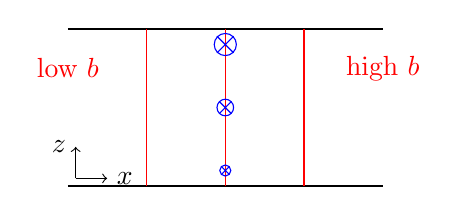
\begin{tikzpicture}		
	\draw[thick] (-2,0) -- (2,0);
	\draw[thick] (-2,2) -- (2,2);
	\draw[->] (-1.9, 0.1) -- (-1.5, 0.1) node[right] {$x$};
	\draw[->] (-1.9, 0.1) -- (-1.9, 0.5) node[left] {$z$};
	\draw[red] (0,0) -- (0,2);
	\draw[red] (1,0) -- (1,2);
	\draw[red] (-1,0) -- (-1,2);
	\draw[red] (-2, 1.5) node {low $b$};
	\draw[red] (2, 1.5) node {high $b$};
	\draw[blue] (0,1.8) node[cross=3.4pt,blue] {};
	\draw[blue] (0,1.8) circle (4pt);
	\draw[blue] (0,1) node[cross=2.6pt,blue] {};
	\draw[blue] (0,1) circle (3pt);
	\draw[blue] (0,0.2) node[cross=1.8pt,blue] {};
	\draw[blue] (0,0.2) circle (2pt);
\end{tikzpicture}
\end{center}

\begin{enumerate}
	\item A convergent strain $\alpha > 0$ increases $\frac{\partial
		b}{\partial x}$, by \eqref{eq:frontogenesis}.
		\begin{center}
			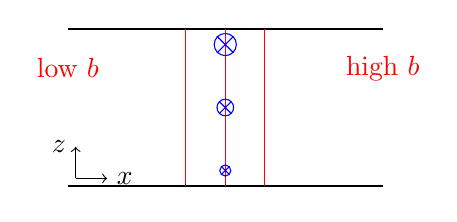
\begin{tikzpicture}		
				\draw[thick] (-2,0) -- (2,0);
				\draw[thick] (-2,2) -- (2,2);
				\draw[->] (-1.9, 0.1) -- (-1.5, 0.1) node[right] {$x$};
				\draw[->] (-1.9, 0.1) -- (-1.9, 0.5) node[left] {$z$};
				\draw[red] (0,0) -- (0,2);
				\draw[red] (0.5,0) -- (0.5,2);
				\draw[red] (-0.5,0) -- (-0.5,2);
				\draw[red] (-2, 1.5) node {low $b$};
				\draw[red] (2, 1.5) node {high $b$};
				\draw[blue] (0,1.8) node[cross=3.4pt,blue] {};
				\draw[blue] (0,1.8) circle (4pt);
				\draw[blue] (0,1) node[cross=2.6pt,blue] {};
				\draw[blue] (0,1) circle (3pt);
				\draw[blue] (0,0.2) node[cross=1.8pt,blue] {};
				\draw[blue] (0,0.2) circle (2pt);
			\end{tikzpicture}
		\end{center}
	\item The increase in $\frac{\partial b}{\partial x}$ results in an
		increase in the hydrostatic pressure gradient in the $x$-direction.
		The unbalanced pressure gradient drives an \emph{ageostrophic
		secondary circulation} $\symbf{u}_a$.
		\begin{center}
			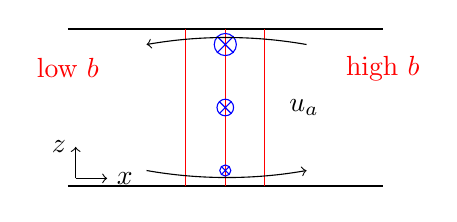
\begin{tikzpicture}		
				\draw[thick] (-2,0) -- (2,0);
				\draw[thick] (-2,2) -- (2,2);
				\draw[->] (-1.9, 0.1) -- (-1.5, 0.1) node[right] {$x$};
				\draw[->] (-1.9, 0.1) -- (-1.9, 0.5) node[left] {$z$};
				\draw[red] (0,0) -- (0,2);
				\draw[red] (0.5,0) -- (0.5,2);
				\draw[red] (-0.5,0) -- (-0.5,2);
				\draw[red] (-2, 1.5) node {low $b$};
				\draw[red] (2, 1.5) node {high $b$};
				\draw[blue] (0,1.8) node[cross=3.4pt,blue] {};
				\draw[blue] (0,1.8) circle (4pt);
				\draw[blue] (0,1) node[cross=2.6pt,blue] {};
				\draw[blue] (0,1) circle (3pt);
				\draw[blue] (0,0.2) node[cross=1.8pt,blue] {};
				\draw[blue] (0,0.2) circle (2pt);
				\draw[->] (-1,0.2) arc (-100:-80:5.85);
				\draw[<-] (-1,1.8) arc (100:80:5.85);
				\draw (1, 1) node {$\symbf{u}_a$};
			\end{tikzpicture}
		\end{center}
	\item The ageostrophic secondary circulation causes the front to `slump'.
		\begin{center}
			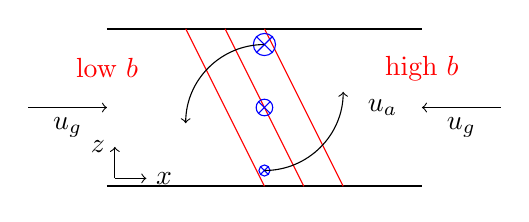
\begin{tikzpicture}		
				\draw[thick] (-2,0) -- (2,0);
				\draw[thick] (-2,2) -- (2,2);
				\draw[->] (-1.9, 0.1) -- (-1.5, 0.1) node[right] {$x$};
				\draw[->] (-1.9, 0.1) -- (-1.9, 0.5) node[left] {$z$};
				\draw[red] (0.5,0) -- (-0.5,2);
				\draw[red] (1,0) -- (0,2);
				\draw[red] (0,0) -- (-1,2);
				\draw[red] (-2, 1.5) node {low $b$};
				\draw[red] (2, 1.5) node {high $b$};
				\draw[blue] (0,1.8) node[cross=3.4pt,blue] {};
				\draw[blue] (0,1.8) circle (4pt);
				\draw[blue] (0,1) node[cross=2.6pt,blue] {};
				\draw[blue] (0,1) circle (3pt);
				\draw[blue] (0,0.2) node[cross=1.8pt,blue] {};
				\draw[blue] (0,0.2) circle (2pt);
				\draw[->] (0,1.8) arc (90:180:1);
				\draw[->] (0,0.2) arc (-90:0:1);
				\draw (1.5, 1) node {$\symbf{u}_a$};
				\draw[->] (3,1) -- (2,1) node[midway,below] {$\symbf{u}_g$};
				\draw[->] (-3,1) -- (-2,1) node[midway,below] {$\symbf{u}_g$};
			\end{tikzpicture}
		\end{center}
\end{enumerate}

The ageostrophic velocity $\symbf{u}_a$ can be found from the
\emph{Sawyer-Eliassen equation}. Ageostrophic strain adds to the background
strain.

\subsubsection{PV conservation in the Boussinesq equations}
Recall the Boussinesq primitive equations. The Navier-Stokes equations under
Boussinesq approximations are
\begin{equation}
	\frac{\partial \symbf{u}}{\partial t} + \symbf{u}\cdot \nabla \symbf{u} +
	f \hat{\symbf{k}} \times \symbf{u} = -\nabla p + \symbf{F}
\end{equation}
where $\symbf{F}$ is a generic frictional forcing, and $p$ is redefined to
absorb $\inv{\rho_0}$. In addition, we have the buoyancy conservation equation
\begin{equation}
	\frac{\partial b}{\partial t} + \symbf{u} \cdot \nabla b = D
\end{equation}
where $D$ is the \emph{diabatic heating/cooling} term. FInally, we have
incompressibility $\nabla \cdot \symbf{u} = 0$. We will assume $f$ is constant
in line with the traditional approximation. Taking the curl of Boussinesq NS
we have
\begin{equation}
	\frac{\diffD \symbf{\omega}}{\diffD t} = f\frac{\partial u}{\partial z} +
	\symbf{\omega} \cdot \nabla \symbf{u} + \nabla \times \symbf{F}
\end{equation}
Let $\symbf{\omega}_a = \symbf{\omega} + f\hat{\symbf{k}}$, called
\emph{absolute vorticity}. Then
\begin{equation}
	\frac{\diffD \symbf{\omega}_a}{\diffD t} = \symbf{\omega}_a \cdot \nabla
	\symbf{u} + \nabla \times \symbf{F} \label{eq:abs}
\end{equation}
Note that
\begin{equation}
	(\symbf{\omega}_a\cdot\nabla)\frac{\diffD b}{\diffD t} = \symbf{\omega}_a
	\cdot \frac{\diffD \nabla b}{\diffD t} + (\symbf{\omega}_a \cdot \nabla
	\symbf{u})\cdot\nabla b
\end{equation}
Now adding $\nabla b \cdot \eqref{eq:abs}$ we have
\begin{equation}
	\frac{\diffD}{\diffD t} (\symbf{\omega}_a \cdot \nabla b) =
	\symbf{\omega}_a \cdot \nabla D + \nabla b \cdot \nabla \times \symbf{F}
\end{equation}
In the absence of diabatic and frictional forcing, $\symbf{\omega}_a \cdot
\nabla b$ is conserved. We call $\symbf{\omega}_a \cdot \nabla b$ the
\emph{Ertel PV}.

\subsection{Internal waves \& instabilities in fronts}
Consider an unbounded fluid with uniform horizontal and vertical buoyancy
gradients:
\begin{equation}
	B = M^2 x + N^2 z
\end{equation}
where $M$ and $N$ are constant. This is the basic state buoyancy field. We
assume this buoyancy field is in thermal wind balance, so that the basic state
velocity is
\begin{equation}
	\frac{\diffd \mathcal{V}}{\diffd z} = \frac{M^2}{f}
\end{equation}

\begin{center}
	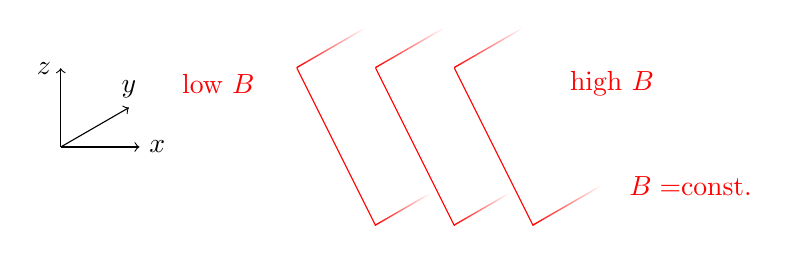
\begin{tikzpicture}
		\draw[red] (0, 1) -- (1, -1);
		\draw[red] (1, 1) -- (2, -1);
		\draw[red] (2, 1) -- (3, -1);
		\path[left color=red, right color=white,rotate around={30:(0,1)}]
		(0,1) rectangle +(1,.5pt);
		\path[left color=red, right color=white,rotate around={30:(1,1)}]
		(1,1) rectangle +(1,.5pt);
		\path[left color=red, right color=white,rotate around={30:(2,1)}]
		(2,1) rectangle +(1,.5pt);
		\path[left color=red, right color=white,rotate around={30:(1,-1)}]
		(1,-1) rectangle +(0.8,.5pt);
		\path[left color=red, right color=white,rotate around={30:(2,-1)}]
		(2,-1) rectangle +(0.8,.5pt);
		\path[left color=red, right color=white,rotate around={30:(3,-1)}]
		(3,-1) rectangle +(1,.5pt);
		\draw[red] (5, -0.5) node {$B = $const.};
		\draw[red] (-1, 0.8) node {low $B$};
		\draw[red] (4, 0.8) node {high $B$};
		\draw[->] (-3,0) -- (-2,0) node[right] {$x$};
		\draw[->] (-3,0) -- (-3,1) node[left] {$z$};
		\draw[->,rotate around={30:(-3,0)}] (-3,0) -- (-2,0) node[above] {$y$};
	\end{tikzpicture}
\end{center}

Consider the evolution of small perturbations to this basic state, denoted
$\symbf{u}, b, p$. We assume that these perturbations are independent of $y$,
the along-front direction. We also assume that the perturbations are
hydrostatic, that $f$ is constant, and we use the traditional approximation.
\lecture{18/11/20}
The linearised equations are
\begin{subequations}
	\begin{align}
	u_t - fv &= -p_x \label{eq:12.1a} \\
	v_t + w \frac{M^2}{f} + fu &= 0 \label{eq:12.1b} \\
	p_z &= b \label{eq:12.1c}\\
	b_t + wN^2 + uM^2 &= 0 \label{eq:12.1d}\\
	u_x + w_z &= 0 \label{eq:12.1e} \\
	\end{align}
\end{subequations}

We can eliminate variables in favour of $w$. Eliminate $v$ via
$\partial_t \eqref{eq:12.1a}$ and \eqref{eq:12.1b}:
\begin{equation}
	u_{tt} + wM^2 + uf^2 = -p_{xt} \label{eq:12.2}
\end{equation}
Eliminate $u$ via $\partial_x \eqref{eq:12.2}$ and \eqref{eq:12.1e}:
\begin{equation}
	-(\partial_t^2 + f^2)w_z + w_x M^2 = -p_{xxt} \label{eq:12.3}
\end{equation}
Eliminate pressure via $\partial_z \eqref{eq:12.3}$ and \eqref{eq:12.1c}:
\begin{equation}
	-(\partial_t^2 + f^2) w_{zz} + w_{xz} M^2 = -p_{xxzt} = -b_{xxt}
\end{equation}
Now $\partial_x \eqref{eq:12.1d}$ and $\eqref{eq:12.1e}$ gives
\begin{equation}
	b_{xt} + w_x N^2 - w_z M^2 = 0
\end{equation}
Hence we have
\begin{equation}
	(\partial_t^2 + f^2) w_{zz} + N^2 w_{xx} - 2M^2 w_{xz} = 0
\end{equation}
We now seek plane wave solutions with $w = \hat{w} e^{i(kx + mz - \omega t)}$
which gives dispersion relation
\begin{equation}
	\omega^2 = f^2 + \frac{k^2}{m^2} N^2 - 2\frac{k}{m} M^2 \label{eq:12dr}
\end{equation}
This is the dispersion relation for hydrostatic rotating stratified internal
waves modified by $M^2 = \frac{\partial B}{\partial x}$. Note: instability is
possible when $\omega^2 < 0$ if $M^2$ is large enough. Motivated by this, let
$\sigma \equiv -i\omega$ be the growth rate of the internal waves, then
\eqref{eq:12dr} gives
\begin{equation}
	\sigma^2 = -f^2 - N^2 \left( \frac{k}{m}-\frac{M^2}{N^2}\right)^2 +
	\frac{M^4}{N^2}
\end{equation}
The most unstable modes have $\frac{k}{m} = \frac{M^2}{N^2}$, in which case
the waves are aligned with surfaces of constant $B$.
\begin{center}
	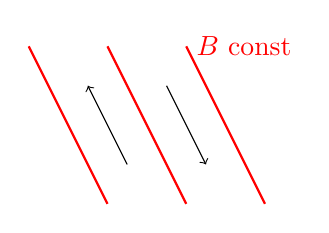
\begin{tikzpicture}
		\draw[red,thick] (0,0) -- (-1, 2);
		\draw[red,thick] (1, 0) -- (0, 2);
		\draw[red,thick] (2, 0) -- (1, 2) node[right] {$B$ const};
		\draw[->] (0.25, 0.5) -- (-0.25,1.5);
		\draw[<-] (1.25, 0.5) -- (0.75,1.5);
	\end{tikzpicture}
\end{center}

This is called \emph{symmetric instability} (SI). For $k/m = M^2/N^2$,
instability occurs if $\sigma^2 > 0$ which requires
\begin{equation}
	\frac{M^4}{N^2} - f^2 > 0
\end{equation}
or $\text{Ri} = N^2/(\frac{\diffd \mathcal{V}}{\diffd z})^2 < 1$ where
$\text{Ri}$ is the \emph{gradient Richardson number}.

The Ertel PV of the basic state is
\begin{equation}
	 q \equiv (f\hat{\symbf{k}} + \symbf{\omega})\cdot\nabla b = fN^2 -
	 \frac{M^4}{f}
 \end{equation}
 since $\symbf{\omega} = -M^2/f \hat{\symbf{x}}$. Symmetric instability
 develops if $fq < 0$. This is more general and holds for an unbalanced basic
 state too. This raises a paradox: symmetric instability requires $fq < 0$ to
 develop, but $q$ is conserved so remains negative. However, we know
 observationally that the instability does not grow indefinitely, so there
 must be some mechanism by which SI equilibriates. 
 
 \paragraph{How does $fq < 0$ develop?}
 Recall the Omega equation
 \begin{equation}
	 \frac{\diffD q}{\diffD t} = \symbf{\omega}_a \cdot \nabla D + \nabla b
	 \cdot \nabla \times \symbf{F} = \nabla \cdot (\symbf{\omega}_a D - \nabla
	 b \times \symbf{F})
 \end{equation}
since $\nabla \cdot \symbf{\omega}_a = 0$ and div curl vanishes. Consider the
region $0 \le z \le H$ and neglect horizontal fluxes.  Enforce boundary
conditions $w = 0$ on $z=0, H$. Then integrating the Omega equation we have
\begin{equation}
	\frac{\partial}{\partial t} \int_0^H \overline{q} \, \diffd z = \left[
		\overline{(\symbf{\omega}_a \cdot \hat{\symbf{k}})}D - \overline{\nabla b \times
	\symbf{F}}\cdot\hat{\symbf{z}}\right]_0^H
\end{equation}
where $\bar{.}$ denotes the horizontal average. For $\symbf{\omega}_a \cdot
\hat{\symbf{k}} > 0$, $\overline{q}$ decreases if
\begin{itemize}
	\item Convective forcing:
		\begin{itemize}
			\item $\left.D\right|_{z=H} < 0$ \,\,buoyancy loss due to cooling
			\item $\left.D\right|_{z=0} > 0$ \,\,buoyancy gain due to heating
		\end{itemize}
	\item Frictional forcing:
		\begin{itemize}
			\item $\nabla b \times \left.\symbf{F}\cdot\hat{\symbf{z}}\, \right|_{z=H} > 0$\,\,
					frictional stress aligned with thermal wind
			\item $\nabla b \times \left.\symbf{F}\cdot\hat{\symbf{z}} \,\right|_{z=H} < 0$\,\,
					frictional stress anti-aligned with thermal wind
		\end{itemize}
\end{itemize}

\begin{center}
	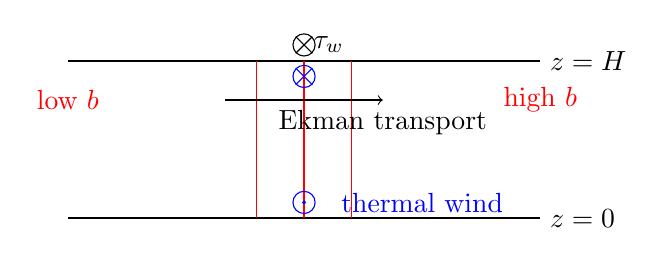
\begin{tikzpicture}
		\draw[thick] (-3, 0) -- (3,0);
		\draw[thick] (-3, 2) -- (3,2);
		\draw[red] (0.6, 0) -- (0.6, 2);
		\draw[red] (-0.6, 0) -- (-0.6, 2);
		\draw[red] (0, 0) -- (0, 2);
		\draw[red] (-3, 1.5) node {low $b$};
		\draw[red] (3, 1.5) node {high $b$};
		\draw (3,2) node[right] {$z=H$};
		\draw (3,0) node[right] {$z=0$};
		\draw[blue] (0,1.8) node[cross=3.4pt,blue] {};
		\draw[blue] (0,1.8) circle (4pt);
		\draw[blue] (0,0.2) circle (4pt);
		\draw[blue] (0,0.2) circle (0.5pt);
		\draw[blue] (1.5, 0.2) node {thermal wind};
		\draw[->] (-1, 1.5) -- (1, 1.5) node[below] {Ekman transport};
		\draw[black] (0,2.2) node[cross=3.4pt,black] {};
		\draw[black] (0,2.2) circle (4pt);
		\draw (0,2.2) node[right] {$\symbf{\tau}_w$};
	\end{tikzpicture}
\end{center}
		
\section{Mean Flows}
\lecture{20/11/20}
\subsection{Wave mean-flow interaction}
\subsubsection{Definitions}
We consider averages taken over $x$, and use the notation $\overline{(.)}$ to
denote the $x$-average, for example
\begin{equation}
	\overline{\chi} = \frac{1}{L} \int_0^L \chi \, \diffd x
\end{equation}
where the flow extends over $ 0 \le x \le L$. We typically assume periodicity
in $x$, motivated by atmospheric or circumpolar ocean geometry, with $x$
corresponding to longitude. Then we define $\chi' = \chi - \overline{\chi}$
with $\chi'$ often being alled the \emph{wave} or \emph{eddy} component. 
\begin{itemize}
	\item If the mean state is the background state then this matches the use
		of $(.)'$ in the derivation of the Boussinesq primitive equations.
		However, here the mean state may evolve in time whilst in the
		Boussinesq derivation the background state is typically
		time-independent.

	\item If periodicity in $x$ is assumed, then $\overline{\chi_x} = 0$.
		Hence $\overline{\theta_x \psi} = \overline{(\theta \psi)_x} -
		\overline{\theta \psi_x} = -\overline{\theta \psi_x}$. 

	\item Note that $\overline{(.)}$ is an Eulerian average, i.e. it is taken
		at fixed values of $y$ and $z$.
\end{itemize}

For convenience, henceforth we will drop the \,$\tilde{}$\, notation for $\rho$
and $p$ and these quantities will be interpreted respectively as the variation
of density and pressure away from the state with reference density
$\rho_s(z)$.

\subsubsection{Wave propagation and wave activity}
\paragraph{Dispersion relations.}
For plane waves, i.e. waves with sinusoidal structure in the spatial
coordinates $x, y, z$, or some subset of those coordinates, the dispersion
relation gives the frequency $\omega$ as a function of the spatial wavenumber
$\symbf{k}$. The phase velocity $\symbf{c}_p$ with components $\omega/k_i$ and
the group velocity $\symbf{c}_g$ with components $\partial \omega/\partial
k_i$ follow from the dispersion relation. Use of these various quantities
requires a \emph{scale separation} between the waves and the background
state, with the length scale of variation of the background state being much
larger than the wavelength.

\paragraph{Wave activity conservation relation.}
The wave activity conservation relation is an equation of the typical
conservation form
\begin{equation}
	\frac{\partial \mathcal{A}}{\partial t} + \nabla \cdot \symbf{F} =
	\mathcal{D}
\end{equation}
where $\mathcal{A}$ is the \emph{wave-activity density}, $\symbf{F}$ is a flux
and $\mathcal{D}$ is a term representing dissipation of wave activity, which
is associated with physical processes that are dissipative or otherwise
non-conservative.

We may derive this relation from the QG equations, starting from the QGPV
equation \eqref{eq:QGPVlin} linearised about a basic state flow in the $x$
direction. Denote the $x$ component of the velocity $\overline{u}$ and the
corresponding gradient of QGPV in the $y$ direction $\overline{q}_y$. This
implies that the instantaneous $x$-average can be considered a basic state,
whereas in \eqref{eq:QGPVlin} we have assumed the basic state is a
self-consistent steady solution of the QG equations. This inconsistency is
reolved by assuming that any time evolution of $\overline{u}, \overline{q}$ is
slow.

We may re-write \eqref{eq:QGPVlin} as
\begin{equation}
	\frac{\partial q'}{\partial t} + \overline{u} \frac{\partial q'}{\partial
	x} + v' \overline{q}_y = \mathcal{D}'
\end{equation}
where $\mathcal{D}'$ represents the effect of dissipation on $q'$. Multiplying
by $q'/\overline{q}_y$, assuming that $\overline{q}_y$ varies slowly in
time, and taking the $x$-average gives
\begin{equation}
	\frac{\partial}{\partial t}\left[ \frac{1}{2}
		\frac{\overline{q'^2}}{\overline{q}_y}\right] +\overline{v'q'} =
		\frac{\overline{q' \mathcal{D}'}}{\overline{q}_y}
		\label{eq:13.1}
\end{equation}

We now use the \emph{generalised Taylor identity} which follows from
multiplying $q'$ by $v'$:
\begin{align}
	v'q' &= \psi'_x \left(\psi'_{xx} + \psi'_{yy} + \left(\psi'_z
	\frac{f_0^2}{N^2}\right)_z\right) \\
	&= \left( \frac{1}{2} (\psi'_x)^2\right)_x + \left(\psi'_x\psi'_y\right)_y -
	\left(\frac{1}{2}(\psi'_y)^2\right)_x + \left( \psi'_x \psi'_z
		\frac{f_0^2}{N^2} \right)_z - \left(\frac{1}{2}(\psi'_z)^2
	\frac{f_0^2}{N^2}\right)_x
\end{align}

Taking the $x$-average of the above and subtitution into \eqref{eq:13.1} gives
\begin{equation}
	\frac{\partial}{\partial t}\left[ \frac{1}{2}
		\frac{\overline{q'^2}}{\overline{q}_y}\right] +
		\frac{\partial}{\partial y} \left[ -\overline{u'v'}\right] +
		\frac{\partial}{\partial z} \left[ -\frac{gf_0}{\rho_0N^2}
		\overline{v'\rho'}\right]	
		= \frac{\overline{q' \mathcal{D}'}}{\overline{q}_y}
\end{equation}

Note that the terms within the $y$ and $z$ derivatives have been re-expressed
in terms of $u', v'$ and $\rho'$. This equation has the structure
\begin{equation}
	\frac{\partial \overline{\mathcal{A}}}{\partial t} + \frac{\partial
		\overline{F^{(y)}}}{\partial y} + \frac{\partial
	\overline{F^{(z)}}}{\partial z} = \overline{\mathcal{D}_{\mathcal{A}}}
\end{equation}
which expresses the fact that $\overline{\mathcal{A}}$ is the density of a
quantity that can be transported by a flux with components $\overline{F^{(y)}}
$ and $\overline{F^{(z)}}$ in the $y$ and $z$ directions and destroyed or
created at a rate $\overline{\mathcal{D}_{\mathcal{A}}}$ per unit volume.
Here, $\overline{\mathcal{A}}$ is the \emph{Eliassen-Palm wave activity} and
$\overline{\symbf{F}}$ is the \emph{Eliassen-Palm flux}. This conservation relation
need not require a scale-separation assumption, but it is helpful if the
conservation relation is consistent with the cases where there is
scale-separation, in the sense that is then satisfies the
\emph{group-velocity} property $\langle \symbf{F}\rangle = \langle
\mathcal{A}\rangle \symbf{c}_g$ where $\langle \cdot \rangle$ denotes a phase
average. The Eliassen-Palm wave activity and flux satisfy this property.

\paragraph{Eddy fluxes and wave propagation.} The flux $\symbf{F}$ associates
correlations between different wave or eddy quantities with directions of wave
propagation. The Eliassen-Palm flux $y$-component $\overline{F^{(y)}} =
-\overline{u'v'}$ and the $z$-component $\overline{F^{(z)}} = -g f_0
\overline{v'\rho'}/N^2 \rho_0$ imply that the eddy flux in the $y$ direction
of the $x$-component of momentum $\overline{u'v'}$ satisfies
\begin{equation}
	\overline{u'v'} \begin{cases} < 0 & \text{for Northward group propagation}
		\\ > 0 & \text{for Southward group propagation}\end{cases}
\end{equation}

and that the eddy flux in the $y$ direction of the density
$\overline{v'\rho'}$ satisfies
\begin{equation}
	\overline{v'\rho'} \begin{cases}
		< 0 & \text{for upward group propagation} \\
		> 0 & \text{for downard group propagation}
	\end{cases}
\end{equation}

Note that these results hold for Rossby waves under the small $\Ro$ assumption
and also assuming that the $y$-gradient of PV in the basic state is positive,
as is always the case in the real atmosphere or ocean if this gradient is
dominated by $\beta$. For other waves (e.g. Poincar\'{e} waves), internal
waves or equatorial waves) the results are different.

\subsubsection{Mean-flow evolution equations}
Using the division into `mean' and `eddy' parts, we may apply the averaging
operator to the Boussinesq $\beta$-plane primitive equations to give
\begin{align}
	\overline{u}_t + (\overline{uv})_y + (\overline{uw})_z
	-\overline{v}(f_0+\beta y) &= 0 \\
	\overline{v}_t + (\overline{v^2})_y + (\overline{wv})_z + (f_0 + \beta y)
	\overline{u} &= -\frac{\overline{p}_y}{\rho_0} \\
	-\overline{p}z - \overline{\rho} g &= 0 \\
	\overline{v}_y + \overline{w}_z &= 0 \label{eq:13.6}\\
	\overline{\rho}_t + (\overline{\rho v})_y + (\overline{\rho w})_z &= 0
\end{align}

Note that to derive the above it is necessary to use the non-divergence of the
velocity field. The simplest approach is to re-write $\frac{\diffD u}{\diffD
	t}$ as $u_t + (u^2)_x + (uv)_y + (uw)_z$ and similarly for $\frac{\diffD
v}{\diffD t}$ and $\frac{\diffD \rho}{\diffD t}$. 

The definition of the averaging operator as well as \eqref{eq:13.6} gives
\begin{equation}
	(\overline{uv})_y + (\overline{uw})_z = (\overline{u}\overline{v})y +
	(\overline{u}\overline{v})_z + (\overline{u'v'})_y + (\overline{u'w'})_z =
	\overline{v}\overline{u}_y + \overline{w}\overline{u}_z +
	(\overline{u'v'})_y + (\overline{u'w'})_z
\end{equation}
Note the primes denote disturbances from the $x$-average. Now applying the
small $\Ro$ scaling, dividing horizontal velocities into geostrophic and
ageostrophic components and noting that $\overline{v}_g$ is zero, we have
\begin{align}
	\overline{u}_t - f_0 \overline{v}_a &= -(\overline{u'v'})_y
	\label{eq:13.8}\\
	f_0 \overline{u} &= -\frac{\overline{p}_y}{\rho_0} \label{eq:13.9}\\
	-\overline{p}_z - \overline{\rho}g &= 0 \label{eq:13.10}\\
	\overline{v}_{ay} + \overline{w}_{az} &= 0 \label{eq:13.11}\\
	\overline{\rho}_t + \overline{w}_a \frac{\diffd \rho_s}{\diffd z} &=
	-(\overline{\rho' v'})_y\label{eq:13.12}
\end{align}
This is a coupled set of equations for the five Eulerian-mean quantities
$\overline{u}_t, \overline{\rho}_t, \overline{p}, \overline{v}_a,
\overline{w}_a$, where the lack of subscript on $u, v$ implies the geostrophic
components.

There are two \emph{eddy forcing} terms $-(\overline{u'v'})_y$ and
$-(\overline{\rho'v'})_y$, determined respectively by the eddy momentum flux
and the eddy density (or heat) flux. 

\subsubsection{Transformed Eulerian mean equations}
We now make a transformation $\overline{w}_a \to \overline{w}_a^*$ defined by
\begin{equation}
	\overline{w}_a^* = \overline{w}-a + \frac{(\overline{\rho' v'})_y}{\diffd
	\rho_s / \diffd z}
\end{equation}
and define $\overline{v}_a^*$ such that 
\begin{equation}
	\overline{w}_{az}^* + \overline{v}_{ay}^* = 0 \label{eq:13.14}
\end{equation}
Hence we have
\begin{equation}
	\overline{v}_a^* = \overline{a}_a - \frac{\partial}{\partial z} \left[
	\frac{\overline{\rho' v'}}{\diffd \rho_s/\diffd z}\right]
\end{equation}
The $x$-momentum and density equations then become
\begin{align}
	\overline{u}_t - f_0 \overline{v}_a^* &= -(\overline{u'v'})_y + \left(
	\frac{f_0 \overline{\rho'v'}}{\diffd \rho_s/\diffd z}\right)_z = \nabla
	\cdot \overline{\symbf{F}} \label{eq:13.16}\\
	\overline{\rho}_t + \overline{w}_a^* \frac{\diffd \rho_s}{\diffd z} &=
	0\label{eq:13.17}
\end{align}

These two equations combined with \eqref{eq:13.9}, \eqref{eq:13.10},
\eqref{eq:13.14} are the \emph{transformed Eulerian mean equations}. The
transformation has combined the two separate eddy forcing terms into a single
term $\nabla \cdot \overline{\symbf{F}}$ in the $x$-momentum equation and has
removed the eddy forcing terms in the density equation. Note
$\overline{\symbf{F}}$ is the Eliassen-Palm flux vector and here $\nabla \cdot
\overline{\symbf{F}}$ is interpreted as the force acting on the mean flow due
to the eddies. 

The transformation does not change the response of $\overline{u}_t$ or
$\overline{\rho}_t$, but the eddy density flux appears to play a different
role. In the standard Eulerian-mean formalism the density flux
$\overline{\rho'v'}$ appears as a forcing in the density equation, whilst here
it is part of the force, and in fact $f_0 \overline{\rho'v'}/(\diffd
\rho_s/\diffd z)$ appears to act as a vertical momentum flux. Hence in the
transformed Eulerian-mean formalism, just as horizontally propagating Rossby
waves transfer momentum in the horizontal, vertically propagating Rossby waves
can be considered to transfer momentum in the vertical.

Note that the Eulerian-mean circulation and the transformed Eulerian-mean
circulation satisfy different boundary conditions.

\lecture{23/11/20}
\subsubsection{Non-acceleration conditions}
The divergence of the mean Eliassen-Palm flux $\nabla \cdot
\overline{\symbf{F}}$ appear as the complete eddy forcing on the mean flow. We
also have the Eliassen-Palm wave activity conservation relation
\begin{equation}
	\frac{\partial \mathcal{A}}{\partial t} + \nabla \cdot \symbf{F} =
	\mathcal{D}
\end{equation}
from which we deduce
\begin{equation}
	\nabla \cdot \overline{\symbf{F}} = \overline{\mathcal{D}} -
	\frac{\partial \mathcal{A}}{\partial t}
\end{equation}
It follows that if $\mathcal{A}_t = 0$, i.e. the waves are steady, and
$\mathcal{D} = 0$, i.e. there are no dissipative or other non-conservative
effects, then $\nabla \cdot \overline{\symbf{F}} = 0$ and hence
$\overline{u}_t = 0$, i.e. there is no acceleration of the mean flow. This is
called a \emph{non-acceleration theorem}. These theorems focus attention on
what is needed for there to be a mean flow acceleration.

Note that what is referred to as wave dissipation here may correspond to a
range of physical effects, including explicitly dissipative processes such as
viscosity or some other frictional effect, thermal or molecular or density
diffusion, or other thermal damping acting on their own. It may be that the
waves \emph{break}, i.e. they become strongly non-linear, generating
turbulence and hence adding to the dissipative processes that would have
otherwise been weak.

Under geostrophic scaling, we can show that
\begin{equation}
	\nabla \cdot \overline{\symbf{F}} = \overline{v'q'}
\end{equation}
where the right-hand quantity is the northward latitudinal flux of QGPV.
Similarly, we could quantity the effect of eddies on the mean flow via the
QGPV equation, now taking the form
\begin{equation}
	\overline{q}_t + (\overline{v'q'})_y = 0
\end{equation}
The mean acceleration $\overline{u}_t$ and the rate of change of mean density
$\overline{\rho}_t$ could then be deduced by using the appropriate inversion
operator. An advantaghe of using the transformed Eulerian-mean equations is
the response in the mean circulation $(\overline{v}_a^*, \overline{w}_a^*)$ is
explicitly visible.

\subsubsection{Wave dissipation}
Consider two-dimensional flow on a $\beta$-plane, governed by the QGPV
equation for a single-layer with the deformation radius $L_d \to \infty$, with
waves propagating in the $y$-direction. The \emph{absolute vorticity}
$\zeta_a$ is the sum of the relative vorticity $\zeta$ and the $\beta y$ term
which is materially conserved in the absence of dissipation.

\begin{itemize}
	\item In the case of no dissipation, i.e. $\mathcal{D} = 0$, then as a 
		wavepacket propagates through a region, $\frac{\partial
		\mathcal{A}}{\partial t} > 0$ when it arrives, so $\nabla \cdot
		\bar{\symbf{F}} > 0$. As the wavepacket leaves the region,
		$\frac{\partial \mathcal{A}}{\partial t} < 0$ hence $\nabla \cdot
		\bar{\symbf{F}} < 0$. The force on the mean flow is first
		negative, then positive, so the time-integrated force is zero. Hence
		the waves have no net effect on the mean flow.
		\begin{center}
			\begin{tikzpicture}[scale=1.5]
				\draw[->] (-0.1, 0) -- (5, 0) node[right] {$t$};
				\draw[->] (0, -0.1) -- (0, 2) node[left] {$\mathcal{A}$};
				\draw[smooth,blue] plot[domain=0:5] ({\x},{1.6*exp(-2*(\x-2)*(\x-2))});
				\draw (1, -0.5) node {$\frac{\partial \mathcal{A}}{\partial t} > 0$};
				\draw (3, -0.5) node {$\frac{\partial \mathcal{A}}{\partial t} <0$};
				\draw (0.8, 1) node {$\nabla \cdot \bar{\symbf{F}} < 0$};
				\draw (3.2, 1) node {$\nabla \cdot \bar{\symbf{F}} > 0$};
			\end{tikzpicture}
		\end{center}
	\item When dissipation is present, the wave arrives with $\frac{\partial
		\mathcal{A}}{\partial t} > 0$ and hence $\nabla \cdot
		\bar{\symbf{F}} < 0$ as before. As the wave dissipates,
		$\frac{\partial \mathcal{A}}{\partial t} = \mathcal{D} < 0$ and
		hence $\nabla \cdot \hat{\symbf{F}} = 0$. Therefore a net negative
		force is applied to the mean flow.
		\begin{center}
			\begin{tikzpicture}[scale=1.5]
				\draw[->] (-0.1, 0) -- (5, 0) node[right] {$t$};
				\draw[->] (0, -0.1) -- (0, 2) node[left] {$\mathcal{A}$};
				\draw[smooth,blue] plot[domain=0:2.3] ({\x},{1.6*exp(-2*(\x-2)*(\x-2))});
				\draw[smooth,blue] plot[domain=2.3:5] ({\x},{1.34*exp(-(\x-2.3))});
				\draw (1, -0.5) node {$\frac{\partial \mathcal{A}}{\partial t} > 0$};
				\draw (3, -0.5) node {$\frac{\partial \mathcal{A}}{\partial t}
				= \mathcal{D} <0$};
				\draw (0.8, 1) node {$\nabla \cdot \bar{\symbf{F}} < 0$};
				\draw (3.2, 1) node {$\nabla \cdot \bar{\symbf{F}} = 0$};
			\end{tikzpicture}
		\end{center}
\end{itemize}

Hence for there to be a net effect on the mean flow in some region, the waves
must arrive but not leave, e.g. through dissipation.

\paragraph{Rossby wave critical layer.} Consider a forced Rossby wave on a
shear flow $U(y)$. The equation describing the Rossby waves is
\eqref{eq:QGPVlin} and we assume a plane-wave form $\psi' = \hat{\psi}(y)
e^{ik(x-ct)}$. The equation for $\hat{\psi}(y)$ is then
\begin{equation}
	(U-c)(\hat{\psi}_{yy}-k^2\hat{\psi}) + (\beta-U_{yy})\hat{\psi} = 0
\end{equation}

The regions where $U = c$ are called \emph{critical lines}. The sign of
$\hat{\psi}_{yy}/\hat{\psi}$ changes from one side of the critical line to the
other, so that on one side waves propagate and on the other the waves are
evanescent. The equation is singular at $U = c$ hence there is no possible
steady linear non-dissipative balance and our governing equation is
insufficient. This small but finite region about the critical line is the
\emph{critical layer}. In a configuarion where the waves are generated away
from the critical line and propagate towards it, they dissipate near the
critical layer which implies a systematic force is applied to the flow in the
critical layer. There may be some reflection by this critical layer, but this
can only be determined by considering the detailed dynamics in this layer.

\begin{center}
	\begin{tikzpicture}[scale=2]
		\draw[dashed] (-3, 0) -- (3, 0);
		\draw[smooth] plot[domain=-3:3] ({\x},{0.2*sin(2*deg(\x))});
		\draw[smooth] plot[domain=-3:3] ({\x},{-0.2*sin(2*deg(\x))});
		\draw[smooth] plot[domain=-3:3] ({\x},{-0.3-0.1*sin(4*deg(\x)-90)});
		\draw[smooth] plot[domain=-3:3] ({\x},{-0.6-0.05*sin(4*deg(\x)-90)});
		\draw[smooth] plot[domain=-3:3] ({\x},{-0.9-0.02*sin(4*deg(\x)-90)});
		\draw[smooth] plot[domain=-3:3] ({\x},{0.3+0.1*sin(4*deg(\x)-90)});
		\draw[smooth] plot[domain=-3:3] ({\x},{0.9+0.1*sin(4*deg(\x)-120)});
		\draw[smooth] plot[domain=-3:3] ({\x},{1.5+0.1*sin(4*deg(\x)-150)});
		\draw[smooth] plot[domain=-3:3] ({\x},{2.1+0.1*sin(4*deg(\x)-180)});
		\draw[->] (0.785,0) [partial ellipse=90:-90:0.3 and 0.1];
		\draw[<-] (0.785,0) [partial ellipse=-270:-90:0.3 and 0.1];
		\draw[->] (-0.785,0) [partial ellipse=90:-90:0.3 and 0.1];
		\draw[<-] (-0.785,0) [partial ellipse=-270:-90:0.3 and 0.1];
		\draw[->] (2.356,0) [partial ellipse=90:-90:0.3 and 0.1];
		\draw[<-] (2.356,0) [partial ellipse=-270:-90:0.3 and 0.1];
		\draw[->] (-2.356,0) [partial ellipse=90:-90:0.3 and 0.1];
		\draw[<-] (-2.356,0) [partial ellipse=-270:-90:0.3 and 0.1];
		\draw[->] (0.784,0.2)--(0.786,0.2); 
		\draw[<-] (0.784,-0.2)--(0.786,-0.2); 
		\draw[<-] (-0.784,0.2)--(-0.786,0.2); 
		\draw[->] (-0.784,-0.2)--(-0.786,-0.2); 
		\draw[->] (2.355,0.2)--(2.357,0.2); 
		\draw[<-] (2.355,-0.2)--(2.357,-0.2); 
		\draw[<-] (-2.355,0.2)--(-2.357,0.2); 
		\draw[->] (-2.355,-0.2)--(-2.357,-0.2); 
		\draw[->] (0.784,0.4)--(0.786,0.4); 
		\draw[<-] (0.784,-0.4)--(0.786,-0.4); 
		\draw[<-] (-0.784,0.4)--(-0.786,0.4); 
		\draw[->] (-0.784,-0.4)--(-0.786,-0.4); 
		\draw[->] (2.355,0.4)--(2.357,0.4); 
		\draw[<-] (2.355,-0.4)--(2.357,-0.4); 
		\draw[<-] (-2.355,0.4)--(-2.357,0.4); 
		\draw[->] (-2.355,-0.4)--(-2.357,-0.4); 
		\draw[->] (0.915, 1) -- (0.917, 1);
		\draw[->] (0.915+1.57, 1) -- (0.917+1.57, 1);
		\draw[->] (0.915-1.57, 1) -- (0.917-1.57, 1);
		\draw[->] (0.915-3.14, 1) -- (0.917-3.14, 1);
		\draw[->] (1.046, 1.6) -- (1.048, 1.6);
		\draw[->] (1.046+1.57, 1.6) -- (1.048+1.57, 1.6);
		\draw[->] (1.046-1.57, 1.6) -- (1.048-1.57, 1.6);
		\draw[->] (1.046-3.14, 1.6) -- (1.048-3.14, 1.6);
		\draw[->] (1.177, 2.2) -- (1.179, 2.2);
		\draw[->] (1.177+1.57, 2.2) -- (1.179+1.57, 2.2);
		\draw[->] (1.177-1.57, 2.2) -- (1.179-1.57, 2.2);
		\draw[->] (1.177-3.14, 2.2) -- (1.179-3.14, 2.2);
		\draw[->] (0.01,-0.55) -- (-0.01,-0.55);
		\draw[->] (0.01,-0.88) -- (-0.01,-0.88);
		\draw[->] (1.57+0.01,-0.55) -- (1.57-0.01,-0.55);
		\draw[->] (1.57+0.01,-0.88) -- (1.57-0.01,-0.88);
		\draw[->] (-1.57+0.01,-0.55) -- (-1.57-0.01,-0.55);
		\draw[->] (-1.57+0.01,-0.88) -- (-1.57-0.01,-0.88);
		\draw[smooth,blue,thick,->] plot[domain=2.5:1.3352,variable=\y]
		({1+0.05*sin(20*deg(\y))},{\y});
		\draw[smooth,blue,thick,->] plot[domain=2.5:1.3352,variable=\y]
		({-1+0.05*sin(20*deg(\y))},{\y});
		\draw[smooth,blue!50,<-] plot[domain=2.0159:0.8,variable=\y]
		({1.2+0.05*sin(20*deg(\y)-60)},{\y});
		\draw[smooth,blue!50,<-] plot[domain=2.0159:0.8,variable=\y]
		({-0.8+0.05*sin(20*deg(\y)-60)},{\y});
		\draw (0, 2.5) node[blue] {Rossby waves};
		\draw (-3.5, 0.1) node {Critical};
		\draw (-3.5, -0.1) node {layer};
		\draw (-3.6, 1.7) node[left,rotate=90] {Wave};
		\draw (-3.4, 2) node[left,rotate=90] {propagation};
		\draw (-3.6, -0.7) node[left,rotate=90] {Wave};
		\draw (-3.4, -0.4) node[left,rotate=90] {evanescence};
		\draw[thick,->] (3.2,0) -- (4, 0) node[right] {$U(y)$};
		\draw[thick,->] (3.6, -2) -- (3.6, 2.5) node[left] {$y$};
		\draw[blue] (3.28, -2) -- (4, 2.5);
		\draw[blue!80,->] (3.6, 1) -- (3.75, 1);
		\draw[blue!80,->] (3.6, -1) -- (3.45, -1);
		\draw[blue!80,->] (3.6, 2) -- (3.92, 2);
		\draw[blue!80,->] (3.6, -1.8) -- (3.32, -1.8);
	\end{tikzpicture}
\end{center}

\paragraph{Rearrangement of absolute vorticity.}
When non-linearity is an important part of the processes in the critical layer
then the effect may be understood in terms of rearrangement of the
pre-existing absolute vorticity profile, which may be understood as `wave
breaking'. In the model problem above, the rearrangement occurs in a
\emph{non-linear critical layer} centred about $y=0$ through advection around
the `cat's eye' streamlines.

A simple model is to suppose that before the waves arrive, the absolute
vorticity is $\zeta_a = \beta y$ everywhere and after the waves have arrived
the absolute vorticity is \emph{mixed} within some region $\abs{y} < \delta$
to be equal to zero, the average value before the waves arrived. 
\begin{center}
	\begin{tikzpicture}
		\draw[thick,->] (-3, 0) -- (3, 0) node[right] {$\zeta_a$};
		\draw[thick,->] (0, -2) -- (0, 2) node[left] {$y$};
		\draw[dashed] (-2,-2) -- (2, 2) node[right] {$\zeta_a = \beta y$};
		\draw[blue] (-2, -2) -- (-1, -1) -- (0, -1) -- (0, 1) -- (1,1) --
		(2,2);
		\draw (-0.1, -1) -- (0.1, -1) node[right] {$y = -\delta$};
		\draw (0.1, 1) -- (-0.1, 1) node[left] {$y = \delta$};
	\end{tikzpicture}
\end{center}

Hence the change in relative vorticity $\zeta = -\beta y$ in $\abs{y} <
\delta$ and, assuming that the change in the $x$-component of velocity $\Delta
u$ is zero outside of $\abs{y} < \delta$, then we have
\begin{equation}
	\Delta u = \frac{\beta}{2}(y^2-\delta^2)
\end{equation}
in $\abs{y} < \delta$. The change in the $x$-momentum within this region is
thus
\begin{equation}
	\int_{-\delta}^\delta \Delta u \, \diffd y = -\frac{2}{3}\beta \delta^3
\end{equation}
Note the rearrangement of absolute vorticity does not \emph{locally} conserved
momentum -- an external force is required -- but this force is suppled by the
transport of momentum by the waves.

\subsubsection{Summary}
Two important general principles on wave propagation and wave mean-flow
interaction are:
\begin{enumerate}
	\item There can be long-range transfer of momentum. Propagating waves
		transfer momentum from the region where they are generated to the
		region where they dissipate or break.
	\item Dissipating or breaking waves change the potential vorticity
		distribution in the region where dissipation of breaking occurs. This
		change is not usually consistent with local conservation of momentum,
		but is consistent with the long-range transfer of momentum by the
		waves into or out of the region, i.e. total conservation of momentum.
\end{enumerate}

\paragraph{Mean-flow interaction problem subtleties.}
We have established that $\overline{u}_t = -(\overline{u'v'})_y$ (and
corresponding expressions in the 3D case), but the most difficult part of the
wave mean-flow interaction problem is to predict the dependence of
$\overline{u'v'}$ on $\overline{u}$. Ideally, $\overline{u'v'} =
\mathcal{F}\!\left[\overline{u}\right]$ for some $\mathcal{F}$ which we could
then solve for the evolution of $\overline{u}$. The functional $\mathcal{F}$
must incorporate the effects of flow-dependent wave propagation and
flow-dependent trajnsport of potential vorticity. For example, down-gradient
diffusion of momentum is a poor model for $\mathcal{F}$ since Rossby waves
generated where the flow is strong and positive and dissipating where the flow
is weak imply a wave activity flux from the strong-flow region to the
weak-flow region. Hence there is a momentum flux from the weak-flow region to
the strong-flow region, i.e. momentum transport \emph{up} the gradient. 

\paragraph{Mean-flow \& baroclinic instability.}
The choice of $\mathcal{F}$ is particularly important in understanding the
effect of baroclinic instability on the mean flow. From our previous
discussion of the Eady problem, we know $\overline{\rho'v'} < 0$ for the
growing wave, and $\overline{u'v'} = 0$. Hence the Eliassen-Palm flux is
purely upward. In more complicated basic states with eastward jet-like
structure in the $y$ direction, $\overline{u'v'} \ne 0$ and the pattern of
$\overline{u'v'}$ implies wave-activity flux \emph{out} of the jet and hence
flux of eastward horizontal momentum \emph{into} the jet. Again, the momentum
flux is up-gradient. This is because the growing instability corresponds to a
\emph{source} of wave activity in the jet and hence wave propagation out of
the jet.

\subsection{Mean meridional circulations}
\lecture{25/11/20}
\subsubsection{Introduction}
We will examine in more detail the mean response of a fluid to wave forcing,
comparing the Eulerian-mean viewpoint expressed by the coupled set of
equations \eqref{eq:13.8}, \eqref{eq:13.9}, \eqref{eq:13.10},
\eqref{eq:13.11}, \eqref{eq:13.12}, and the transformed Eulerian-mean
viewpoint expressed by the coupled set of equations \eqref{eq:13.9},
\eqref{eq:13.10}, \eqref{eq:13.14}, \eqref{eq:13.16}, \eqref{eq:13.17}.

Each of the velocity fields $(\overline{v}_a, \overline{w}_a)$ and
$(\overline{v}_a^*, \overline{w}_a^*)$ represents a circulation in the
\emph{meridional} $(y,z)$ plane. Since each field is non-divergent we may
define streamfunctions $\overline{\chi}_a, \overline{\chi}_a^*$ such that
\begin{align}
	(\overline{v}_a, \overline{w}_a) &=
	(\overline{\chi}_{az},-\overline{\chi}_{ay}) \\
	(\overline{v}_a^*, \overline{w}_a^*) &=
	(\overline{\chi}_{az}^*,-\overline{\chi}_{ay}^*)
\end{align}

It may be shown from the Eulerian-mean and transformed Eulerian-mean equations
that
\begin{align}
	f_0^2 \overline{\chi}_{azz} + N^2 \overline{\chi}_{ayy} = f_0
	(\overline{u'v'})_{yz} - \frac{g}{\rho_0} (\overline{\rho'v'})_{yy} &= -f_0
	\overline{F^{(y)}}_yz + \frac{N^2}{f_0} \overline{F^{(z)}}_{yy}
	\label{eq:mmc_eul}\\
	f_0^2 \overline{\chi}_{azz}^* + N^2 \overline{\chi}_{ayy}^* = f_0
	(\overline{u'v'})_{yz} - f_0^2 \left( \frac{\overline{\rho'v'}}{\diffd
			\rho_s / \diffd z}\right)_{zz} &= -f_0 (\nabla \cdot
			\bar{\symbf{F}})_z\label{eq:mmc_teul}
\end{align}
where $\symbf{\bar{F}} = (0, \overline{F^{(y)}}, \overline{F^{(z)}})$ is
the $x$-averaged Eliassen-Palm flux. These equations express the forcing on
the mean meridional circulation by the eddy fluxes of momentum and density
(or, equivalently, by the EP flux divergence).

\subsubsection{Boundary conditions}
The equations \eqref{eq:mmc_eul} and \eqref{eq:mmc_teul} are supplemented by
boundary conditiosn on $\overline{\chi}_a$ or $\overline{\chi}_a^*$. The side
boundary condition is straightforward: e.g. $\overline{\chi}_{az} =
\overline{\chi}^*_{az} = 0$ at $y$-boundaries. The bottom boundary condition
requires care when deriving, particularly if the bottom is not flat. Consider
the case of topographic forcing at the lower boundary $z=h$ so that the full
non-linear boundary condition is
\begin{equation}
	w = \frac{\diffD h}{\diffD t}
\end{equation}
at $z=h(x,y,t)$ where $h$ is the \emph{topographic height}. If the topography
is small amplitude, we may use a Taylor series expansion to re-express the
full boundary condition in terms of quantities at $z=0$ rather than $z=h$:
\begin{equation}
	w+hw_z = h_t + uh_x + vh_y + u_z h h_x + v_z h h_y + \mathcal{O}(h^3)
\end{equation}
where all RHS quantities are now evaluated at $z=0$. Consider now the
continuity equation $u_x + v_y + w_z = 0$ from which we can use to write the
LHS as
\begin{equation}
	hw_z = -hu_x -hv_y = -(hu)_x - (hv)_y + h_x u + h_y v
\end{equation}
and substituting into the previous equation we have
\begin{equation}
	w = h_t + u_z h h_x + v_z h h_y + (hu)_x + (hv)_y + \mathcal{O}(h^3)
\end{equation}
We now assume that in the absence of topography the velocity is purely
longitudinal (i.e. $x$-direction), so that $v = \mathcal{O}(h)$ and
$\overline{h} = 0$ for all $t$. We may also replace $\overline{w}$ by
$\overline{w}_a$ in line with quasi-geostrophic scaling. Hence, taking
$x$-averages, at leading order we have
\begin{equation}
	\overline{w}_a(y,0,t) = (\overline{h'v'})_y
\end{equation}
Hence the Eulerian mean velocity does not necessarily vanish at $z=0$. The
corresponding boundary condition on the transformed Eulerian mean circulation
is
\begin{equation}
	\overline{w}_a^*(y,0,t) = (\overline{h'v'})_y +
	\frac{(\overline{\rho'v'})_y}{\diffd \rho_s/\diffd z}
\end{equation}

Assuming the waves are steady and there is no density dissipation at the lower
boundary, we may use $\frac{\diffD}{\diffD t} \rho(x,y,h,t) = 0$ to re-write
the lower boundary condition on $\rho$ as
\begin{equation}
	\overline{u}h'_x \frac{\diffd \rho_s}{\diffd z} = -\overline{u}\rho'_x -
	\psi'_x \overline{\rho}_y
\end{equation}

Now multiplying by $\psi'$ and averaging, it follows that $f_0
\overline{h'\psi'_x} = -\overline{F^{(z)}}$ and hence the lower boundary
condition on $\overline{w}_a$ and $\overline{w}_a^*$ may be written as
\begin{equation}
	\overline{w}_a = -\frac{1}{f_0} (\overline{F^{(z)}})_y \hspace{1em}
	\text{and} \hspace{1em} \overline{w}_a^* = 0 \hspace{1em}
	\text{on}\,\,\, z=0
\end{equation}
Note that it is the transformed Eulerian mean vertical velocity
$\overline{w}_a^*$ which vanishes at the lower boundary, and not
$\overline{w}_a$.

\subsubsection{Model problem}
Consider a flow at small $\Ro$ confined to a $\beta$-plane longitudinal
channel with rigid walls at $y=0, L$. Waves are forced by topographic
perturbations of the lower boundary of the form 
\begin{equation}
	h = \Re\left[ h_0 e^{ikx} \sin \frac{\pi y}{L}\right]
\end{equation}
The basic state flow is assumed to be in the $x$-direction, and the velocity a
function of height so $\symbf{u}= u_0(z)\symbf{\hat{x}}$. The vertical
variation of the waves depends on $u_0(z)$ and on the buoyancy frequency $N$.
Assuming $N$ is a function of $z$ only, as in quasi-geostrophic theory, then
we may write $\psi'$ as
\begin{equation}
	\psi' = \Re\left[ \hat{\psi}(z) e^{ikx} \sin \frac{\pi y}{L}\right]
\end{equation}
It follows that $\overline{\psi'_x\psi'_y} = 0$ so that the Eliassen-Palm flux
is purely vertical with
\begin{equation}
	\overline{F^{(z)}} = \frac{f_0^2}{N^2} \overline{\psi'_x\psi'_z} =
	\frac{f_0^2}{N^2} \Im \left[ k \hat{\psi}(z)^* \hat{\psi}'(z)\right]
	\sin^2 \frac{\pi y}{L} = F_0 \Theta(z) \sin^2 \frac{\pi y}{L}
\end{equation}
where $F_0 = f_0^2/N^2$ and $\Theta(z) = \Im \left[ k
\hat{\psi}^*\hat{\psi}'\right]$. To be consistent with the basic properties of
Rossby waves, for upward propagation we require $F_0 \Theta(z) > 0$. We can
determine $\Theta(z)$ by solving the equation for $\hat{\psi}(z)$ given the
$z$-variation of the basic state and of any dissipative processes. To avoid
this complication, we assume a simple step function form for $\Theta(z)$:
\begin{equation}
	\Theta(z) = \begin{cases} 1 & z < H_d \\ 0 & z > H_d \end{cases}
\end{equation}
This is a simple representation of a situation where waves are generated far
below $z=H_d$, propagate upwards, and dissipate in a thin critical layer
localised about $z=H_d$. The problem is then reduced to solving
\eqref{eq:mmc_eul} or \eqref{eq:mmc_teul} with a given forcing term and with
specified boundary conditions. The assumed form for $\overline{F^{(z)}}$ gives
a forcing term in \eqref{eq:mmc_eul} which is non-zero as $z \to -\infty$, but
a forcing term in \eqref{eq:mmc_teul} which tends to zero as $z \to \pm
\infty$. Thus it is more straightforward to solve \eqref{eq:mmc_teul} and seek
a solution $\overline{\chi}^*$ that tends to zero as $z \to \pm \infty$.
Once $\overline{\chi}^*$ is known, $\overline{\chi}$ may be deduced using the
inverse transformation.

The rigid wall boundary conditions imply $\overline{\chi}_{az} =
\overline{\chi}_{az}^*$ at $y=0,L$. It is therefore natural to expand the
forcing and solution in a sine Fourier series:
\begin{align}
	\overline{F^{(z)}} &= F_0 \Theta(z) \sum_{n=1}^\infty c_n \sin \frac{n \pi
	y}{L} \\
	\overline{\chi}_a^* &= \sum_{n=1}^\infty \overline{\chi}_n^*(z) \sin
	\frac{n \pi y}{L}
\end{align}
where the $c_n$ are the coefficients in the Fourier series for $\sin^2
\frac{\pi y}{L}$. The governing ODE for
$\overline{\chi}_n^*(z)$ follows from subtitution into \eqref{eq:mmc_teul}:
\begin{equation}
	f_0^2 \overline{\chi}_n^{*''}(z) - \frac{N^2 \pi^2 n^2}{L^2}
	\overline{\chi}_n^*(z) = f_0 F_0 c_n \delta'(z-H_d)
\end{equation}

The solution satisfying the boundary conditions $\overline{\chi}_n^* \to 0$ as
$z \to \pm \infty$ is
\begin{equation}
	\overline{\chi}_n^*(z) = \frac{F_0 c_n}{2f_0} \exp \left[ -\frac{N \pi
	n}{L f_0} \abs{z-H_d}\right] \text{sgn}(z-H_D)
\end{equation}
All flow variables can be deduced from the above solution. Using $(\cdot)_n$
to denote the $n$\textsuperscript{th} coefficient in the Fourier series, it
follows that
\begin{equation}
	(\overline{v}_a^*)_n = -\frac{F_0 c_n}{2f_0} \frac{N \pi n}{L f_0}
	\exp\left[ -\frac{N\pi n}{L f_0} \abs{z-H_d}\right] + \frac{F_0 c_n}{f_0}
	\delta (z-H_d)
\end{equation}
and, noting that $\nabla \cdot \hat{\symbf{F}} = -F_0 c_n \delta(z-H_d)$;
\begin{equation}
	(\overline{u}_t)_n = -\frac{F_0c_n}{2} \frac{N \pi n}{L f_0} \exp \left[
	-\frac{N \pi n}{L f_0} \abs{z-H_d}\right]
\end{equation}
Similar expressions may be derived for the Fourier coefficients of
$\overline{w}_a^*$ and $\overline{\rho}_t$. In particular, note
$\overline{\chi}_a = \overline{\chi}_a^* + \overline{F^{(z)}}/f_0$. We can
derive a schematic view of the response of various quantities to the eddy
forcing by considering only the $n=1$ Fourier coefficients. Gray shading
indicates negative values within solid lines, and positive values within
dashed lines.

\noindent
\makebox[1.3\textwidth][l]{
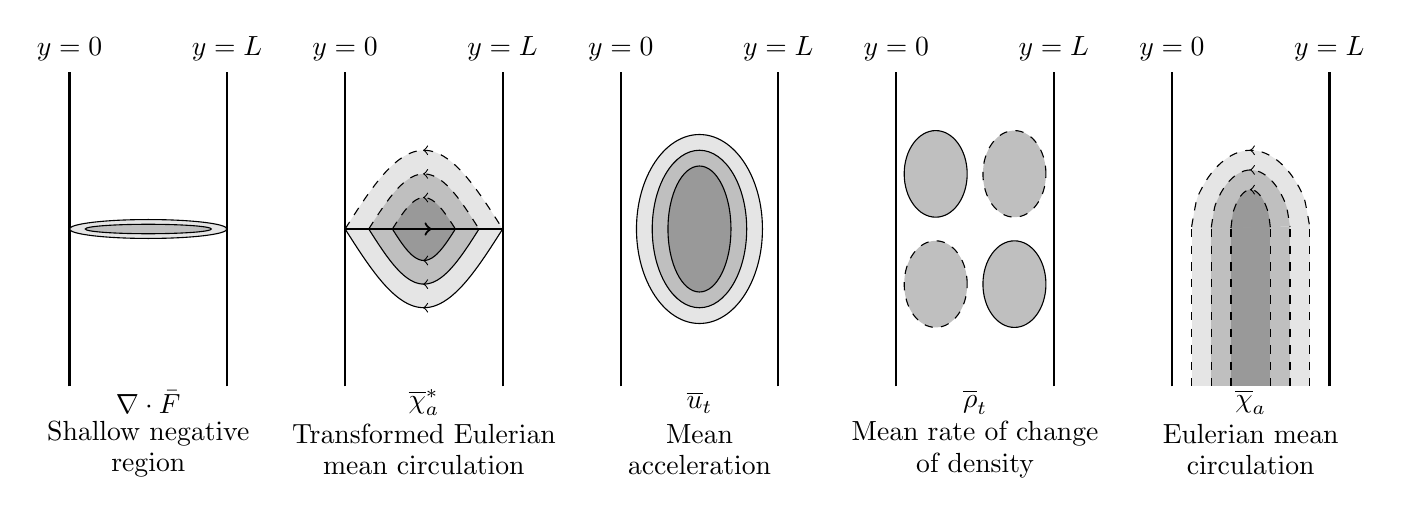
\begin{tikzpicture}
	\draw[thick] (-1,-2) -- (-1, 2) node[right,above] {$y=0$};
	\draw[thick] (1, -2) -- (1, 2) node[left,above] {$y=L$};
	\draw[fill=gray!20] (0,0) ellipse (1 and 0.12);
	\draw[fill=gray!50] (0,0) ellipse (0.8 and 0.06);
	\draw (0,-2.2) node {$\nabla \cdot \bar{\symbf{F}}$};
	\draw (0,-2.6) node {Shallow negative};
	\draw (0,-3) node {region};
	\begin{scope}[shift={(3.5,0)}]
	\draw[thick] (-1,-2) -- (-1, 2) node[right,above] {$y=0$};
	\draw[thick] (1, -2) -- (1, 2) node[left,above] {$y=L$};
	\draw[smooth,fill=gray!20,dashed] plot[domain=-1:1] ({\x},{cos(3.14*deg(\x)/2)});
	\draw[smooth,fill=gray!20] plot[domain=-1:1] ({\x},{-cos(3.14*deg(\x)/2)});
	\draw[smooth,fill=gray!50,dashed] plot[domain=-0.7:0.7] ({\x},
				{0.7*cos(3.14*deg(\x)/1.4)});
	\draw[smooth,fill=gray!50] plot[domain=-0.7:0.7] ({\x},
				{-0.7*cos(3.14*deg(\x)/1.4)});
	\draw[smooth,fill=gray!80,dashed] plot[domain=-0.4:0.4] ({\x},
				{0.4*cos(3.14*deg(\x)/0.8)});
	\draw[smooth,fill=gray!80] plot[domain=-0.4:0.4] ({\x},
				{-0.4*cos(3.14*deg(\x)/0.8)});
	\draw[thick] (-1,0) -- (1,0);
	\draw[thick,->] (-0.1,0) -- (0.1, 0);
	\draw[->] (0.01,1) -- (-0.01, 1);
	\draw[->] (0.01,0.7) -- (-0.01, 0.7);
	\draw[->] (0.01,0.4) -- (-0.01, 0.4);
	\draw[->] (0.01,-1) -- (-0.01, -1);
	\draw[->] (0.01,-0.7) -- (-0.01, -0.7);
	\draw[->] (0.01,-0.4) -- (-0.01, -0.4);
	\draw (0,-2.2) node {$\overline{\chi}_a^*$};
	\draw (0,-2.6) node {Transformed Eulerian};
	\draw (0,-3) node {mean circulation};
	\end{scope}
	\begin{scope}[shift={(7,0)}]
	\draw[thick] (-1,-2) -- (-1, 2) node[right,above] {$y=0$};
	\draw[thick] (1, -2) -- (1, 2) node[left,above] {$y=L$};
	\draw[fill=gray!20] (0,0) ellipse (0.8 and 1.2);
	\draw[fill=gray!50] (0,0) ellipse (0.6 and 1);
	\draw[fill=gray!80] (0,0) ellipse (0.4 and 0.8);
	\draw (0,-2.2) node {$\overline{u}_t$};
	\draw (0,-2.6) node {Mean};
	\draw (0,-3) node {acceleration};
	\end{scope}
	\begin{scope}[shift={(10.5,0)}]
	\draw[thick] (-1,-2) -- (-1, 2) node[right,above] {$y=0$};
	\draw[thick] (1, -2) -- (1, 2) node[left,above] {$y=L$};
	\draw[fill=gray!50,dashed] (0.5, 0.7) ellipse (0.4 and 0.55);
	\draw[fill=gray!50] (-0.5, 0.7) ellipse (0.4 and 0.55);
	\draw[fill=gray!50,dashed] (-0.5, -0.7) ellipse (0.4 and 0.55);
	\draw[fill=gray!50] (0.5, -0.7) ellipse (0.4 and 0.55);
	\draw (0,-2.2) node {$\overline{\rho}_t$};
	\draw (0,-2.6) node {Mean rate of change};
	\draw (0,-3) node {of density};
	\end{scope}
	\begin{scope}[shift={(14,0)}]
	\fill[gray!20] (-0.75,0.05) rectangle (0.75,-2);
	\fill[gray!50] (-0.5,0.05) rectangle (0.5,-2);
	\fill[gray!80] (-0.25,0.05) rectangle (0.25,-2);
	\draw[dashed] (-0.25,0) -- (-0.25,-2);
	\draw[dashed] (-0.5,0) -- (-0.5,-2);
	\draw[dashed] (-0.75,0) -- (-0.75,-2);
	\draw[dashed] (0.25,0) -- (0.25,-2);
	\draw[dashed] (0.5,0) -- (0.5,-2);
	\draw[dashed] (0.75,0) -- (0.75,-2);
	\draw[thick] (-1,-2) -- (-1, 2) node[right,above] {$y=0$};
	\draw[thick] (1, -2) -- (1, 2) node[left,above] {$y=L$};
	\draw[smooth,dashed,fill=gray!20] plot[domain=-0.75:0.75]
	({\x},{sqrt(cos(2*3.14*deg(\x)/3))});
	\draw[smooth,dashed,fill=gray!50] plot[domain=-0.5:0.5]
	({\x},{0.75*sqrt(cos(3.14*deg(\x)))});
	\draw[smooth,dashed,fill=gray!80] plot[domain=-0.25:0.25]
	({\x},{0.5*sqrt(cos(2*3.14*deg(\x)))});
	\draw[->] (0.01, 1) -- (-0.01, 1);
	\draw[->] (0.01, 0.75) -- (-0.01, 0.75);
	\draw[->] (0.01, 0.5) -- (-0.01, 0.5);
	\draw (0,-2.2) node {$\overline{\chi}_a$};
	\draw (0,-2.6) node {Eulerian mean};
	\draw (0,-3) node {circulation};
	\end{scope}
\end{tikzpicture}
}

Note the contrast between the responses in the transformed Eulerian-mean
circulation and the Eulerian-mean circulation and the implications for the
balance in the $x$-momentum and density equations.

\paragraph{Transformed Eulerian-mean view:} in the \emph{wave propagation}
region $z < H_d$ the vertical velocity $\overline{w}_a^*$ is zero and there is
vertical transport of momentum via $\overline{F^{(z)}}$. In the \emph{wave
dissipation} region centred on $z=H_d$ there is localised wave force $\nabla
\cdot \bar{\symbf{F}}$ which is redistributed in the vertical by the
meridional circulation $(\overline{v}_a^*, \overline{w}_a^*)$. 

\paragraph{Eulerian-mean view:} in the \emph{wave propagation} region $z <
H_d$ the vertical velocity $\overline{w}_a$ is non-zero. The effect of
$\overline{w}_a$ on the mean density field is cancelled by the effect of the
eddy flux $\overline{\rho'v'}$. There is vertical transport of planetary
angular momentum (because the fluid moving upwards on one side of the channel
has a different value of angular momentum to that moving downwards on the
other side of the channel). In the \emph{wave dissipation} region there is a
latitudinal velocity $\overline{v}_a$ which provides a Coriolis force and
hence leads to acceleration.

The transformed Eulerian-mean view is arguably simpler because it removes the
cancellation between the effect of vertical advection by the mean flow, and
the effect of eddy density fluxes. Also, it combines eddy fluxes into a single
forcing term as noted previously. Additionally it may be shown that the
transformed Eulerian-mean flow is more relevant to the transport of tracers.
Vertical motion in the Eulerian-mean circulation does not imply corresponding
vertical motion of tracers, e.g. the upward motion at high latitudes in the
`Ferrel cell' does not imply that tracers are transported upwards.

The transformed Eulerian-mean formalism can be interpreted as an approximation
to taking averages not at fixed $z$, but over very thin layers between
neighbouring density surfaces. The fact that the thickness and the
$z$-position of the layer are both variable affects the calculated average.
Momentum can be exchanged between neighbouring layers by pressure forces
acting on their boundaries.

\subsubsection{Dependence of response on vertical scale of $\nabla \cdot
\bar{\symbf{F}}$}
In the model problem above, $\nabla \cdot \bar{\symbf{F}}$ is non-zero only in
a layer with very small vertical scale. Suppose instead that the `forcing
layer' has vertical scale $D$. Then \eqref{eq:mmc_teul} gives
\begin{equation}
	\text{max} \left[ \frac{f_0^2 \overline{\chi}_a^*}{D^2}, \frac{N^2
	\overline{\chi}_a^*}{L^2}\right] \sim \frac{f_0 F_0}{D}
\end{equation}
The \emph{shallow forcing regime} is when $ND/f_0 L \ll 1$. Then $f_0^2
\overline{\chi}_a^* / D^2 \sim f_0 F_0/D$, hence $\overline{\chi}_a^* \sim F_0
D/f_0$ and $\overline{v}^*_a \sim F_0/f_0$. The dominant balance in the
momentum equations within the forcing layer is therefore that most of $\nabla
\cdot \bar{\symbf{F}}$ is balanced by the Coriolis force. THe mean meridional
circulation redistributes in the vertical the effect of $\nabla \cdot
\bar{\symbf{F}}$ and the resulting acceleration occurs over a region that is
much deeper than the forcing layer. 

The \emph{deep forcing regime} is when $ND/f_0 L \gg 1$. Then $N^2
\overline{\chi}_a^*/L^2 \sim f_0 F_0/D$, hence $\overline{\chi}_a^* \sim (f_0
L/ND)^2 F_0 D/f_0$ and $\overline{v}_a^* \sim (f_0 L /ND)^2 F_0/f_0$. The
Coriolis force therefore plays only a minor role in the momentum equation
within the forcing layer and at each level $\nabla \cdot \bar{\symbf{F}}$ is
balanced by the $x$-component of the mean acceleration.

The different regimes could be illustrated by replacing $\Theta(z)$ with a
simple function that varies from $1$ to $0$ over some finite vertical scale. 

\paragraph{Physical interpretation of mean meridional circulation.} The mean
meridional circulation may be regarded as arising in order to maintain, under
the effect of eddy forcing, the constraints of geostrophic and hydrostatic
balance. Thus if a force is applied to a rotating system, the response cannot
appear purely as an acceleration; there must be an accompanying change in the
density field. If a force is deep, in the sense given above, most of the
response will appear as acceleration. If the force, then most of the response
will appear as a meridional circulation and hence a density change. Similarly,
if an applied heating field is shallow, most of the response appears as a
change in temperature or density, but if it is deep, then most will appear as
meridional circulation, and hence as a change in velocity. 

\subsection{Equatorial waves}
\lecture{27/11/20}
Previously, we have considered wave motion when rotation and stratification
co-exist under the shallow-water model. The analysis gave Poincar\'{e} waves
and boundary Kelvin waves when $f = f_0$ is constant, and in the $\beta$-plane
approximation with $f = f_0 + \beta y$, Rossby waves. Poincar\'{e} and Kelvin
waves are `fast' waves whilst Rossby waves are `slow' waves since their
phase speed scale as $f_0 L_D, \beta L_D^2$ respectively. At low latitudes
when $\beta L_d \sim f_0$, this distinction is no longer clear. Dynamics at
low latitudes require a different analysis.

\subsubsection{Horizontal structure and propagation}
The shallow-water equations are still a suitable model for analysis at low
latitudes. The equatorial $\beta$-plane approximation is $f = \beta y$, i.e.
$f_0 = 0$ in the Coriolis parameter. Then the shallow-water equations
linearised about a state of rest are
\begin{align}
	u_t - \beta y v &= - g \eta_x \label{eq:sweq1} \\
	v_t + \beta y u &= - g \eta_y \label{eq:sweq2} \\
	\eta_t + H(u_x + v_y) &= 0\label{eq:sweq3}
\end{align}
where $u$ and $v$ the usual horizontal velocity components, $\eta$ is the free
surface displacement, and $H$ is the layer depth in the resting state.

There are two dimensional parameters present in these equations, $\beta$ and
$c = \sqrt{gH}$. These can be used to form time and lengthscales
$T_{\text{eq}} = (c\beta)^{_1/2}$ and $L_{\text{eq}} = (c/\beta)^{1/2}$.
$L_{\text{eq}}$ is referred to as the \emph{equatorial deformation radius},
the analogue of the extratropical deformation radius $L_D = c/f_0$. Taking
$\partial_x \eqref{eq:sweq2} - \partial_y \eqref{eq:sweq1} - \beta y
\eqref{eq:sweq3}$ gives
\begin{equation}
	\frac{\partial}{\partial t} (v_x - u_y - \frac{\beta y \eta}{H}) + \beta v
	= \frac{\partial}{\partial t} ( \zeta - \frac{\beta y \eta}{H}) + \beta v
	= 0 \label{eq:sweqpv}
\end{equation}
where $\zeta = v_x - u_y$ is the relative vorticity. This expresses
conservation of PV in the linearised approximation.

Now consider $\partial_t \eqref{eq:sweq2} - \beta y \eqref{eq:sweq1}$ which
gives
\begin{equation}
	v_{tt} + \beta^2 y^2 v = -g \eta_{yt} + \beta y g \eta_x
\end{equation}

Substitute for $\eta_t$ from \eqref{eq:sweq3} to get
\begin{equation}
	v_{tt} + \beta^2 y^2 v = gH (u_{xy} + v_{yy}) + \beta y g \eta_x = c^2
	(u_y - v_x + \frac{\beta y \eta}{H})_x + c^2 (v_{xx} + v_{yy})
\end{equation}
The first term includes the potential vorticity associated with the
disturbance, hence differentiate with respect to time and use
\eqref{eq:sweqpv} to get
\begin{equation}
	v_{ttt} + \beta^2 y^2 v_t - c^2 (v_{xx} + v_{yy})_t - \beta c^2 v_x = 0
\end{equation}

This equation is structurally similar to that obtained for the extratropics;
with $\beta y$ replaced by $f_0$ and the additional $\beta$ term eliminated
we obtain the equation for Poincar\'{e} waves in the extratropics. Seek plane
wave solutions of the form
\begin{equation}
	v = \Re\left[ \hat{v}(y) e^{i(kx-\omega t)} \right]
\end{equation}
with $k$ and $\omega$ the constant $x$-wavenumber and frequency respectively.
We require $\hat{v}(y)$ bounded as $\abs{y} \to \infty$. We find the ODE for
$\hat{v}$ as
\begin{equation}
	\left[ \frac{\omega^2}{c^2} - \frac{\beta^2 y^2}{c^2} - k^2 - \frac{\beta
	k}{\omega} \right] \hat{v} + \hat{v}_{yy} = 0
\end{equation}
This equation along with the boundary condition as $\abs{y} \to \infty$
defines an eigenvalue problem, yielding the eigenvalue condition
\begin{equation}
	\omega^2 - c^2 k^2 - \frac{\beta k c^2}{\omega} = (2n+1) \beta c
\end{equation}
for $n = 0, 1, 2, \dots$ with corresponding eigenfunctions
\begin{equation}
	\hat{v}_n(y) = H_n( y\sqrt{\beta/c}) e^{-\frac{y^2 \beta}{2c}}
\end{equation}
where $H_n$ are the \emph{Hermite polynomials} with $H_0(s) = 1, H_1(s) = 2s,
H_2(s) = 4s^2 - 2$, etc.

Non-dimensionalise the eigenvalue condition using $\omega T_{\text{eq}} =
\hat{\omega}$ and $k L_{\text{eq}} = \hat{k}$. Then
\begin{equation}
	\hat{\omega}^2 - \hat{k}^2 - \frac{\hat{k}}{\hat{\omega}} = 2n+1
\end{equation}
This is a quadratic for $\hat{k}$ given $\hat{\omega}$ with roots
\begin{equation}
	\hat{k} = -\frac{1}{2\hat{\omega}} \pm \sqrt{\hat{\omega}^2 +
	\frac{1}{4}\hat{\omega}^2 - (2n+1)}
\end{equation}

Note that for any pair $(\hat{k}, \hat{\omega})$, there is a corresponding
pair $(-\hat{k},-\hat{\omega})$ which represents the same wave mode. Hence it
is necessary to consider only half of the $(\hat{k}, \hat{\omega})$ plane and
by convention we choose $\hat{\omega} > 0, -\infty < \hat{k} < \infty$. 

\begin{itemize}
	\item The $n=0$ mode gives $\hat{k} = \hat{\omega} - 1/\hat{\omega}$ or
		$\hat{k} = -\hat{\omega}$. The second root is unphysical, so the $n=0$
		mode has dispersion relation
		\begin{equation}
			\hat{k} = \hat{\omega} - \frac{1}{\hat{\omega}}
		\end{equation}
		For $\hat{\omega} > 1$ we have $\hat{k} > 0$ and for $0 < \hat{\omega}
		< 1$ we have $\hat{k} < 0$.
	\item The $n = 1, 2, \dots$ modes have real roots only if $\hat{\omega}^4
		- (2n+1)\hat{\omega}^2 + \frac{1}{4\hat{\omega}^2} > 0$, implying
		either $\hat{\omega}^2 < n+\frac{1}{2}-\sqrt{n(n+1)}$ or
		$\hat{\omega}^2 > \sqrt{n(n+1)} + n + \frac{1}{2}$. Hence there is a
		frequency gap, the size of which increases with $n$.
\end{itemize}

This covers all solutions with $v \ne 0$. There are more solutions with $v =
0$ missed by the above approach. Setting $v=0$ in
\eqref{eq:sweq1}, \eqref{eq:sweq2}, \eqref{eq:sweq3} which yields $\eta_{tt} -
c^2 \eta_{xx} = 0$. Requiring exponential decrease in $y$ only (otherwise
unphysical) yields dispersion relation $\omega = ck$ for plane wave solutions
with
\begin{equation}
	\hat{\eta}(y) \propto e^{-\frac{\beta y^2}{2c}}
\end{equation}
This is an \emph{equatorial Kelvin wave} analogous to the boundary Kelvin wave
on an $f$-plane. There is no latitudinal velocity and the balance in the
latitudinal momentum equations is geostrophic between the Coriolis force
associated with $u$ and the pressure gradient associated with $\eta_y$. Note
that the relation $\omega = kc$ is equivalent to $\hat{\omega} = \hat{k}$ and
corresponds to the $n=-1$ mode of our previous dispersion relation.

\paragraph{Summary}
The equatorial wave modes can be split into the following types.
\begin{itemize}
	\item For $n = 1, 2, \dots$, for each $\omega > \sqrt{n(n+1)} + n +
		\frac{1}{2}$ there are two values of $\hat{k}$. These are high
		frequency \emph{Inertio-gravity / Poincar\'{e} waves}. Note in the
		large $\hat{k}$ regime these may be reffered to as gravity waves,
		whilst in the small $\hat{k}$ regime they may be reffered to as
		inertial waves.
	\item For $n = 1, 2, \dots$, there are also two values of $\hat{k}$ for
		each $\omega < n + \frac{1}{2} - \sqrt{n(n+1)}$ which are low
		frequency \emph{equatorial Rossby waves}.
	\item For $n = 0$ the dispersion relation $\hat{\omega} - 1/\hat{\omega} =
		\hat{k}$ is gravity-like $\hat{\omega} \sim \hat{k}$ as
		$\hat{k} \to \infty$ and Rossby-like $\hat{\omega} \sim 1/\hat{k}$ as
		$\hat{k} \to -\infty$. Hence the $n=0$ mode is referred to as a
		(mixed) \emph{Rossby-gravity wave}.
	\item The $n=-1$ mode with dispersion relation $\hat{\omega} = \hat{k}$ is
		an \emph{equatorial Kelvin wave}.
\end{itemize}

\begin{figure}
	\centering
	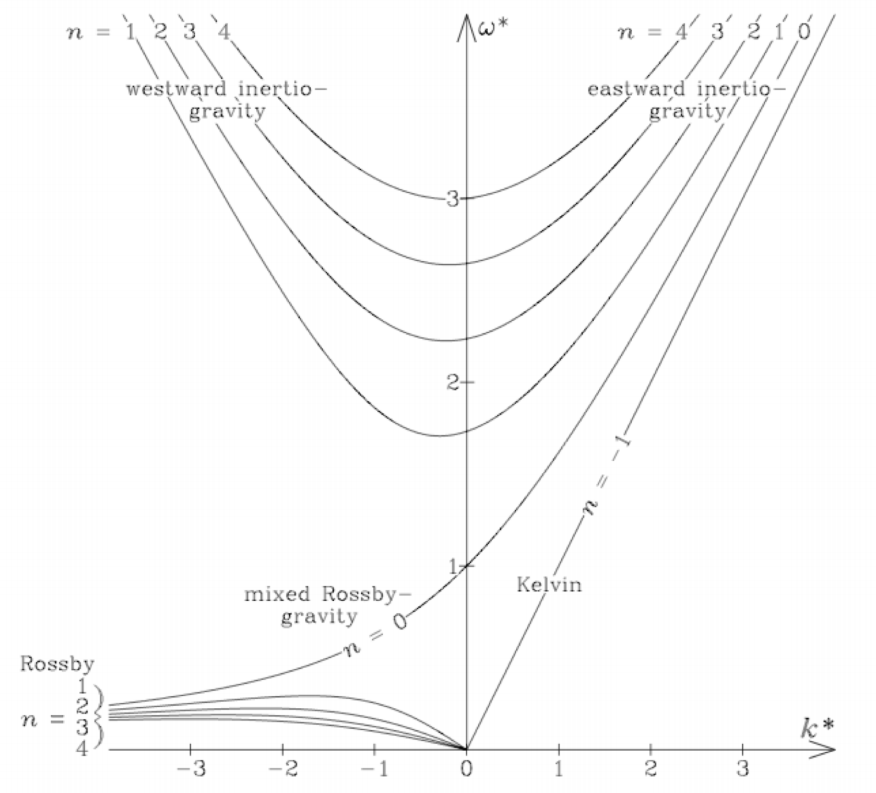
\includegraphics[width=0.7\textwidth]{equatorial.png}
	\caption{Equatorial wave dispersion relations}
\end{figure}


\end{document}
